% UCL Thesis LaTeX Template
%  (c) Ian Kirker, 2014
% 
% This is a template/skeleton for PhD/MPhil/MRes theses.
%
% It uses a rather split-up file structure because this tends to
%  work well for large, complex documents.
% We suggest using one file per chapter, but you may wish to use more
%  or fewer separate files than that.
% We've also separated out various bits of configuration into their
%  own files, to keep everything neat.
% Note that the \input command just streams in whatever file you give
%  it, while the \include command adds a page break, and does some
%  extra organisation to make compilation faster. Note that you can't
%  use \include inside an \include-d file.
% We suggest using \input for settings and configuration files that
%  you always want to use, and \include for each section of content.
% If you do that, it also means you can use the \includeonly statement
%  to only compile up the section you're currently interested in.
% You might also want to put figures into their own files to be \input.

% For more information on \input and \include, see:
%  http://tex.stackexchange.com/questions/246/when-should-i-use-input-vs-include


% Formatting rules for theses are here: 
%  http://www.ucl.ac.uk/current-students/research_degrees/thesis_formatting
% Binding and submitting guidelines are here:
%  http://www.ucl.ac.uk/current-students/research_degrees/thesis_binding_submission

% This package goes first and foremost, because it checks all 
%  your syntax for mistakes and some old-fashioned LaTeX commands.
% Note that normally you should load your documentclass before 
%  packages, because some packages change behaviour based on
%  your document settings.
% Also, for those confused by the RequirePackage here vs usepackage
%  elsewhere, usepackage cannot be used before the documentclass
%  command, while RequirePackage can. That's the only functional
%  difference.
\RequirePackage[l2tabu, orthodox]{nag}


% ------ Main document class specification ------
% The draft option here prevents images being inserted,
%  and adds chunky black bars to boxes that are exceeding 
%  the page width (to show that they are).
% The oneside option can optionally be replaced by twoside if
%  you intend to print double-sided. Note that this is
%  *specifically permitted* by the UCL thesis formatting
%  guidelines.
%
% Valid options in terms of type are:
%  phd
%  mres
%  mphil
%\documentclass[12pt,phd,draft,a4paper,oneside]{ucl_thesis}
\documentclass[12pt,phd,a4paper,oneside]{ucl_thesis}


% Package configuration:
%  LaTeX uses "packages" to add extra commands and features.
%  There are quite a few useful ones, so we've put them in a 
%   separate file.
% -------- Packages --------

% This package just gives you a quick way to dump in some sample text.
% You can remove it -- it's just here for the examples.
\usepackage{blindtext}

% This package means empty pages (pages with no text) won't get stuff
%  like chapter names at the top of the page. It's mostly cosmetic.
\usepackage


% The graphicx package adds the \includegraphics command,
%  which is your basic command for adding a picture.
\usepackage{graphicx}
\usepackage{amssymb}
\usepackage{varwidth}
\usepackage{tikz}
\usepackage[bf]{caption}
\usepackage{longtable}
\usepackage[tight,footnotesize]{subfigure}
\usepackage{algpseudocode}
\usepackage{amsmath}
\usepackage[linesnumbered,ruled]{algorithm2e}
\usepackage{algorithm}% http://ctan.org/pkg/algorithm
\usepackage{algpseudocode}%
%http://ctan.org/pkg/algorithmicx
% This command is provided by the graphicx package, and 
%  controls the default dpi resolution of images you use.
%  72 is the default, but 300 is more normal, and 600 is
%  as good as you can expect to be able to get on normal paper.
\pdfimageresolution=300


% The float package improves LaTeX's handling of floats,
%  and also adds the option to *force* LaTeX to put the float
%  HERE, with the [H] option to the float environment.
\usepackage{float}

% The amsmath package enhances the various ways of including
%  maths, including adding the align environment for aligned
%  equations.
\usepackage{amsmath}

% Use these two packages together -- they define symbols
%  for e.g. units that you can use in both text and math mode.
\usepackage{gensymb}
\usepackage{textcomp}
% You may also want the units package for making little
%  fractions for unit specifications.
%\usepackage{units}


% The setspace package lets you use 1.5-sized or double line spacing.
\usepackage{setspace}
\setstretch{1.5}
\usepackage{bm,xstring}
\usepackage{esvect}
% That just does body text -- if you want to expand *everything*,
%  including footnotes and tables, use this instead:
%\renewcommand{\baselinestretch}{1.5}


% PGFPlots is either a really clunky or really good way to add graphs
%  into your document, depending on your point of view.
% There's waaaaay too much information on using this to cover here,
%  so, you might want to start here:
%   http://pgfplots.sourceforge.net/
%  or here:
%   http://pgfplots.sourceforge.net/pgfplots.pdf
%\usepackage{pgfplots}
%\pgfplotsset{compat=1.3} % <- this fixed axis labels in the version I was using

% PGFPlotsTable can help you make tables a little more easily than
%  usual in LaTeX.
% If you're going to have to paste data in a lot, I'd suggest using it.
%  You might want to start with the manual, here:
%  http://pgfplots.sourceforge.net/pgfplotstable.pdf
%\usepackage{pgfplotstable}

% These settings are also recommended for using with pgfplotstable.
%\pgfplotstableset{
%	% these columns/<colname>/.style={<options>} things define a style
%	% which applies to <colname> only.
%	empty cells with={--}, % replace empty cells with '--'
%	every head row/.style={before row=\toprule,after row=\midrule},
%	every last row/.style={after row=\bottomrule}
%}


% The mhchem package provides chemistry formula typesetting commands
%  e.g. \ce{H2O}
%\usepackage[version=3]{mhchem}

% And the chemfig package gives a weird command for adding Lewis 
%  diagrams, for e.g. organic molecules
%\usepackage{chemfig}

% The linenumbers command from the lineno package adds line numbers
%  alongside your text that can be useful for discussing edits 
%  in drafts.
% Remove or comment out the command for proper versions.
%\usepackage[modulo]{lineno}
% \linenumbers 


% Alternatively, you can use the ifdraft package to let you add
%  commands that will only be used in draft versions
%\usepackage{ifdraft}

% For example, the following adds a watermark if the draft mode is on.
%\ifdraft{
%  \usepackage{draftwatermark}
%  \SetWatermarkText{\shortstack{\textsc{Draft Mode}\\ \strut \\ \strut \\ \strut}}
%  \SetWatermarkScale{0.5}
%  \SetWatermarkAngle{90}
%}


% The multirow package adds the option to make cells span 
%  rows in tables.
\usepackage{multirow}


% Subfig allows you to create figures within figures, to, for example,
%  make a single figure with 4 individually labeled and referenceable
%  sub-figures.
% It's quite fiddly to use, so check the documentation.
%\usepackage{subfig}

% The natbib package allows book-type citations commonly used in
%  longer works, and less commonly in science articles (IME).
% e.g. (Saucer et al., 1993) rather than [1]
% More details are here: http://merkel.zoneo.net/Latex/natbib.php
%\usepackage{natbib}

% The bibentry package (along with the \nobibliography* command)
%  allows putting full reference lines inline.
%  See: 
%   http://tex.stackexchange.com/questions/2905/how-can-i-list-references-from-bibtex-file-in-line-with-commentary
\usepackage{bibentry} 

% The isorot package allows you to put things sideways 
%  (or indeed, at any angle) on a page.
% This can be useful for wide graphs or other figures.
%\usepackage{isorot}

% The caption package adds more options for caption formatting.
% This set-up makes hanging labels, makes the caption text smaller
%  than the body text, and makes the label bold.
% Highly recommended.
\usepackage[format=hang,font=small,labelfont=bf]{caption}

% If you're getting into defining your own commands, you might want
%  to check out the etoolbox package -- it defines a few commands
%  that can make it easier to make commands robust.
\usepackage{etoolbox}


% Sets up links within your document, for e.g. contents page entries
%  and references, and also PDF metadata.
% You should edit this!
%%
%% This file uses the hyperref package to make your thesis have metadata embedded in the PDF, 
%%  and also adds links to be able to click on references and contents page entries to go to 
%%  the pages.
%%

% Some hacks are necessary to make bibentry and hyperref play nicely.
% See: http://tex.stackexchange.com/questions/65348/clash-between-bibentry-and-hyperref-with-bibstyle-elsart-harv
\usepackage{bibentry}
\makeatletter\let\saved@bibitem\@bibitem\makeatother
\usepackage[pdftex,hidelinks]{hyperref}
\makeatletter\let\@bibitem\saved@bibitem\makeatother
\makeatletter
\AtBeginDocument{
    \hypersetup{
        pdfsubject={Thesis Subject},
        pdfkeywords={Thesis Keywords},
        pdfauthor={Author},
        pdftitle={Title},
    }
}
\makeatother
    


% And then some settings in separate files.
% These settings are from:
%  http://mintaka.sdsu.edu/GF/bibliog/latex/floats.html

% They give LaTeX more options on where to put your figures, and may
%  mean that fewer of your figures end up at the tops of pages far
%  away from the thing they're related to.

% Alters some LaTeX defaults for better treatment of figures:
% See p.105 of "TeX Unbound" for suggested values.
% See pp. 199-200 of Lamport's "LaTeX" book for details.

%   General parameters, for ALL pages:
\renewcommand{\topfraction}{0.9}	% max fraction of floats at top
\renewcommand{\bottomfraction}{0.8}	% max fraction of floats at bottom

%   Parameters for TEXT pages (not float pages):
\setcounter{topnumber}{2}
\setcounter{bottomnumber}{2}
\setcounter{totalnumber}{4}     % 2 may work better
\setcounter{dbltopnumber}{2}    % for 2-column pages
\renewcommand{\dbltopfraction}{0.9}	% fit big float above 2-col. text
\renewcommand{\textfraction}{0.07}	% allow minimal text w. figs

%   Parameters for FLOAT pages (not text pages):
\renewcommand{\floatpagefraction}{0.7}	% require fuller float pages
% N.B.: floatpagefraction MUST be less than topfraction !!
\renewcommand{\dblfloatpagefraction}{0.7}	% require fuller float pages

% remember to use [htp] or [htpb] for placement,
% e.g. 
%  \begin{figure}[htp]
%   ...
%  \end{figure} % For things like figures and tables
\bibliographystyle{unsrt}

   % For bibliographies

% Title Settings
\setcounter{secnumdepth}{3}
\setcounter{tocdepth}{3}
\title{Dynamic Author-Topic Model and Its Application on BBC News}
\author{Nantianjie Deng}
\department{Department of Computer Science}


\begin{document}



\nobibliography*
% This is a dumb trick that works with the bibentry package to let
%  you put bibliography entries whereever you like.
% I used this to put references to papers a chapter's work was 
%  published in at the end of that chapter.
% For more information, see: http://stefaanlippens.net/bibentry

% If you haven't finished making your full BibTex file yet, you
%  might find this useful -- it'll just replace all your
%  citations with little superscript notes.
% Uncomment to use.
%\renewcommand{\cite}[1]{\emph{\textsuperscript{[#1]}}}

% At last, content! Remember filenames are case-sensitive and 
%  *must not* include spaces.
\maketitle
\makedeclaration

\begin{abstract} % 300 word limit
My research is about stuff.

It begins with a study of some stuff, and then some other stuff and things.

There is a 300-word limit on your abstract.
\end{abstract}

\begin{acknowledgements}

I would like to pay my best respect to my supervisor Dr. Emine Yilmaz who provides invaluable guidance and support to my research, only with the ongoing creative and solid suggestions from Dr. Emine Yilmaz can I finalize my Msc project. 

I also want to tribute to the Dr. Shangsong Liang, who provides precious help for my mathematical deduction work and experimental implementation.

Last but not least, I would absolutely thank Dr. Sylvia Tippmann from BBC News Lab who not only provides me with valuable real world news data, but also enormous guidance for my project, I will show my best respects to her.
\end{acknowledgements}

\setcounter{tocdepth}{2} 
% Setting this higher means you get contents entries for
%  more minor section headers.

\tableofcontents
\listoffigures
\listoftables


\chapter{Introduction}
\label{chapterlabel1}

%Some stuff about things.\cite{example-citation} Some more things. 

%Inline citation: \bibentry{example-citation}

% This just dumps some pseudolatin in so you can see some text in place.

Topic modeling represents a class of computer programs that mines text, identifies patterns and extracts topics from those texts in an automatic way. The user experience is inputting corpus into a tool which groups words across the corpus into ‘topics’. Miriam Posner \cite{posner2012very} has described topic modeling as a method for finding and tracing clusters of words (called ``topics" in shorthand) in large bodies of texts.One definition of topic is a recurring pattern of co-occurring words, which is put forward in a conference on topic modeling. A topic modeling tool looks through a corpus for these clusters of words and groups them together by a process of similarity. For example, if I feed the computer, say, the last few news of the former Prime Minister Cameron, it will come back that the mainly politics, economy news and recent events  of the prime minister, especially about the briexit. It’s a fairly clever and exceptionally versatile little algorithm that can be customized to all sorts of applications, and a tool that many digital humanists would do well to have in their toolbox.

In 1999 Hofmann \cite{hofmann1999probabilistic} developed Probabilistic Latent Semantic Analysis (pLSA) model models information to mine the latent semantic structure of the data, which was put forward in an early stage. Then in 2002 Blei et al. \cite{blei2003latent} described Latent Dirichlet Allocation (LDA) model, which is a special case of topic modeling. It was not the first topic modeling tool, but is by far the most popular, and has enjoyed copious extensions and revisions in the years since. In 2004 Michal and his colleagues proposed Author Topic (AT) Model \cite{rosen2004author} based on LDA, which addressed author information as a parameter. Both LDA and AT model did not consider the time effect among data, therefore the perspective of Time-Aware Topic Model has been put forward. David Blei \cite{blei2006dynamic} and his friends described Dynamic Topic Model (DTM) in 2006. Wang and Andrew \cite{wang2006topics} provided Topic over Time (ToT) model at the same year. And then Tomoharu \cite{iwata2009topic} and his team brought with the Topic Tracking Model (TTM).

LDA is a probabilistic model with interpretable topics. The disadvantages are that it is hard to know when LDA is working, namely, topics are soft-clusters so there is no objective metric to say ``this is the best choice" of hyperparameters. Metrics like perplexity (how well the model explains the data) are okay to test if the learning is working, but very poor indicators of the overall quality of the model. For example, you could have a model with very low perplexity, but whose topics are not very informative. AT model considers each document as a mixture of topics, which includes authorship  information  and  allows  the  mixture  weights  for  different  topics. The disadvantage of AT model are that the similarity among documents addresses with different authors is ignored, and only the topic distribution associated with each author is concerned from the author’s own documents. Besides, both LDA and AT models have not taken time effect, evolution over topics into consideration. DTM, ToT and TTM all play with the document with time-stamp attribution, which means the topic evolution over time has been considered into the models. However, none of them include the author information, which is one of the most important factors related to latent topic generation and correlation between word and topic.



/////////BBC 
BBC News Labs is the Innovation Programme charged with Driving Innovation for BBC News. News Labs is working with UCL on identifying topics in the News, automatically. This is to support News recommendations, and to do the heavy lifting for Journalists. The project was responsible by Dr. Sylvia Tippmann and other BBC news researchers. The API key of the Juicer which is a news aggregation and content extraction API is kindly provided to UCL for doing experiments. We hereby thanks for BBC news' lab's generous investment in our project !


\chapter{Related Work}
\label{chapterlabel2}
In Chapter~\ref{chapterlabel1} we give an introduction of the thesis. In Chapter~\ref{chapterlabel2} we introduce the models related to our Dynamic Author-Topic model and their applications. 

There are two models related to our work, static topic model and time-aware topic model with a rich literature and corresponding applications available on those topics. In the following sections we introduce each model. 

\section{Static Topic Model}
In recent years it becomes more difficult to search and discover the pinpoint information when more knowledge and information become available to people. The tool which can help us to search,classify and comprehend the great amount of information is needed. 

Static topic model is the way to help people automatically searching, organizing, understanding the vast amounts of information and electronic documents. By taking several collections of documents and using a series of algorithms, a set of latent hidden topics can be inferred  and discovered by topic modeling. Besides, the annotation information of to what extent each document contributes to those latent topics can be obtained, which bridges the documents and topics. People can use the annotations information to understand, classify, summarize and search the archives.

\subsection{Probabilistic Latent Semantic Analysis Model}

Probabilistic Latent Semantic Analysis (pLSA) was developed by Hofmann \cite{hofmann1999probabilistic} in 1999, and was widely applied on text-based applications, such as clustering, retrieval and retrieval. In terms of the category of topic models, concurrence information is modeled by pLSA in the condition of a probabilistic framework, which can be used to capture the latent semantic structure of the data. PLSA can be modeled in two ways: latent variable model based on a statistical model, and matrix factorization for sparse co-occurrence matrix.

Then in 2001 Hofmann \cite{hofmann2001unsupervised} provided an innovative process to learn pLSA in an unsupervised way. A generative latent class model is used  to operate a probabilistic mixture decomposition, which leads to a more precise performance with a solid foundation in statistical inference. 

\subsection{Latent Dirichlet Allocation Model}\label{lda}

Blei et al. in \cite{blei2003latent} firstly proposed a generative model that models each document as a mixture of topics, each topic as a distribution over words and each word as derived from topics. In fact, only documents can be observed and other variables are hidden variables. Therefore inferring the hidden variables, for example, compute the distribution of topics, proportions and assignments conditioned on the documents is critical. In LDA, each document can be regarded as formed by the same shared topics but with different proportions. The hidden thematic structure can be visualized and then new data is generalized to fit into the structure by using LDA. 

Numerous researches have been extended based on Blei's work in 2003. LDA \cite{blei2003latent} model outperforms than other models because it holds the idea that documents are comprised of words drawn from several topics, instead of a singe topic, which obviously increased the computational cost of unsupervised estimation especially when people can only observe the words and have no hidden corresponding topics off hand. 

Hoffman et al. \cite{hoffman2010online} provided a much faster online algorithm that can process a great amount of documents and can converge streaming collections of text for Latent Dirichlet Allocation. Anandkumar et al. \cite{anandkumar2012spectral} proposed a more simple and efficient learning algorithm, a spectral algorithm, which guarantees to find the parameters for Latent Dirichlet Allocation. Krestel et al. \cite{krestel2009latent} introduced a method which has a rapid improvement of the speed of LDA Gibbs sampling by taking advantage of organizing the computations in a better way, estimating a dynamic upper bound in an adaptive way and providing precisely equivalent samples.

TWILITE, developed by Kim et al. \cite{kim2014twilite} using LDA model, is a recommendation system which can return the top tweets and provide to the user as well as the top users that can be followed by the certain user. When people tweet messages or add new friends, this posting process can be captured by TWILITE by constructing an latent Dirichlet allocation model and this process of network connection can be obtained by using matrix factorization. The new model can obtain the hidden corresponding topics  by analyzing both the contents of tweet messages and network relationships  and recommend to users, with faster speed and better performance.

\subsection{Author-Topic Model}\label{2at}

Rosen et al. \cite{rosen2004author} and Steyvers et al. \cite{steyvers2004probabilistic} described the Author-Topic (AT) model, a generative model for document collections, which models each document as a mixture of topics, like Latent Dirichlet Allocation \cite{blei2003latent}. Including authorship information and allowing the mixture weights for different topics to be determined by the authors of the document is the extension based on topic models. The content of documents and the interests of authors can be simultaneously modeled by AT model, which hold an idea that a probability distribution over topics is deemed to represent each author,  a probability distribution over words for that topic is deemed to represent each topic. From a mixture of each authors’ topic, the words are regarded as the result in a multi-author paper. A document with multiple authors can be regarded as a distribution over topics which is a mixture of the distributions associated with the authors. By learning the parameters of the innovative model, the relationships between authors, documents, topics, and words can be explored.

Numerous researches have been extended based on Author-Topic (AT) model. McCallum et al. \cite{mccallum2005author} proposed an Author-Recipient-Topic (ART) model for networking message data, which the latent topics and the directed senders and receivers in social network can be captured  distinctly on both the author and one recipient of a message. The difference between AT and ART model is that the ART model considers not only author but also recipients, regarding experiments with Enron and Academic Email as mixture of topics. ART model is useful when processing with large bodies of networking message data, with better performance in finding topics conditioned on message sending relationships,  exploring in relationship of social roles and understanding the content of message data in order to make recommendations and prioritization.

Other extension based on Author-Topic (AT) model is a recommendation system for users. Rosen et al. \cite{rosen2010learning} applied the author-topic model on large text corpora, including papers, abstracts and emails. By analyzing the words expressed in a paper, latent topics extracting from documents and the names of the authors as well as utilizing the result of AT model, automatic recommendation system can be obtained to push recommendations with related topics and authors. Jiang et al. \cite{jiang2015author} proposed the personalized traveling recommendation system based on Author-Topic model using Collaborative Filtering (ATCF) method. By processing and analyzing the profile of user and travel habit, the latent travel topics and travel preference can be obtained simultaneously and then make customized recommendations to users.

\section{Time-Aware Topic Model}

The effect of time is not considered by static topic model, which is not adaptive for many evolution applications. As we know, a list of recent topics usually sorted by popularity or freshness.  For example, the search volume of the topic of Apple always increased abruptly when Apple Inc releases the new products. Obviously, the time factor is critical and should be considered. Therefore time-aware topic model came into being, which models topics concerning time variation. In the following sections we introduce three models related to time-aware topic model.

\subsection{Dynamic Topic Model}

Dynamic Topic Model (DTM) \cite{blei2006dynamic} captures the natural parameters in state space model, which models sequential topics drawn from the organized collections of documents in evolving way and takes advantage of Kalman filters and wavelet regression as variational approximations. DTM requires discretized time slices, namely, documents are classified by a period of time, for example, month by month, under which model a series of topics evolved from last month’s topics are arisen from each month’s documents. Therefore determining the length of the time span influences the performance of the Dynamic Topic Model. Iwata et al. \cite{iwata2009topic} developed the method that tracks the topic changes by multi-scale time span to solve the problem. Dynamic Topic Model provides an innovative way when processing unstructured data in large amount.

Wang et al. \cite{wang2012continuous} developed the continuous time Dynamic Topic Model (cDTM), which applies Brownian motion that is continuous generalization on a sequential collection of documents to model continuous-time topic evolution. It is noteworthy that the pattern of the topic can be extracted from the word which evolves over the collection of documents. Compared with DMT, the advantage of the cDMT is that time can be continuous and we can apply sparse variational inference to compare models in faster speed. 

Normally, we think that documents are the mixture of topics and we use the whole document level to compute the mixture, which means the topics are extracted from the entire collection of document with no need to specify where the topics occur in the document. Canny et al \cite{canny2006dynamic} described a new model which refers every word in the whole collection of document to compute the topic mixture. John brought the concept of topical segmentation in dynamic topic estimation that a document can be broken into several passages which contain only single topic and are different with adjacent passages. By taking estimation of per-word topic mixture distribution, John extended the dynamic topic model on document segmentation.

Iwata et al. \cite{iwata2010online} described an online dynamic topic model with multi scale, which can extract the latent topics from the collections of documents in sequential and evolving way. In real word, the way topics evolve relates with multiple timescales. For instance, some network glossaries just appear and disappear in very short time with the short-timescale dependency, while other words can be spread and used over hundred years with the long-timescale dependency. Therefore the distribution of the of the current topic over words are related with the generation of the distribution of words on the multi scale in the previous epoch. The evolution of topics at various resolutions of timescales can be analyzed by the use of multiscale dynamic topic model, which has a better performance both in effectiveness and computational efficiency in collections of the documents with timestamps.

\subsection{Topic over Time Model}\label{2tot}
Drawn from the LDA topic model, Wang et al. \cite{wang2006topics} provided Topic over Time (ToT) model, which concerns not only the structure of data, but also the variation of the structure over times. The difference between ToT and DTM is that topics are related with a continuous and discrete distribution over timestamps respectively, where the discretization results from associating with each topic a continuous distribution over time can be avoided. Both word co-occurrences and temporal information have an influence on topic generation, where the timestamp values plays an important role in ToT model. The advantage of ToT is that the prediction of absolute time values when given an unstamped document and topic distributions given a timestamp can be done in long-range dependency, as well as deducing the risk of improper division in one topic where has a gap in its appearance by the use of Markov model.

Extended from ToT model, Dubey et al. \cite{dubey2013nonparametric} described a nonparametric Topics over Time (npToT) model, which incorporates with time-varying topics. Unlike the ToT model, the first distinction of npToT is that an unbounded number of topics is allowed, which can reach the peak of popularity in an unbounded number of times. The second distinction of npToT is that the correlations between the time changes in topic popularity is induced, where the flexible distribution over the temporal changes over the topics’ popularity can be captured with relative low computational complexity. Therefore, in npToT model the related topics performance in similar manners. Timestamp can be regarded as a random variable when combining it with text for document jointly computation by the use of ToT model. In that way, non-Markovian dynamics can be incorporated with reasonable inference requirements, namely, the data can be processed without covariate information within the framework. In npToT model, the pairs of text and time, document and timestamp can be regarded as exchangeable variable, which can be used when constructing a Gibbs sampling scheme.

Twitter is the most widely used social media, where the millions of real-time tweets are published. In order to analyze and visualize a high-level overview of a Twitter stream, Malik et al. \cite{malik2013topicflow} applied real-time twitter data on binned topic model (statistical topic modeling and alignment) where automatically generated topics and topic flow can be organized by related twitter data. The ``topics" that extracted from a collection of documents can be discovered by statistical topic modeling. The binned topic model, an innovative extension from statistical topic modeling, concerns the variation in topics over time and identifies the appearance of fresh topics, where the deeper insight from the data can be analyzed from the combination of the topics. The natural attribution of twitter data is continuously evolving and diverse, which can be simulated by binned topic model. The distinction of the topics generated from binned topic model is that adjacent time slice of data does not directly correspond to the other topics, with the next step of alignment. The emergence, convergence, and divergence of complex topics in a twitter stream can be visualized by topic flow.

Another extension such as Thomas et al. \cite{thomas2010validating} used the topic model to analyze the evolution of software, and found that spikes and drops in the metric values of topics can be characterized by the topic evolutions. Hall et al. \cite{hall2008studying} studied about the development of ideas in a scientific field by the use of topic models, which found the trend of rise, steady increase and sharp decline and verified the strength of each topic in different time period.

\subsection{Topic Tracking Model}

Iwata et al. \cite{iwata2009topic} brought up Topic Tracking Model (TTM), which can track the time-varying consumer purchase behavior for analyzing the interests of individual consumers and item trends change in each topic over time. The adaptive changes of interests for consumers and trends for topics and trends can be tracked by TTM based on current purchase records and previously estimated interests, namely, the current inferences of customer purchase behavior can be captured without the past data, which decreases the computational cost and the memory requirement. Compared with other models, the advantage of TTM is that it can model the variations in an adaptive way, because dynamics of both interests and trends can be modeled and the persistency for each time interval from the given data can be inferred.

Zhang et al. \cite{zhang2010topic} extended the dynamic topic model for tracked topic evolving and proposed a new method, topic-based TF-IDF weighting method for topic tracking and topical importance of the features testing. The improvement of the paper’s method is that the topic drift problem is overcome and the noise existing in the tracked topic description is filtered, which improve the performance of topic tracking significantly. The update rule of the model is that the topic model is extended by the use of the incoming related stories and the noise in the topic model is filtered by the use of the incoming unrelated stories.

Many extensions have been developed based on Topic Tracking Model (TTM). Yincheng et al. \cite{yincheng2014adaptive} explored a deeper insight of adaptive topic tracking model based on title semantic domain topic model and double-state strategy. The title-centric semantic domain cohesion of reports can be enhanced and dimensions of reports’ feature space effectively can be reduced by the title semantic domain topic model. The main idea of the double-state strategy is that by the use of the combination of static model and dynamic model, where the difference of the models is a given number of training reports for construction of the topic model is used for static model and the sliding text window mechanism for capture of the new contents of a topic, removing outdated topics and reflecting the changes of topic’s focus in a timely manner is used for dynamic model. The performance of the adaptive topic tracking model is improved in some extent when applying the two strategies into TTM. 

Lee et al. \cite{lee2008news} explored a new keyword extraction technique which can be used for topic tracking model. As we know, the high-level description of article’s contents can be given by a set of keywords, therefore, a short summary of news articles can be obtained by identifying keywords from collections of documents properly. The main idea of the technique consists of two stages: extracting candidate keywords from a given document set and removing meaningless words by comparing candidate keywords in terms of ranking results. The variants of the conventional TF-IDF model and filtering keywords with cross-domain comparison are considered to increase the efficiency and accuracy for topic tracking system. Compared with manual keyword extraction, the problem of processing difficulty and time consuming is solved.

Other examples such as Watanabe et al. \cite{watanabe2011topic} described a topic tracking language model, which can accommodate the changes of speakers, speaking styles and topics. The variations of topics based on current text information and previously estimated topic models can be tracked adaptively. Mulbregt et al. \cite{van1998text} applied a Hidden Markov Models and language modeling techniques on text segmentation and topic tracking, which has a better performance in inferring story boundaries and retrieving stories related to a specific topic.

\section{Applications}

In this section, we introduce the applications of topic models. Specifically, Section~\ref{subsec:plsaApplication} introduces the applications of pattern recognition and personalized web engine based on Probabilistic Latent Semantic Analysis (pLSA) model. Section~\ref{subsec:ldaApplication} introduces the applications based on Latent Dirichlet Allocation (LDA) model for text, image and audio processing; Section~\ref{subsec:atmApplication} introduces the applications based on Author-Topic (AT) model for data mining; Section~\ref{subsec:dtmApplication} introduces the applications based on Dynamic Topic Model (DTM) for data monitoring; Section~\ref{subsec:totApplication} introduce the application based on Topic over Time (ToT) model with author information ; Section~\ref{subsec:ttmApplication} introduces the applications based on Topic Tracking Model (TTM) for news tracking.

\subsection{Probabilistic Latent Semantic Analysis Model}
\label{subsec:plsaApplication}

Li et al. \cite{li2008global} applied probabilistic Latent Semantic Analysis (pLSA) model on pattern recognition of global behavior, which can inference global behavior and detect anomaly both locally and globally in a wide-area scene. The scene is decomposed into the preinstalled regions and behavior is unscrambled into characteristics.

Lin et al. \cite{lin2005using} provided a personalized web search based on pLSA model, where the latent useful information on the Internet can be quickly obtained under the consideration of web behaviors. In that way, the unseen factors are mined  and technique is analyzed to construct  the customized web search.

Monay et al. \cite{monay2004plsa} applied pLSA model to solve the problem of unsupervised image auto-annotation under the probabilistic latent space models. Multi-modal co-occurrences are modeled and the definition of the latent space is constrained, which guarantees the consistency in latent words and ability to gain visual information.

\subsection{Latent Dirichlet Allocation Model}
\label{subsec:ldaApplication}

Haruechaiyasak et al. \cite{haruechaiyasak2008article} applied the Latent Dirichlet Allocation (LDA) model for recommendation of related articles for Wikipedia selection for schools. Each article can be regarded as a probability distribution on the topic model and similarity among the articles’ topic distribution profiles can be calculated. The experimental results showed that the related articles can be discovered, both within and without in hyperlinks. 

Ramage et al. \cite{ramage2009labeled} demonstrated Labeled LDA Model, in which a one-to-one correspondence between LDA’s latent topics and user tags is defined with constrain of the LDA model. By learning word-tag correspondences directly, the problem of credit attribution in multi-labeled corpora can be solved.

Kim et al. \cite{kim2009acoustic} extended Latent Dirichlet Allocation (LDA) algorithm on an acoustic topic model, in which the related hidden acoustic topics can be captured in a given audio signal in an unsupervised way. The introduction of the notion of acoustic words in audio document supports the LDA model in audio framework.

Liu et al. \cite{liu2012attribute} provided an innovative Attribute Restricted Latent Topic Model (ARLTM) for person re-identification, which can encode targets into semantic topics. ARLTM has better performance because it imposes human-specific attributes as semantic restriction priors in a principled generative process.

Zhai et al. \cite{zhai2011constrained} applied Latent Dirichlet Allocation (LDA) Model on the data of product reviews with the ability to process large scale constraints. As we know, the expression and opinion of product is subjective, therefore the idea that the words and phrases can be grouped under the same feature is useful for obtaining an effective summary. By the application of the constrained-LDA and the extracted constraints, product feature can be group in an effective way.

\subsection{Author-Topic Model}
\label{subsec:atmApplication}

Tsai et al. \cite{tsai2011tag} proposed a tag-topic model for mining information from blog data, which referenced from Author-Topic (AT) model. The attribute of blog data is slightly different with text documents, therefore Flora brought the idea that blog tags and words, the semantic annotations in a given topic in a collection of blog posts, can be regarded as the valuable information of additional labels for the myriad of blog documents, which shares similarities to author label in Author-Topic model. 

Shu et al. \cite{shu2009latent} addressed Author-Topic model and LDA model into solving the three kinds of entity-name problems, which includes name sharing problem, name variant problem and name mixing problem. By taking the information of words and author names into consideration and proposing a method for model parameters capture, the mentioned problem can be solved by complete entity resolution.

Xu et al. \cite{xu2011discovering} proposed an innovative framework, a modified author-topic model to solve the problem of discovering users’ topics of interest on Twitter. The highlights of the work is that the noisy posts and unrelated networking connection are excluded by the use of a latent variable to identify whether it is related to its author’s interest.

McCallum et al. \cite{mccallum2005topic} proposed the Author Recipient-Topic (ART) model based on Author-Topic (AT) model, which can model the language content and topics and obtain the topic distributions over the direction-sensitive messages sent between entities for social network analysis. For example, an email has both the sender and recipient, by analyzing the content and relationship between sender and recipient, the discovery of topic and role can be steered.

Dai et al. \cite{dai2011grouped} described a generative model, Grouped Author-Topic Model, which can be used for processing the problem of entity resolution without fixed assumption of the number of identities under unsupervised way. Tackling with the phenomenon that one author may associate with difference references, Andrew addressed authors and topics that related with latent groups. The generation of an abstract and an author list is from a given group in each document.

\subsection{Dynamic Topic Model}
\label{subsec:dtmApplication}

Zhang et al. \cite{zhang2015dynamic} applied a dynamic topic model on real-time monitoring system for market competition from online text and image data, which can provide companies with reports of highly overlapped or discriminative topics with their major competitors. The goal of the application is the latent topics (e.g. shoes, bags, clothes) can be automatically detected, the market competition shared by different brands (e.g. Chanel, Gucci, Prada) can be analyzed and the temporal evolution of the brands' stakes over the shared topics can be tracked.

Hospedales et al. \cite{hospedales2012video} proposed a Markov Clustering Topic Model (MCTM) improved from dynamic topic model, which can be used to automatically process with public space video data, under contemporary commercial and security considerations. MCTM overcome the challenges of profiling complex object behavior and analyzing under the conditions of visual occlusions and ambiguities by modeling dynamic scenes into visual events and visual events into global behaviors.

Derntl et al. \cite{derntl2013dynamic} applied dynamic topic model on the Learning Analytics and Knowledge (LAK) data, which has the challenges in visual analytics of topic dynamics perspective. DVITA a web-based browsing tool, is developed and deployed to explore and visualize the results from dynamic topic models. 


\subsection{Topic over Time Model}
\label{subsec:totApplication}

Xu et al. \cite{xu2014author} proposed Author-Topic over Time (AToT) model, which extended Topic over Time (ToT) model with author information and inferred model parameters by the use of collapsed Gibbs sampling method. Not only the latent topics and users’ interests can be discovered by AToT, but also the the evolution pattern of them can be analyzed.

\subsection{Topic Tracking Model}
\label{subsec:ttmApplication}

Ha et al. \cite{ha2009relevance} provided a relevance-based topic model extended from Topic Tracking Model (TTM), which can overcome the limitations of scalability and inability to rule out non-relevant portions in text streams. This framework has a better efficient performance in discovering temporal patterns  since news events are tracked hierarchically under different levels of granularity.

Yamron et al. \cite{yamron1999topic} applied topic tracking system on news stream, which is based on Topic Detection and Tracking (TDT) Evaluation. The standard language modeling techniques are used for document similarity measurement with default test conditions: tracking in newswire, recognized broadcast and story samples, which can improve the smoothness, discrimination and adaptation.

Jin et al. \cite{jin1999topic} applied topic tracking model on multiple sources of data in the form of radio, TV broadcast and newswire. The main challenge of score normalization across topics is overcome based on probabilistic tracking system, which obtains a better performance in efficiency and effectiveness. 

In this chapter we introduce the models which are pLSA model, LDA model, Author-Topic model, Dynamic Topic model and Topic Tracking model as well as applications. In the next chapter, we will give an introduction of our Dynamic Author-Topic model.



% This just dumps some pseudolatin in so you can see some text in place.

 
\chapter{Dynamic Author-Topic Model}
\label{chapterlabel3}

\section{Motivation}

The question of ``What is this news article about?" is what we want to answer from our proposed model. At the moment the news on BBC websites are tagged which is used to indicate the cluster of the news, for example, Politics\footnote{http://www.bbc.co.uk/news/politics}, Education\footnote{http://www.bbc.co.uk/news/education}, UK\footnote{http://www.bbc.co.uk/news/uk} and Sport\footnote{http://www.bbc.co.uk/sport} etc. However, the granularity or topic here is so coarse that the hidden relations among news and semantic content of a news cannot be specified, and also manual tagging news is so expensive and not practical for a large dataset of news. 

In order to structure the unstructured news better we can use topic models to discover the hidden thematic structure of the news and cluster the news collection in a better organization, so that when new data (query or news document) arrives it can be properly fitted into the estimated topic structure. LDA is one possible solution to this problem that models the relation of word-topic, topic-document correctly, which will be beneficial for news classification and clustering. 

However, most of the topic models, such as LDA, and Author Topic model are under the assumption that the documents are exchangeable in the corpus, which means that its probability is invariant to permutation. 

News, is a rolling stream of stories - by definition they live in the present, and evolve over time. So one key challenge we want to solve is, instead discovering static latent topics, we consider news as a continuously streaming of a sequence of documents, its topic distribution change with time with previously salient topics fading-off. For example, on the WAT application of BBC News Lab\footnote{http://wat.bbcnewslabs.co.uk/}, which is a tool to compare coverage on different topics across different media sources using data from the BBC News Labs Juicer, we can obviously see the evolution of ``hot topics" on the media. When searching for UK-related news on BBC, obviously we can see the topic distribution of UK news differ from month to month, \textit{murder} appears in May's top topics because of the death of care worker Saima Khan on 23 May in Luton with her sister on \textit{murder} charge. And in June media was focusing on the referendum which is a vote held on Thursday 23 June, to decide whether the UK should leave or remain in the European Union. And British turns to UEFA Euro 2016 in July with D-day approaching and start to welcome the Rio Olympics from middle of July.
\begin{figure}[h]
\centering
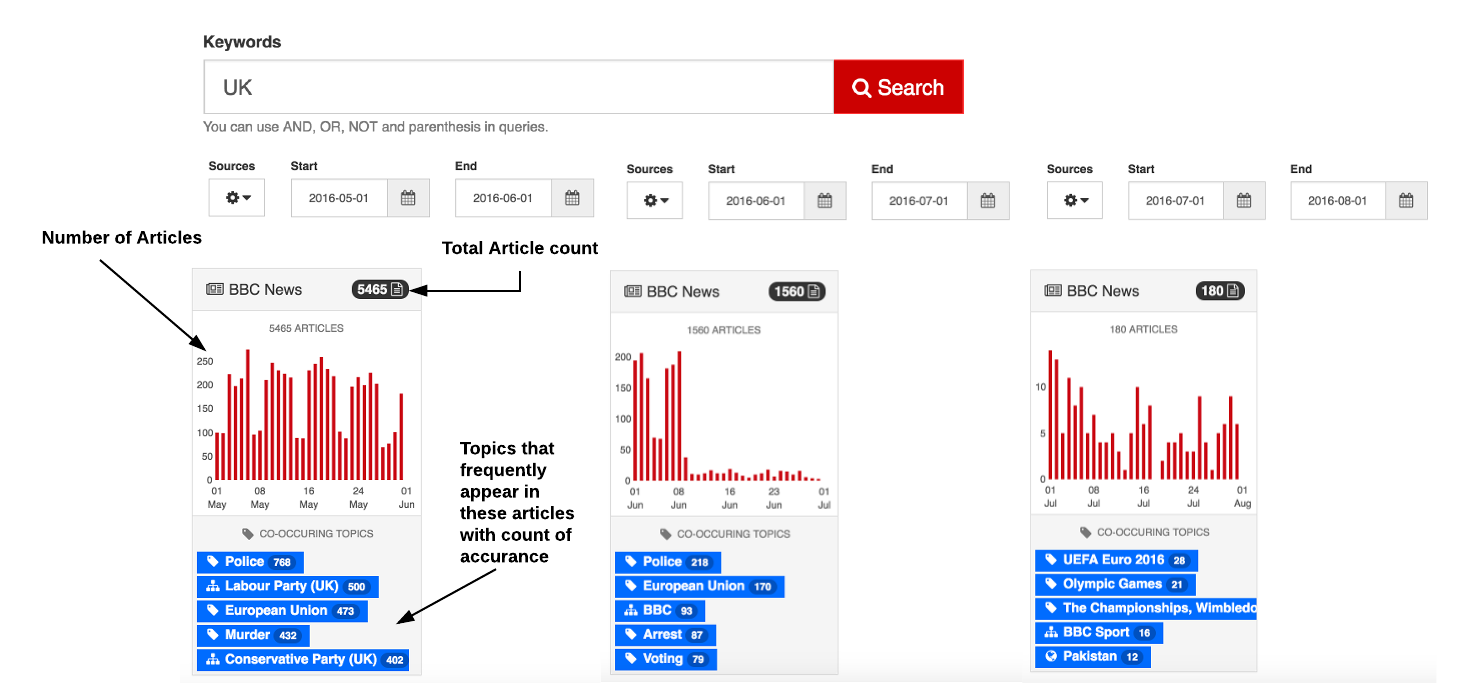
\includegraphics[width=\textwidth]{figures/BBC_wat.png}
\caption{Example of the topic evolution on BBC News: Who's talking about what ?}
\label{fig:bbc_wat}
\end{figure}

The other challenge is to apply Author-Topic (AT) model for the news collection which simultaneously model the content of the document and also the interest of the authors. The advantage of AT model is that besides representing each news with a mixture of topics, the \textit{author} is also modeled by determining the mixture weights for different topics for a single news, each \textit{author} is associated with a multinomial distribution over topics. This generative model perfectly fits in the corpus of BBC news, since for BBC news there is a virtual \textit{author} for each of the news, which is its category, as shown in ~\ref{tab:news_category}. For news in different categories their prose style will differ in the aspects of vocabulary use, sentence structure, as well as the way in which stories present the information in terms of relative importance, tone, and intended audience. 

Thus BBC news can be assumed to be generated in the following way, as shown in Figure~\ref{fig:author_diagram}.

\begin{enumerate}
   \item For each topic $k \in [1,K]$
   \begin{enumerate}
     \item Draw a multinomial $\vec{\phi_k}$ from a Dirichlet prior $\vec{\beta}$
    \end{enumerate}
   \item For each author $a \in [1,A]$
   \begin{enumerate}
     \item Draw a multinomial $\vec{\theta_a}$ from a Dirichlet prior $\vec{\alpha}$
    \end{enumerate}
    \item For each news $m \in [1,M]$
   \begin{enumerate}
     \item For each word $n \in [1,N_m]$ in document $m$
     \begin{enumerate}
            \item Draw an author $x_{m,n}$ uniformly from the group of authors $a_M$
            \item Draw a topic assignment $z_{m,n}$ from per-author multinomila distribution over topic $\vec{\theta}_{x_{m, n}}$ %$\vec{\theta_{x_{m,n}}}$
            \item Draw a word $w_{m,n}$ from multinomial $\vec{\phi}_{z_{m, n}}$
            %$\vec{\phi_{z_{m,n}}}$
    \end{enumerate}
    \end{enumerate}
        
\end{enumerate}

In the above process the posterior distribution of topics are dependent on the information form the authors as well as the text of the news. The parameterization of the AT model can be seen in Section ~\ref{Author-Topic model}

\begin{figure}[h]
\centering
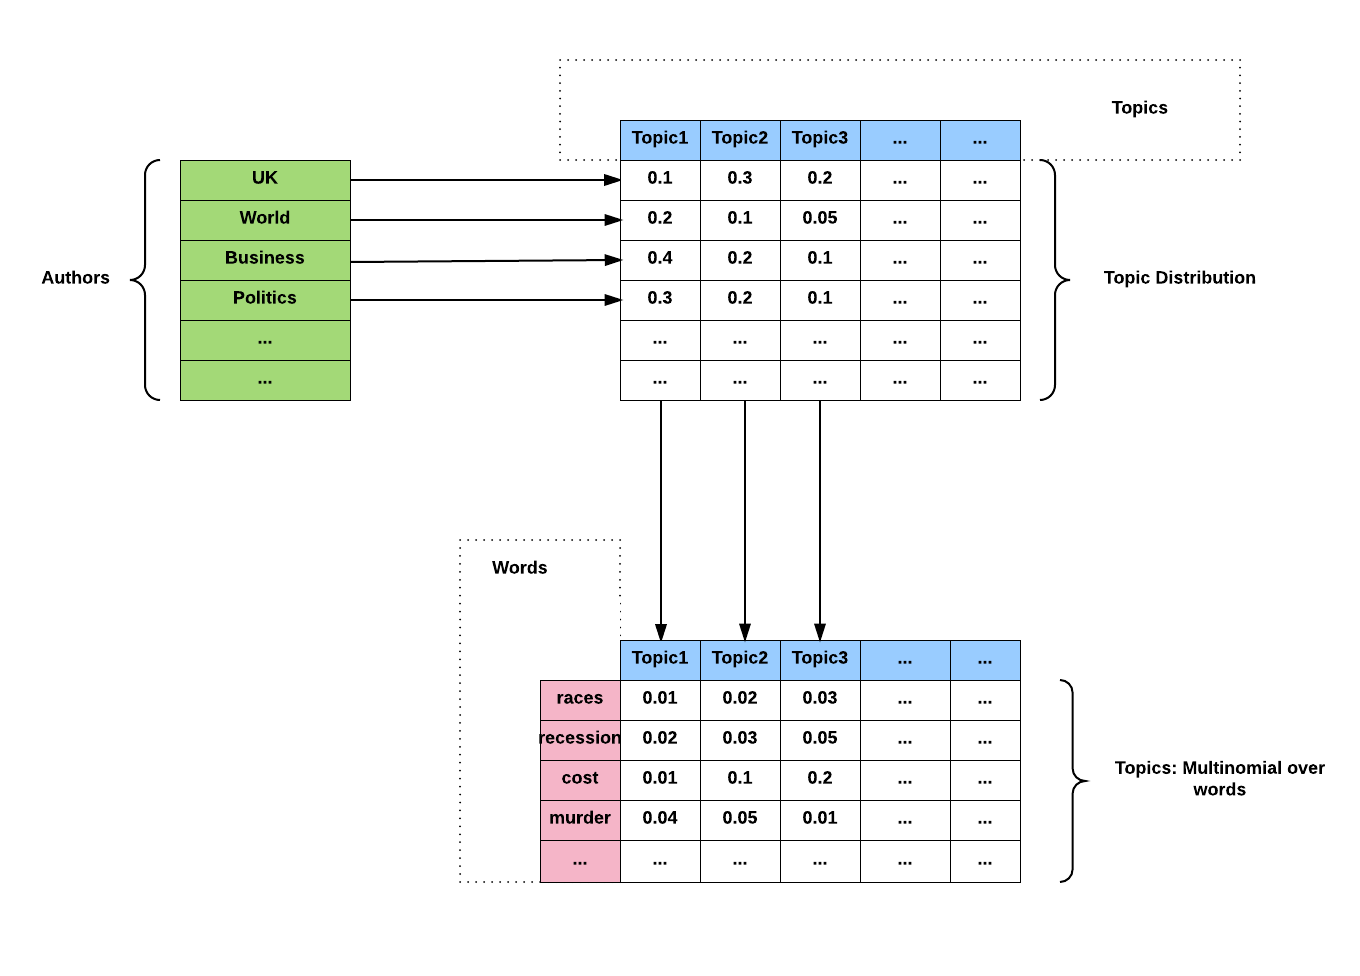
\includegraphics[width=\textwidth]{figures/author_diagram.png}
\caption{Illustration of Author Topic on BBC News Documents}
\label{fig:author_diagram}
\end{figure}


Therefore in order to encompass the extra-feature of the news, namely its category, in our model, the AT model is used as the basis of our dynamic model to overcome the above two challenges. Here we define the concepts of \textbf{\textit{topic}} and \textbf{\textit{author}} as follows,
\begin{itemize}
  \item A \textbf{\textit{topic}} is a subject discussed in one or more news. Examples of topics include events such as ``UK referendum" entities such as ``David Cameron" and long-standing subjects such as ``UK Politics". Each topic is assumed to be represented by acmultinomial distribution of words.
  \item An \textbf{\textit{author}} is a category of BBC news which groups topics belonging to a common subject
  area together. Examples of authors include BBC news categories of ``UK", ``World", ``Eduction", ``Health", etc, as listed in Table ~\ref{tab:news_category}
  \end{itemize}
The model we propose here is Dynamic Author-Topic (DAT) model which draws upon the strength of author-topic model and dynamic topic model. Considering the temporal nature of news we assume the topic distributions of news will evolve over time frames (a day, a week or a month), and the inferred topic distribution in the past news documents will become the evidence of those for the current new. In each time frame, we assume the news are generated based on author-topic model. Information about which topics are associated to which author and the representation of the content of each news document in terms of topics are derived and used for the next time frame. In Section ~\ref{taskdescription} we will discuss what kind of problem we want to solve using our proposed model. The details of the proposed model is further represented in Section ~\ref{dynamicauthortopicmodel}. Lastly we present how to infer the update rules for the hyperparameters as well as the multinomila parameters of our model using Collapsed Gibbs sampler in Section ~\ref{inferenceofthemodel}.

\section{Task Description}
\label{taskdescription}
The task to be addressed in this thesis can fall in the following three aspects:

\begin{itemize}
  \item \textbf{Tagging}: Based on the content and time of the news we are able to automatically tag the news with an author (category)
  \item \textbf{Summarization}: Based on the author-topic distribution we are able to what topics are most discussed in one type of news
  \item \textbf{Dynamics}: We are able to monitor the changes of event of interest for the news over time
\end{itemize}

The input data of our model will be the BBC news text in a range of time, as shown in Figure ~\ref{fig:input}.

\begin{figure}[h]
\centering
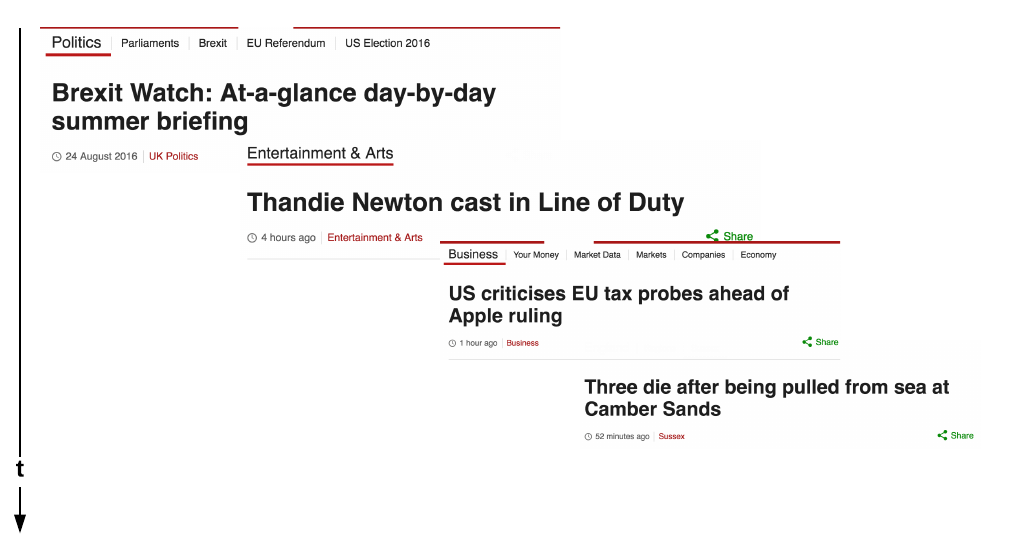
\includegraphics[width=\textwidth]{figures/input.png}
\caption{Input data: BBC News over time}
\label{fig:input}
\end{figure}
The output result will satisfy the above three aspects, as shown in Figure ~\ref{fig:output}.
\begin{figure}[h]
\centering
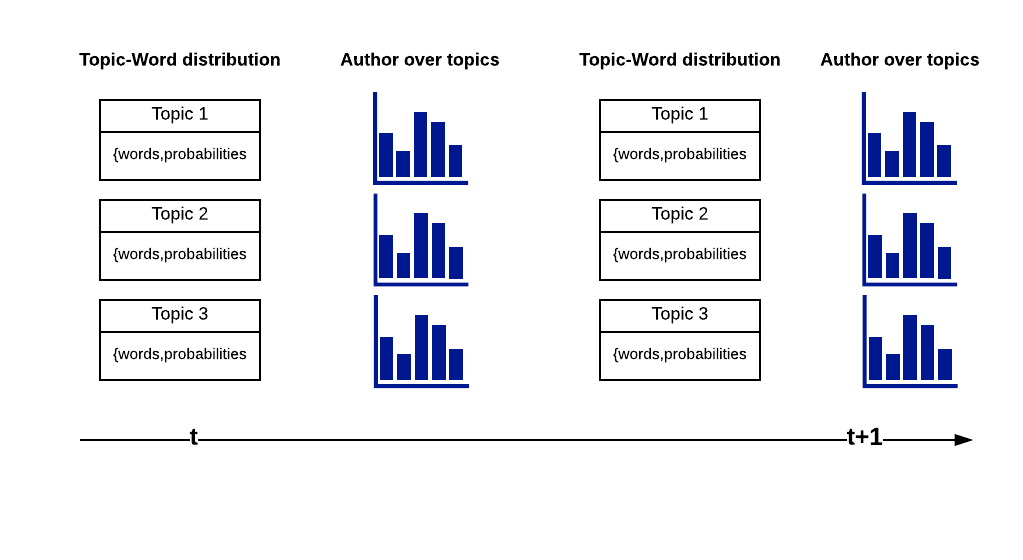
\includegraphics[width=\textwidth]{figures/output.png}
\caption{Output result: Temporal evolution of topics and authors’ proportion over the topics }
\label{fig:output}
\end{figure}



Mathematically, the author-topic and topic-words distribution are changing dynamically with news stream in, our dynamic model is essentially a function $f$ that satisfies:
\begin{equation}
\label{eq:task}
\mathbf{m}_{\le t}=\{\ldots, \mathbf{m}_{t-2}', \mathbf{m}_{t-1}', \mathbf{m}_t'\}
\stackrel{f}{\longrightarrow} \boldsymbol W'_{\boldsymbol a,\boldsymbol k}_{\le t}=\{\{\mathbf{w}_1', \mathbf{w}_2', \ldots, \mathbf{w}_K'\},\{\mathbf{w}_1', \mathbf{w}_2', \ldots, \mathbf{w}_A'\}\},
\end{equation}
where $\mathbf{m}_{\le t}$ represents news stream with $\mathbf{m}_t'$ being the most recent \textit{set} news, arriving at time $t$, with our dynamic model it results in  $\boldsymbol W'_{\boldsymbol a,\boldsymbol k}$ is the resulting set of 3-tuple, $\{w,a,k\}$, which represents word $w$ and the author $a$ and topic $k$ assigned to it, with $\mathbf{w}_k'$ being the words set associated with topic $k$,  with $\mathbf{w}_a'$ being the words set associated with author $a$-th. $\mathbf{m}'_t$ comprises a the stream of news at time $t$, with each news $m$ being represented by a sequence of words appearing in $m$, coming from the vocabulary $\boldsymbol w$. % and $t$ is the creation time of the document $d$.
%$\mathbf{d}'_t$ comprises a set of short text documents, with each document being represented by a tuple $\langle \mathbf{w}_d, t \rangle$ where $\mathbf{w}_d$ is a sequence of words appearing in document $d$, coming from a vocabulary $\mathbf{V}=\{ v_1, v_2, \ldots, v_V\}$, and $t$ is the creation time of the document $d$. 

Based on $\boldsymbol W'_{\boldsymbol a,\boldsymbol k}$ we are able to calculate the author-topic and topic-word distribution to see the topic evolution over time.
Table ~\ref{tab:notation-des} summarises the main notations that we have used in our dynamic author-topic model.
\begin{table}[h]
\center
\vspace{-1pt}
\caption{Notation used in the Dynamic Author-topic model}
\label{tab:notation-des}
\small
\begin{tabular}{ll}
%\toprule
Symbol & Description\\
\hline

$\bs{K}$ & Number of latent topics\\
$\bs{M}$ & Number of news\\
$\bs{A}$ & Number of unique authors\\
$\bs{A_m}$ & Number of authors in document $m$\\
$\bs{V}$ & Number of unique word tokens in the whole news corpus\\
$T$ & Number of time frames  \\
$N_{\text{m}}$ & Number of word tokens in news m\\
$k$ & Topic index,  $k \in [1,\bs{K]$ \\
$m$ & News index,  $m \in [1,M]$ \\
$a$ & Author index,  $a \in [1,\bs{A}]$ \\
$t$ & Time frame index, $t \in [1,T]$\\
$n$ & Word index in document $m$,  $n \in [1,N_{\text{m}}]$ \\
$v$ & Word index in the whole news document corpus,  $v \in [1,V]$ \\
$\boldsymbol a$ & Set of all authors \\
$\boldsymbol k$ & Set of all topics \\
$\boldsymbol m$ & Set of all news \\
$\boldsymbol m'_t$ & Set of news at time t\\
$\boldsymbol w$ & Words set for all news \\
$\boldsymbol w'_{a}$ & Words set comprising words associated with author $a$ \\
$\boldsymbol w'_{k}$ & Words set comprising words associated with topic $k$ \\
$\boldsymbol W'_{\boldsymbol a,\boldsymbol k}$ & The set of 3-tuple, $\{w,a,k\}$, which represents word $w$ and the author $a$ \\
& and topic $k$ assigned to it \\
$\boldsymbol w_m$ & Words set for news $m$ \\
$\alpha_{t}$ & Parameter of topic Dirichlet prior to $\theta$ at time $t$ \\
$\beta{t}$ & Parameter of word Dirichlet prior to $\phi$ at time $t$ \\
$a_m$ & Authors in news m,  $a_m \in [1,\bs{A]$ \\
$\theta_{a,t}$ & Dynamic multinomial distribution of topics specified to author $a$ at time $t$ \\
$\phi_{k,t}$ & Dynamic multinomial distribution of words specified to topic $k$ at time $t$ \\
$x_{m,n}$ & Author associated to $w_{m,n}$ \\
$z_{m,n}$ & Topic associated to $w_{m,n}$ \\
$w_{m,n}$ & $n_{th}$ word in doc $n$ \\
%\bottomrule

\hline
\end{tabular}
\end{table}

\section{Dynamic Author-Topic Model}\label{dynamicauthortopicmodel}
To meet the requirements discussed in ~\ref{taskdescription}, so that the event interests of the news can be sequentially inferred using the newly published news. For the news its hot topics and trends change over time but writing styles of the news of the same category will keep stable. So that we propose the Dynamic Author-Topic (DAT) model here which is adaptable to changes and also is an incremental model in which updates can be achieved. Our model is able to reflect the news' reality of rapid change and has the capability to deal with accumulated huge amount of data in the real online system.
\subsection{Preliminaries}
The target of the DAT model is to infer the dynamically changing topic-word distribution and author-topic distribution at any given time $t$ with continuously incoming news stream. Therefore, we need to infer the temporal word, $v$'s probability for a topic $z$, $P(v|t, z)$, and the temporal topic probability over an author $a$, which in our case is the news' category, $P(z|t, a)$. Then we can obtain,
\begin{equation}
p(v|t,a) = \sum_{z=1}^Z{P(v|t, z)P(z|t, a)},
\end{equation}
which represents the association between the word $v$ and the author $a$, which can be used to automatically classify the news into BBC news category.
\def \thetadef {$\boldsymbol{\Theta}_{a,t}=\{\theta_{a,t, z}\}_{z=1}^Z$}
\def \phidef {$\boldsymbol{\Phi}_t=\{\phi_{t, z}\}_{z=1}^Z$}

Based on the probabilistic model, \thetadef is the topic distribution associated with author $a$, at time $t$ with  $\sum_{a=1}^A\sum_{z=1}^Z\theta_{a, t, z}=1$. We also let \phidef be the words distribution over topics at time $t$. $\phi_{t, z}=\{\phi_{t, z, v}\}_{v=1}^V$ is the multinomial distribution of the words for topic $z$ at time $t$, and also the probability of a word $v$ belonging to $z$ at $t$, $\phi_{t, z, v}=P(v|t, z)>0$, and $\sum_{v=1}^V \phi_{t, z, v}=1$. There is an underlying assumption of the fully bayesian non-dynamic topic models that the topic distribution over an author is independent of the past trends of the news, with a Dirichlet prior with a static set of parameters $\kappa=\{\kappa_z\}_{z=1}^Z$, with $\kappa_{z}>0$,
\begin{equation}
\label{eq:assume1}
P(\boldsymbol{\Theta}_{a,t} | \kappa)  \propto \prod_{z=1}^Z \theta_{a, t, z}^{\kappa_z -1},
\end{equation}
Since the news is actually a continuous stream data, therefore the assumptions made in~\eqref{eq:assume1} is not always realistic. So two assumptions are be made for our temporal dependent model. Firstly the means of the author-topic distribution at the moment are the same as those at a previous time point unless otherwise confirmed by the newly coming-in data. Secondly, we assume that in a short time-period the trends and topics of the news remain static, which means that the author-topic distribution at time $t$ will remain the same as that at time $t-1$ if no news is observed, and it will be updated when new set of documents come in at time $t+1$. Hence, the Dirichlet parameter in \eqref{eq:assume1} can be factorized into the mean of the distribution at the previous time-step, $\theta_{a,t-1,z}$ and a set of prevision value, $a = \{a_{t,z}\}_{z=1}^Z$, representing the topic persistency on topic $a$. Hence, $\kappa=\alpha_t \boldsymbol{\Theta}_{a,t-1}$, which allows the mean of the current distribution $\boldsymbol{\Theta}_{a,t}$ to depend on the mean of the previous distribution $\boldsymbol{\Theta}_{a,t-1}$.

\begin{equation}
\label{eq:shortTheta}
P(\boldsymbol{\Theta}_{a,t} | \boldsymbol{\Theta}_{a,t-1}, \alpha_t) \propto \prod_{z=1}^Z \theta_{a,t, z}^{(\alpha_{t, z} \theta_{a,t-1, z}) -1},
\end{equation}
And similarly, the word distribution over per topic, $\phi_{t, z}$ also has a Dirichlet prior with a static set of parameters $\gamma=\{\gamma_v\}_{v=1}^V$, with $\gamma_v>0$, 
\begin{equation}
\label{eq:assume2}
P(\boldsymbol{\phi}_{t, z} | \gamma) \propto \prod_{v=1}^V \phi_{t, z, v}^{\gamma_v -1},
\end{equation}
the Dirichlet prior parameter $\gamma$ in above can be also factorized into the mean and precision, $\gamma=\beta_{t, z} \phi_{t-1, z}$,  $\beta_t=\{\beta_{t, z}\}_{z=1}^Z$ are the set of precision values at time $t$ for the topics. Here $\beta_{t, z, v}$ represents the persistency of word $v$ in topic $z$ at time $t$, used to measure how consistently word $v$ belongs to topic $z$ at time $t$ compared to that at the previous time $t-1$. Therefore, we can obtain another dependency distribution formula:

\begin{equation}
\label{eq:shortPhi}
P(\phi_{t, z} | \phi_{t-1, z}, \beta_{t, z}) \propto \prod_{v=1}^V \phi_{t, z, v}^{(\beta_{t, z, v} \phi_{t-1, z, v}) -1}.
\end{equation}
The distributions in ~\eqref{eq:shortTheta} and ~\eqref{eq:shortPhi} are conjugate priors of the Multinomial distribution, thus the inference can be performed by Gibbs sampling~\cite{liu1994collapsed} with details showing in Section ~\ref{inferenceofthemodel}.
%
\subsection{Description of the Model}


In Section \ref{taskdescription} we have presented how we model our dynamic author-topic model by considering the temporal factor. In this section we will further describe our model in detail. 

\begin{figure}[h]
\centering
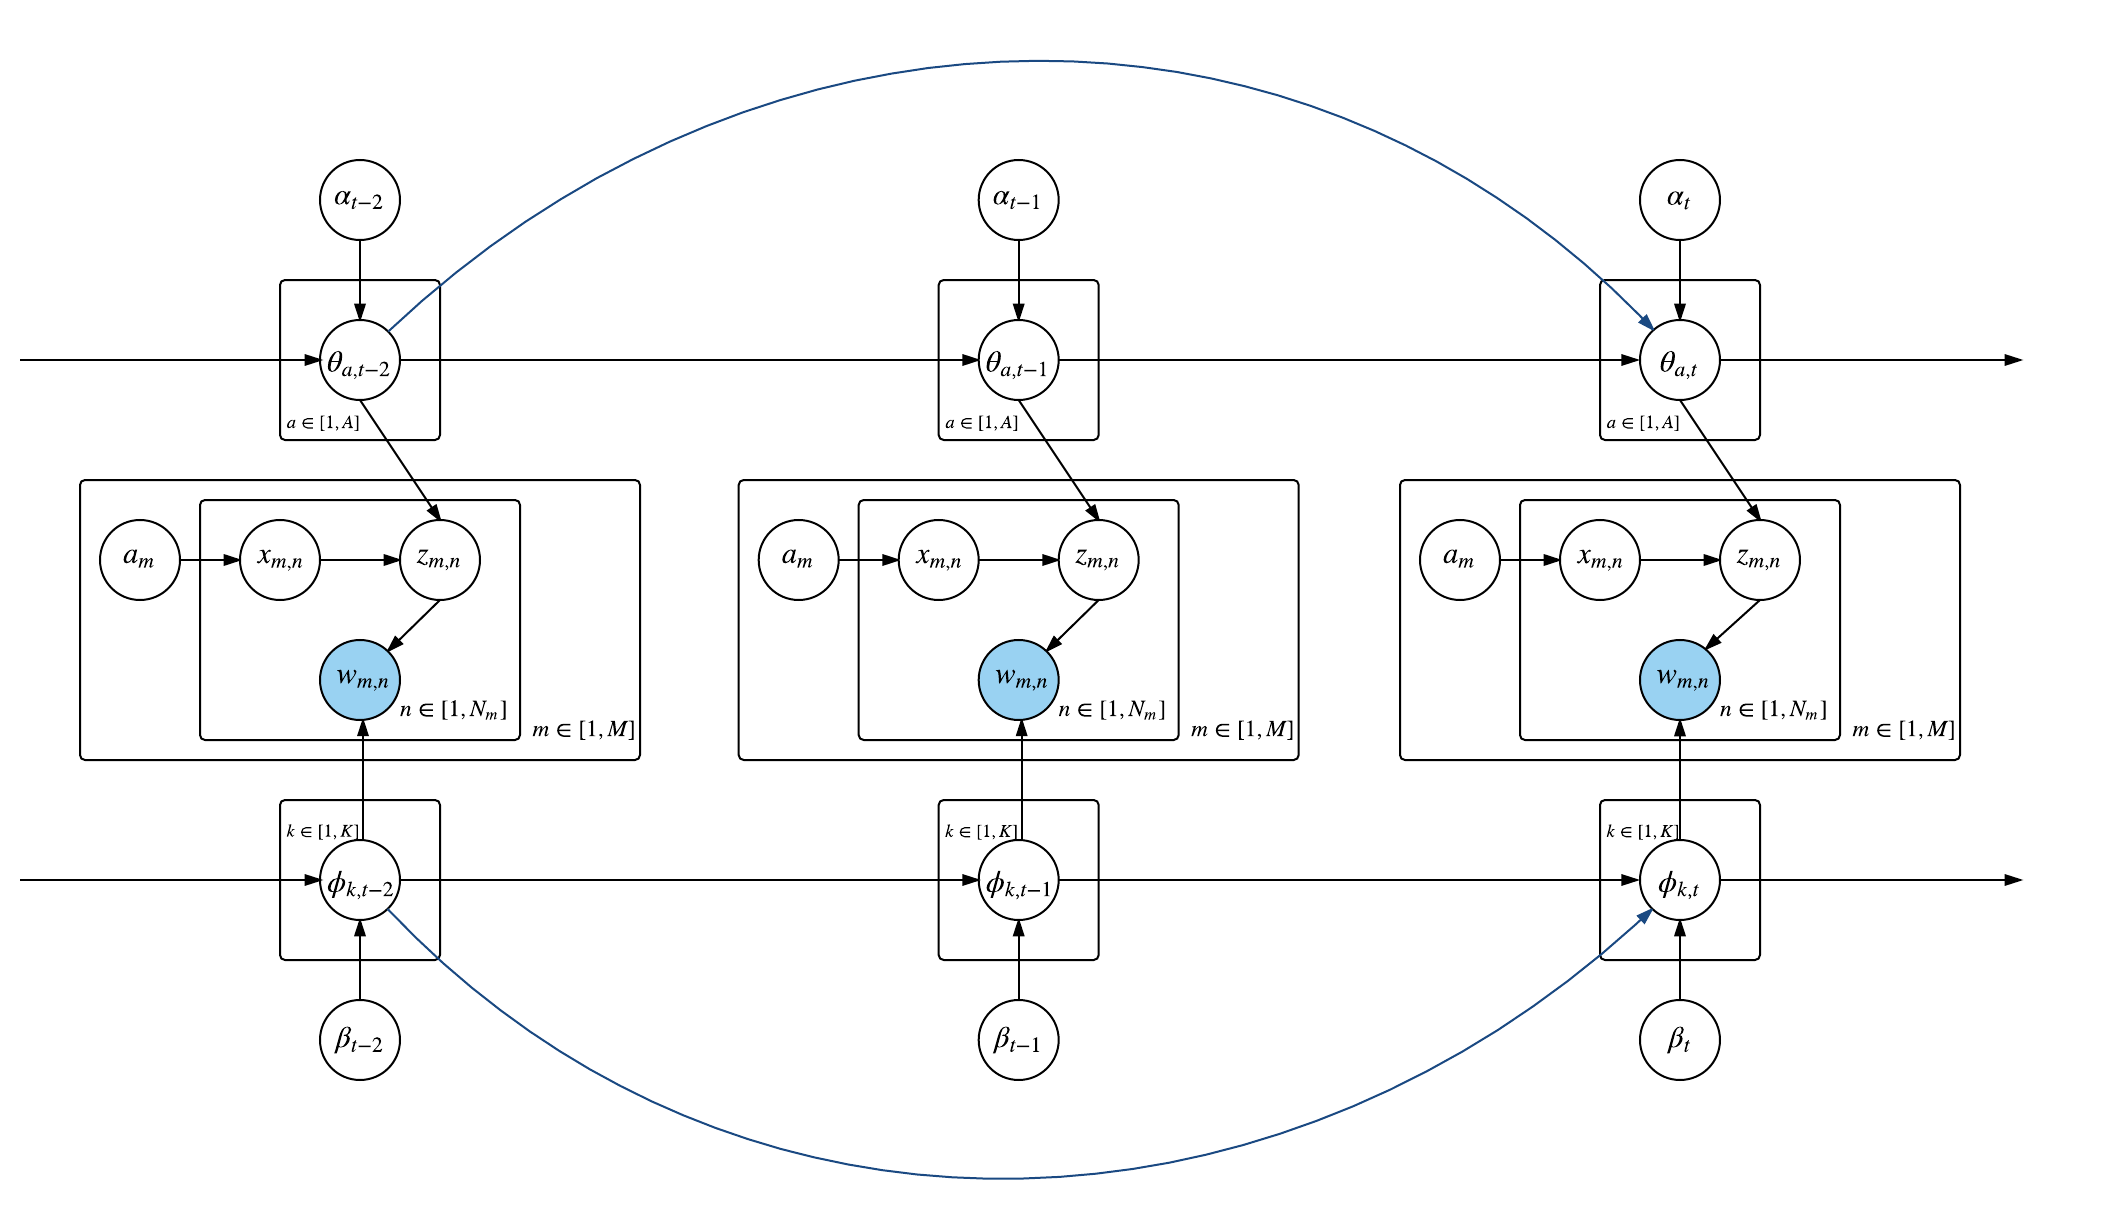
\includegraphics[width=1.1\textwidth]{figures/ATOT_Graphic.png}
\caption{Graphical representation of our dynamic author-topic model, DAT model. Note that short term dependency DAT model excludes the two blue curved lines , whereas the long term dependency DAT model includes the two lines.}
\label{fig:atot}
\end{figure}


Figure~\ref{fig:atot} illustrates the graphical representation of the Dynamic Author-Topic model, on conditional that we have computed the topic distribution over authors at time $t-1$, $\boldsymbol{\Theta}_{a,t-1}$, and the word distribution over topics at time $t-1$, $\boldsymbol{\Phi}_{t-1}$, as well as the hyperparameters $\alpha_{t-1}$ and  $\beta_{t-1}$. The parameterization of our proposed model for news stream  at time $t$, is as follows,

\begin{eqnarray*} \label{eq:dat}
\boldsymbol{\Theta}_{a,t} | \boldsymbol{\alpha_{a,t}}
\boldsymbol{\Theta}_{a,t-1}
& \sim & \text{Dirichlet}({\boldsymbol{\alpha_{a,t}}
\boldsymbol{\Theta}_{a,t-1}})\\
\boldsymbol{\Phi_{k,t}} | \boldsymbol{\beta_{k,t}}\boldsymbol{\Phi_{k,t-1}} & \sim & \text{Dirichlet}(\boldsymbol{\beta_{k,t}}\boldsymbol{\Phi_{k,t-1}})\\
z_{m,n} | \boldsymbol{\Theta_{x_{m,n},t}} & \sim & \text{Multinomial}(\boldsymbol{\Theta_{x_{m,n},t}})\\
w_{m,n} | \boldsymbol{\Phi_{z_{m,n},t}} & \sim & \text{Multinomial}(\boldsymbol{\Phi_{z_{m,n},t}})\\
x_{m,n} | {A_{m}} & \sim & \text{Multinomial}(1/A_m)\\

\end{eqnarray*}

As in author-topic model each topic $z$ is sampled from an author-specific multinomial distribution and each word $w$ is sampled from a topic-specific multinomila distribution.

the generative process of our model on the news stream at time $t$ is as follows,
\begin{enumerate}
   \item For each topic $k \in [1,K]$
   \begin{enumerate}
     \item Draw a multinomial $\vec{\phi_{t,k}}$ from a Dirichlet prior $\vec{\beta_{t,k}}\vec{\phi_{t-1,k}}$
    \end{enumerate}
   \item For each author $a \in [1,A]$
   \begin{enumerate}
     \item Draw a multinomial $\vec{\theta_{a,t}}$ from a Dirichlet prior $\vec{\alpha_{a,t}}\vec{\theta{t-1,a}}$
    \end{enumerate}
    \item For each news $m \in [1,M]$
   \begin{enumerate}
     \item For each word $n \in [1,N_m]$ in document $m$
     \begin{enumerate}
            \item Draw an author $x_{m,n}$ uniformly from the group of authors $a_M$
            \item Draw a topic assignment $z_{m,n}$ from per-author multinomila distribution over topic $\vec{\theta}_{x_{m, n},t}$ %$\vec{\theta_{x_{m,n},t}}$
            \item Draw a word $w_{m,n}$ from multinomial $\vec{\phi}_{z_{m, n},t}$
            %$\vec{\phi_{z_{m,n},t}}$
    \end{enumerate}
    \end{enumerate}
        
\end{enumerate}


Since the inference of the distribution of our proposed model is intractable, therefor Gibbs sampler as discussed in \cite{wang2006topics} is used for parameter estimation, we adopt a Dirichlet prior for the multinomila distribution which is its conjugate, thus the uncertainty associated with $\boldsymbol{\Phi_t}$ and $\boldsymbol{\Theta_t}$ can be easily integrated out. In the Gibbs sampling procedure our target is to calculate the conditional distribution at time $t$, which is
$P({z}_{m, n, t},{x}_{m, n, t}| \mathbf{w}_t,\mathbf{z}_{\neg(m, n, t)}, \mathbf{x}_{\neg(m, n, t)},\mathbf{a_t},\alpha_t, \beta_t,\boldsymbol{\Phi}_{t-1}, \boldsymbol{\Theta}_{t-1})$.
The process of model inference is discussed in Section ~\ref{inferenceofthemodel}. Briefly, using the chain rule we can finally obtain the following joint probability in \ref{joint} , 

\begin{align}\label{joint}
\multicolumn{2} =   &  \math{P}({z}_{m, n, t},{x}_{m, n, t}| \mathbf{w}_t,\mathbf{z}_{\neg(m, n, t)}, \mathbf{x}_{\neg(m, n, t)},\mathbf{a_t},\alpha_t, \beta_t,\boldsymbol{\Phi}_{t-1}, \boldsymbol{\Theta}_{t-1}) \nonumber
\displaybreak[3]\\  \nonumber
\propto & \quad  \left(\frac{n_{t,v,k}+\beta_{t,k,v}\phi_{t-1}-1}{\sum_{v=1}^V \left(n_{t,v,k}+\beta_{t,v,k}\phi_{t-1} \right)-1 } \right) \times   \left(\frac{n_{t,a,k}+\alpha_{t,k} \Theta_{t-1}-1}{\sum_{k=1}^K \left(n_{t,a,k}+\alpha_{t,k}\theta_{t-1} \right)-1 } \right)
\displaybreak[3]\\
\end{align}
 
The joint probability in \ref{joint} can be then turned  into the separated update rules for associated topic and author of a work token. The update rule for topic is shown in \ref{topic_update_rule} and the one for the author is \ref{author_update_rule}.


\begin{align}\label{topic_update_rule}
\multicolumn{2} =   &  \math{P}({z}_{m, n, t}| \mathbf{w}_t,\mathbf{z}_{\neg(m, n, t)},\mathbf{x}_t, \mathbf{a_t},\alpha_t, \beta_t,\boldsymbol{\Phi}_{t-1}, \boldsymbol{\Theta}_{t-1}) \nonumber
\displaybreak[3]\\ \nonumber
\propto & \quad  \left(\frac{n_{t,v,k}+\beta_{t,k,v}\phi_{t-1}-1}{\sum_{v=1}^V \left(n_{t,v,k}+\beta_{t,v,k}\phi_{t-1} \right)-1 } \right) \times   \left(\frac{n_{t,a,k}+\alpha_{t,k} \Theta_{t-1}-1}{\sum_{k=1}^K \left(n_{t,a,k}+\alpha_{t,k}\theta_{t-1} \right)-1 } \right)
\displaybreak[3]\\
\end{align}
  
\begin{equation}\label{author_update_rule}
 \math{P}({x}_{m, n, t}| \mathbf{z}_t,\mathbf{x}_{\neg(m, n, t)}, \mathbf{a_t},\alpha_t,  \boldsymbol{\Theta}_{t-1}) \quad
\propto  \quad   \left(\frac{n_{t,a,k}+\alpha_{t,k} \Theta_{t-1}-1}{\sum_{k=1}^K \left(n_{t,a,k}+\alpha_{t,k}\theta_{t-1} \right)-1 } \right)
\displaybreak[3]\\
\end{equation}

 \eqref{topic_update_rule} and \eqref{author_update_rule} are used to update $x_{m,n}$ and $z_{m,n}$ for each iteration, by maximizing the joint distribution \ref{joint} the precision parameters can be estimated, the fixed point iteration is applied to get the optimal $\alpha$ and $\beta$ at time $t$ and the following update rules are obtained with details in Section ~\ref{inferenceofthemodel}. 
 \begin{equation}\label{dat_alpha1}
 \quad \alpha^*_{t,k} \gets \frac{\sum_{a=1}^A \alpha_{t, k}(\psi(n_{a,t,k}+\alpha_{t, k} \theta_{t-1, k})-\psi(\alpha_{t,k}\theta_{t-1, k}))}{\sum_{a=1}^A (\psi(\sum_{k=1}^K(\alpha_{t, k} \theta_{t-1, k}+n_{t,a,k}))-\psi(\sum_{k=1}^K(\alpha_{t, k} \theta_{t-1, k})))}  \displaybreak[3]\\
\end{equation}

\begin{equation}\label{eq:beta1}
 \beta^*_{t,k,v} \gets \frac{\sum_{k=1}^K \beta_{t,v,k}\phi_{t-1}(\psi(\beta_{t,k,v}\phi_{t-1}+n_{t,v,k})-\psi(\beta_{t,v,k}\phi_{t-1}))}
{   \sum_{k=1}^K(\psi(\sum_{v=1}^V(\beta_{t,k,v}\phi_{t-1}+n_{t,v,k})) -\psi(\sum_{v=1}^V\beta_{t,k,v}\phi_{t-1}))\phi_{t-1}}     
\end{equation}

By iterating Gibbs sampling with ~\ref{topic_update_rule} and ~\ref{author_update_rule} and maximum likelihood estimation with ~\ref{dat_alpha1} and ~\eqref{eq:beta1}, we can estimate the latent topics $\vec{z}$, authors $\vec{a}$, and parameters $\alpha$ and $\beta$ for each time point.

After the iteration the means of $\phi_{k,v,t}$ and $\theta_{a,k,t}$ can be obtained based on \ref{dat_phi1} and \ref{dat_theta1}, these estimation are used to estimate the news trend for the next time period $t+1$.

\begin{equation}\label{dat_phi1}
\phi_{k,v,t} = \left(\frac{n_{t,v,k}+\beta_{t,k,v}\phi_{t-1}}{\sum_{v=1}^V \left(n_{t,v,k}+\beta_{t,v,k}\phi_{t-1} \right) } \right) 
\end{equation}
\begin{equation}\label{dat_theta1}
\theta_{a,k,t} = \left(\frac{n_{t,a,k}+\alpha_{t,k} \Theta_{t-1}}{\sum_{k=1}^K \left(n_{t,a,k}+\alpha_{t,k}\theta_{t-1} \right) } \right)
\end{equation}


From the perspective of engineering system, we only use the current data when inferring the current author-topic and topic-word distribution $\boldsymbol{\Theta_{a,k}}$ and $\boldsymbol{\Phi_{w,k}}$, the computational and storage complexity can be largely reduced compared to traditional model which are relied on past data. The processing flow of our DAT model is shown in Figure ~\ref{fig:flow}. 


\begin{figure}[h]
\centering
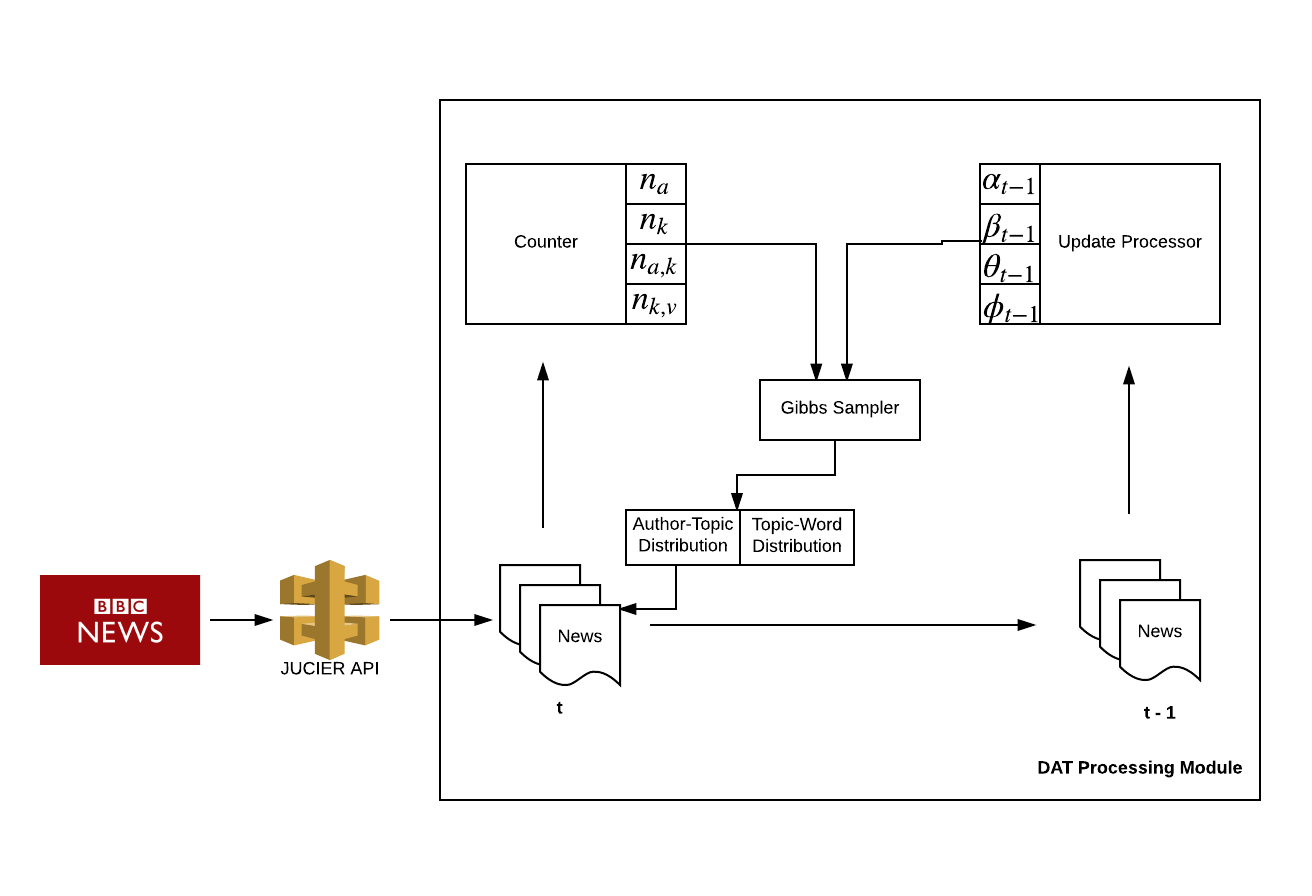
\includegraphics[width=1.1\textwidth]{figures/model_description.png}
\caption{Flow Diagram of Dynamic Author-Topic model: An Example between time $t-1$ and $t$}
\label{fig:flow}
\end{figure}

So for each time period only the parameters that are needed by the inference for the next period will be remaining with unnecessary data removed. Therefore our model outperforms conventional LDA and Author-topic model in terms of time and memory efficiency.

The Gibbs Sampler can be realized with the procedure in Algorithm 1, the Gibbs sampling algorithm runs over the three periods of initialization, burn-in and sampling. We assume that our document corpus is a stream of news spanning time period $T$, our Gibbs sampler is ran for each time point $t$ where $t \in [1,T]$. Before the first set of news come into our processing module, namely at time $t = 0$, no previous information is available so all parameters are initialized at this time. After that, our author-topic and topic-word distribution as well as the precision values will be updated based on those of last time. Here $M_t$ represents the total number of news at time period $t$, while $N_{m,t}$ is the total number of unique words from $M_t$ number of news.

\begin{algorithm}\label{algo:ATOT}
\DontPrintSemicolon
\LinesNumbered
 
    \SetKwInOut{Input}{Input}
    \SetKwInOut{Output}{Output}
    \SetKwInOut{Parameter}{Global Data}

    \Input{word vector $\boldsymbol{w}$, author vector $\boldsymbol{a}$, $\alpha$,$\beta$, topic number $K$}
    \Parameter{count statistics $\{n_{a,k}\}$, $\{n_{k,v}\}$, and their sums $\{n_{a}\}$, $\{n_{k}\}$}
    \Output{topic associations $\boldsymbol{z}$, author associations $\boldsymbol{a}$, multinomila parameter $\boldsymbol{\Phi}$, and $\boldsymbol{\Theta}$}
    \If{$t=0$}{
    Set initial values for $\boldsymbol{\Theta}$ as $1/K$ and $\boldsymbol{\Phi}$ as $1/V$, also for $\boldsymbol{\alpha}$ and $\boldsymbol{\beta}$  
    }
    \For{time $t \in [1,T]$}{
    {//  
    \textbf{Initialization}:}\;
    zero all count variables: $\{n_{a,k}\}$, $\{n_{k,v}\}$, $\{n_{a}\}$, $\{n_{k}\}$\, 
    \For{all news $m \in [1,M_t]$ }{
      \For{all words $n \in [1,N_{m,t}]$ in news m }{
      sample topic index $z_{m,n} = k \sim \text{Multinomial}(1/K)$ \par
      sample author index $x_{m,n} = a \sim \text{Multinomial}(1/A_m)$ \par
      increment author-topic count: $n_{a,k} += 1$\par
      increment author-topic sum: $n_{a} += 1$\par
      increment topic-word count: $n_{k,w_{m,n}} += 1$\par
      increment topic-word count: $n_{k} += 1$\par
      }
   }
   
  
   {// \textbf{Gibbs Sampling}:}\;
    sample over burn-in period and sampling period:\; 
    \caption{Inference for the Dynamic Author-Topic model model using Gibbs sampling }
    \While{not finished}{
    \For{all news $m \in [1,M_t]$ }{
      \For{all words $n \in [1,N_{m,t}]$ in news m }{
      // For the current assignment of $k$ and $a$ to the word token $w_{m,n}$ \par
      decrement author-topic count: $n_{a,k} -= 1$\par
      decrement author-topic sum: $n_{a} -= 1$\par
      decrement topic-word count: $n_{k,w_{m,n}} -= 1$\par
      decrement topic-word count: $n_{k} -= 1$\par
      sample author index $\boldsymbol{a} \sim \math{P}({x}_{m, n, t}| \mathbf{z}_t,\mathbf{x}_{\neg(m, n, t)}, \mathbf{a_t},\alpha_t,  \boldsymbol{\Theta}_{t-1}) $ according to Eq. \ref{author_update_rule} \par
      sample topic index $\boldsymbol{z} \sim \math{P}({z}_{m, n, t}| \mathbf{w}_t,\mathbf{z}_{\neg(m, n, t)},\mathbf{x}_t, \mathbf{a_t},\alpha_t, \beta_t,\boldsymbol{\Phi}_{t-1}, \boldsymbol{\Theta}_{t-1})$ according to Eq. \ref{topic_update_rule}\par
      // For the new assignment of $k$ and $a$ to the word token $w_{m,n}$ \par
      increment author-topic count: $n_{a,k} += 1$\par
      increment author-topic sum: $n_{a} += 1$\par
      increment topic-word count: $n_{k,w_{m,n}} += 1$\par
      increment topic-word count: $n_{k} += 1$\par
      
      }
   }
   Update prevision value $\boldsymbol{\alpha_t}$ according to Eq. \ref{dat_alpha1}\par
    Update prevision value $\boldsymbol{\beta_t}$ according to Eq. \eqref{eq:beta1}\par
    }
    \If{converged}{
    Update parameter set $\boldsymbol{\Phi_t}$ according to Eq. \ref{dat_phi1}\par
    Update parameter set $\boldsymbol{\Theta_t}$ according to Eq. \ref{dat_theta1}\par
    
    $t= t + 1$
    }
    }
\end{algorithm}







\section{Inference}\label{inferenceofthemodel}

Similar to LDA model, based on the algorithm proposed by \cite{blei2003latent} to calculate the approximate maximum likelihood estimates for $\boldsymbol{\phi}$ as well as the hyperparameter of the prior $\boldsymbol{\theta}$, the Markov Chain Monte Carlo (MCMC) is used for inference, MCMC is an approach to obtain the sample from the complicated probability distributions, to allow a Markov chain to converge to a targeted distribution and the drawing the samples from the Markov chain \cite{gilks1996introducing}. Since the inference of the parameters of the distribution of the model is intractable, so collapsed Gibbs Sampling is used here for the inference in which the next state is arrived by sampling all variables from their distribution sequentially when conditioned on the current values of all other variables and the data.
in the above Gibbs sampling procedure, we need to calculate the conditional distribution first, which is
\begin{equation}
P({z}_{m, n, t},{x}_{m, n, t}| \mathbf{w}_t,\mathbf{z}_{\neg(m, n, t)}, \mathbf{x}_{\neg(m, n, t)},\mathbf{a_t},\alpha_t, \beta_t,\boldsymbol{\Phi}_{t-1}, \boldsymbol{\Theta}_{t-1})
\label{eq:conditional}
\end{equation}
where $\mathbf{z}_{\neg(m, n, t)}, \mathbf{x}_{\neg(m, n, t)}$ represents the topic, author assignments for all the word tokens in the news corpus except for $w_{m,n}$. We can begin with the joint distribution,
\begin{equation}
P(\mathbf{w}_t, \mathbf{z}_t ,\mathbf{x}_t| \alpha_t, \beta_t,\mathbf{a}, \boldsymbol{\Phi}_{t-1}, \boldsymbol{\Theta}_{t-1})
\end{equation}
so that we can take advantage of the conjugate priors to simplify the integrals. The symbols used here are all defined in Table~\ref{tab:notation-des}. The whole process of Gibbs sampling derivation for our dynamic author-topic model is listed as follows.
\begin{align*}
\multicolumn{2} =   &  \math{P}({z}_{m, n, t},{x}_{m, n, t}| \mathbf{w}_t,\mathbf{z}_{\neg(m, n, t)}, \mathbf{x}_{\neg(m, n, t)},\mathbf{a_t},\alpha_t, \beta_t,\boldsymbol{\Phi}_{t-1}, \boldsymbol{\Theta}_{t-1})
\displaybreak[3]\\
\propto & \quad P(\mathbf{w}_t, \mathbf{z}_t ,\mathbf{x}_t| \alpha_t, \beta_t,\mathbf{a_t}, \boldsymbol{\Phi}_{t-1}, \boldsymbol{\Theta}_{t-1}) \displaybreak[3]\\
& \hspace{-0.1in}\text{based on the graphical model in Figure ~\ref{fig:atot}, and integrate on $\boldsymbol{\Phi}$ and $\boldsymbol{\Theta}$ it becomes}\displaybreak[3]\\
= & \quad  P(\mathbf{w}_t | \mathbf{z}_t, \mathbf{\beta}_t,\boldsymbol{\Phi}_{t-1})\times P(\mathbf{z}_t | \boldsymbol{\Theta}_{t-1}, \alpha_t, \mathbf{x}_t) \times P(\mathbf{x}_t | \mathbf{a}_t) \displaybreak[3]\\
= & \quad \int P(\mathbf{w}_t | \mathbf{z}_t, \boldsymbol{\Phi}_t) P(\boldsymbol{\Phi}_t | \boldsymbol{\Phi}_{t-1}, \beta_t) d\boldsymbol{\Phi}_t \int P(\mathbf{z}_t | \mathbf{x}_t, \boldsymbol{\Theta}_t) P(\boldsymbol{\Theta}_t | \boldsymbol{\Theta}_{t-1}, \alpha_t) d\boldsymbol{\Theta}_t \displaybreak[3]\\
&  \times P(\mathbf{x}_t | \mathbf{a}_t)\displaybreak[3]\\
& \hspace{-0.1in}\text{we then rewrite the probabilistic distribution from the way of vector to that of scalar, }\\
& \hspace{-0.1in}\text{for example, $P(\mathbf{w}_t | \mathbf{z}_t, \boldsymbol{\Phi}_t)$ can become the the product of $P({w}_{m, n, t} | \phi_{t, z_{m,n}})$      across the}\\
& \hspace{-0.1in}\text{whole corpus, it becomes,}\displaybreak[3]\\
= & \quad \int \prod_{m=1}^{M} \prod_{n=1}^{N_m} P({w}_{m, n, t} | \phi_{t, z_{m,n}}) \prod_{k=1}^K P(\phi_{t, k} | \phi_{t-1,k}, \beta_t) d\Phi_t \displaybreak[3]\\
&  \times \int \prod_{m=1}^{M} \prod_{n=1}^{N_m} P({z}_{m, n, t} | {\theta}_{x_{m,n}},t) \prod_{a=1}^{A}P(\theta_{a,t}|\theta_{a,t-1},\alpha_t) d\Theta_t \displaybreak[3]\\
&  \times \prod_{m=1}^{M} \prod_{n=1}^{N} P({x}_{m, n, t} | {a}_{m,t}) \displaybreak[3]\\
& \hspace{-0.1in}\text{since extract the word $w_{m,n}$ from topic $z_{n,n}$ exactly follow the distribution of $\phi_{z_{m,n}}$, and }\displaybreak[3]\\
& \hspace{-0.1in}\text{also extract topic $z_{m,n}$ from the author $x_{m,n}$ similarly follow the distribution of $\theta_{x_{m,n}}$, so, }\displaybreak[3]\\
= & \quad \int \prod_{k=1}^K \prod_{v=1}^V \phi_{t, v, k}^{n_{(t, v,k)}} \prod_{k=1}^K P(\phi_{t, k} | \phi_{t-1, k}, \beta_t) d\Phi_t \displaybreak[3]\\
&  \times \int \prod_{a=1}^A \prod_{k=1}^K \theta_{t, a, k}^{n_{(t, a,k)}} \prod_{a=1}^A P(\theta_{a,t}|\theta_{a,t-1},\alpha_t) d\Theta_t \times \left(\frac{1}{\prod_{m=1}^M A_m^{N_m}} \right) \displaybreak[3]\\
%
& \hspace{-0.1in}\text{based on the posterior of  Dirichlet distribution \cite{ferguson1973bayesian} }\displaybreak[3]\\
= & \quad \int \prod_{k=1}^K \prod_{v=1}^V \phi_{t,v,k}^{n_{(t,v,k)}} \prod_{k=1}^K \left( \frac{\mathrm{\Gamma} (\sum_{v=1}^V \beta_{(t, k, v)} {\phi_{t-1}})}{\prod_{v=1}^V \mathrm{\Gamma}(\beta_{(t, k, v)} {\phi_{t-1}})} \prod_{v=1}^V \phi_{t, k, v}^{\left(\beta_{(t, k, v)} {\phi_{t-1}} \right) -1} \right) d\Phi_t \displaybreak[3]\\
%
&  \times \int \prod_{a=1}^A \prod_{k=1}^K \theta_{t, a, k}^{n_{(t, a,k)}} \prod_{a=1}^A \left( \frac{\mathrm{\Gamma}(\sum_{k=1}^k \alpha_{(t, k)} \theta_{t-1, k})}{\prod_{k=1}^K \mathrm{\Gamma} (\alpha_{(t, k)} \theta_{t-1, k})} \prod_{k=1}^K \Theta_{t, k}^{\left(\alpha_{(t, k)} {\Theta_{t-1,k}} \right) -1}  \right)  d\Theta_t \displaybreak[3]\\
%
&  \times \left(\frac{1}{\prod_{m=1}^M A_m^{N_m}} \right) \displaybreak[3]\\
%
%
%= & \prod_{z=1}^Z \frac{\mathrm{\Gamma} (\sum_{v=1}^V \beta_{t, z, v} \abbrev{\phi})}{\prod_{v=1}^V \mathrm{\Gamma}(\beta_{t, z, v} \abbrev{\phi})} \int \prod_{z=1}^Z \prod_{v=1}^V \phi_{t, z, v}^{n_{t, z, v}} \prod_{z=1}^Z \prod_{v=1}^V \phi_{t, z, v}^{\beta_{t, z, v} \abbrev{\phi} -1} d\Phi_t \displaybreak[3]\\
%& \times \frac{\mathrm{\Gamma}(\sum_{z=1}^Z \alpha_{t, z} \theta_{t-1, z})}{\prod_{z=1}^Z \mathrm{\Gamma} (\alpha_{t, z} \theta_{t-1, z})} \int \prod_{z=1}^Z \theta_{t, z}^{m_{t, z}}  \prod_{z=1}^Z \theta_{t, z}^{\alpha_{t, z} \theta_{t-1, z} -1} d\Theta_t \displaybreak[3]\\
%
& \hspace{-0.1in}\text{since for different topics , based on d-separation \cite{geiger2013d} their topic-word distribution  }\displaybreak[3]\\
& \hspace{-0.1in}\text{can be regarded as independent from each other, which is the same for author-topic   }\displaybreak[3]\\
& \hspace{-0.1in}\text{distributions, so that the integration of products can be rewritten as product of integrations,}\displaybreak[3]\\
= & \quad \prod_{k=1}^K \frac{\mathrm{\Gamma} (\sum_{v=1}^V \beta_{(t, k, v)} {\phi_{t-1}})}{\prod_{v=1}^V \mathrm{\Gamma}(\beta_{(t, k, v)} {\phi_{t-1}})} \prod_{k=1}^K \int \prod_{v=1}^V \phi_{t, v,k}^{n_{t, v,k}+\beta_{t, k,v} {\phi_{t-1}} -1} d\Phi_t \displaybreak[3]\\
& \times \prod_{a=1}^A \frac{\mathrm{\Gamma}(\sum_{k=1}^K \alpha_{(t, k)} \theta_{t-1, k})}{\prod_{k=1}^K \mathrm{\Gamma} (\alpha_{(t, k)} \theta_{(t-1, k)})} \prod_{a=1}^A \int \prod_{k=1}^K \theta_{t, k}^{n_{t,a,k}+\alpha_{t, k} \theta_{t-1, k} -1} d\Theta_t \displaybreak[3]\\
& \times \left(\frac{1}{\prod_{m=1}^M A_m^{N_m}} \right) \displaybreak[3]\\
& \hspace{-0.1in}\text{according to Euler integral \cite{jeffrey2008handbook},}\displaybreak[3]\\
= & \quad \prod_{k=1}^K \frac{\mathrm{\Gamma} (\sum_{v=1}^V \beta_{t, k, v} {\phi_{t-1}})}{\prod_{v=1}^V \mathrm{\Gamma}(\beta_{t, k, v} {\phi_{t-1}})} \prod_{k=1}^K \frac{\prod_{v=1}^V \mathrm{\Gamma} (n_{t,v,k} + \beta_{t, k, v} {\phi_{t-1}})}{\mathrm{\Gamma} (\sum_{v=1}^V n_{t,v,k} + \beta_{t, k, v} {\phi_{t-1}})} \displaybreak[3]\\
&  \times \prod_{a=1}^A \frac{\mathrm{\Gamma}(\sum_{k=1}^K \alpha_{t, k} \theta_{t-1, k})}{\prod_{k=1}^K \mathrm{\Gamma} (\alpha_{t, k} \theta_{t-1, k})}  \prod_{a=1}^A \frac{\prod_{k=1}^K \mathrm{\Gamma} (n_{t,a,k} + \alpha_{t, k} \theta_{t-1, k})}{\mathrm{\Gamma} (\sum_{k=1}^K n_{t,a, k} + \alpha_{t, k} \theta_{t-1, k})} \displaybreak[3]\\
& \times   \left(\frac{1}{\prod_{m=1}^M A_m^{N_m}} \right) \displaybreak[3]\\
%
\end{align*}
where $n_{t,a,k} = n_{a,t}^(k) $ representing the number of times the author $a$ is assigned to topic $k$, at time $t$, and $n_{t,v,k}$ representing the number of times word token $v$ is assigned to topic $k$, at time $t$.
Applying the chain rule, we can obtain the conditional probability,

\begin{align*}
\multicolumn{2} =   &  \math{P}({z}_{m, n, t},{x}_{m, n, t}| \mathbf{w}_t,\mathbf{z}_{\neg(m, n, t)}, \mathbf{x}_{\neg(m, n, t)},\mathbf{a_t},\alpha_t, \beta_t,\boldsymbol{\Phi}_{t-1}, \boldsymbol{\Theta}_{t-1})
\displaybreak[3]\\
= & \quad \frac{\math{P}({w}_{m, n,t},{z}_{m, n, t},{x}_{m, n, t}| \mathbf{w}_{\neg(m, n, t)},\mathbf{z}_{\neg(m, n, t)}, \mathbf{x}_{\neg(m, n, t)},\mathbf{a_t},\alpha_t, \beta_t,\boldsymbol{\Phi}_{t-1}, \boldsymbol{\Theta}_{t-1})}{\math{P}({w}_{m, n, t}| \mathbf{w}_{\neg(m, n, t)},\mathbf{z}_{\neg(m, n, t)}, \mathbf{x}_{\neg(m, n, t)},\mathbf{a_t},\alpha_t, \beta_t,\boldsymbol{\Phi}_{t-1}, \boldsymbol{\Theta}_{t-1})}
\displaybreak[3]\\
= & \quad \frac{P(\mathbf{w}_t, \mathbf{z}_t,\mathbf{x}_t |  \alpha_t, \beta_t, \boldsymbol{\Phi}_{t-1}, \boldsymbol{\Theta}_{t-1})}{P(\mathbf{w}_{t}, \mathbf{z}_{t,\neg(m,n)},\mathbf{x}_{t,\neg(m,n)} | \alpha_t, \beta_t,a, \boldsymbol{\Phi}_{t-1}, \boldsymbol{\Theta}_{t})} \displaybreak[3]\\
%
= & \quad \frac{P(\mathbf{w}_t, \mathbf{z}_t,\mathbf{x}_t |  \alpha_t, \beta_t, \boldsymbol{\Phi}_{t-1}, \boldsymbol{\Theta}_{t-1})}{P(\mathbf{w}_{t,\neg(m,n)}, \mathbf{z}_{t,\neg(m,n)},\mathbf{x}_{t,\neg(m,n)} | \alpha_t, \beta_t,a, \boldsymbol{\Phi}_{t-1}, \boldsymbol{\Theta}_{t})P(w_{m,n,t} |  \alpha_t, \beta_t, \boldsymbol{\Phi}_{t-1}, \boldsymbol{\Theta}_{t-1})} \displaybreak[3]\\
\propto & \quad \frac{P(\mathbf{w}_t, \mathbf{z}_t,\mathbf{x}_t |  \alpha_t, \beta_t, \boldsymbol{\Phi}_{t-1}, \boldsymbol{\Theta}_{t-1})}{P(\mathbf{w}_{t,\neg(m,n)}, \mathbf{z}_{t,\neg(m,n)},\mathbf{x}_{t,\neg(m,n)} | \alpha_t, \beta_t,a, \boldsymbol{\Phi}_{t-1}, \boldsymbol{\Theta}_{t})} \displaybreak[3]\\
\propto & \quad \prod_{k=1}^K \frac{\mathrm{\Gamma} (\sum_{v=1}^V \beta_{t, k, v} {\phi_{t-1}})}{\prod_{v=1}^V \mathrm{\Gamma}(\beta_{t, k, v} {\phi_{t-1}})} \prod_{k=1}^K \frac{\prod_{v=1}^V \mathrm{\Gamma} (n_{t,v,k} + \beta_{t, k, v} {\phi_{t-1}})}{\mathrm{\Gamma} (\sum_{v=1}^V n_{t,v,k} + \beta_{t, k, v} {\phi_{t-1}})} \displaybreak[3]\\
&  \times \prod_{a=1}^A \frac{\mathrm{\Gamma}(\sum_{k=1}^K \alpha_{t, k} \theta_{t-1, k})}{\prod_{k=1}^K \mathrm{\Gamma} (\alpha_{t, k} \theta_{t-1, k})}  \prod_{a=1}^A \frac{\prod_{k=1}^K \mathrm{\Gamma} (n_{t,a,k} + \alpha_{t, k} \theta_{t-1, k})}{\mathrm{\Gamma} (\sum_{k=1}^K n_{t,a, k} + \alpha_{t, k} \theta_{t-1, k})} \displaybreak[3]\\
& \hspace{-0.1in}\text{applying $\mathrm{\Gamma}(x)=(x-1)\mathrm{\Gamma}(x-1)$ and $\mathrm{\Gamma}(x+m)=\prod_{i=1}^m (x+i-1)\mathrm{\Gamma}(x)$, and considering } \displaybreak[3]\\
& \hspace{-0.1in}\text{that author $a$ is associated with its own topic $z$, the above becomes} \displaybreak[3]\\
\propto & \quad  \left(\frac{n_{t,v,k}+\beta_{t,k,v}\phi_{t-1}-1}{\sum_{v=1}^V \left(n_{t,v,k}+\beta_{t,v,k}\phi_{t-1} \right)-1 } \right) \times   \left(\frac{n_{t,a,k}+\alpha_{t,k} \Theta_{t-1}-1}{\sum_{k=1}^K \left(n_{t,a,k}+\alpha_{t,k}\theta_{t-1} \right)-1 } \right)
\displaybreak[3]\\
\end{align*}

If we manipulate the above formula to turn the above update equations for the topic and author of each token into separated updated ones, which can obtain the following update rules which are suitable for random or systematic scan updates, 
\begin{itemize}
  \item For the topic:
  \begin{align*}
\multicolumn{2} =   &  \math{P}({z}_{m, n, t}| \mathbf{w}_t,\mathbf{z}_{\neg(m, n, t)},\mathbf{x}_t, \mathbf{a_t},\alpha_t, \beta_t,\boldsymbol{\Phi}_{t-1}, \boldsymbol{\Theta}_{t-1})
\displaybreak[3]\\
= & \quad \frac{\math{P}({w}_{m, n, t},{z}_{m, n, t}| \mathbf{w}_{\neg(m, n, t)},\mathbf{z}_{\neg(m, n, t)},\mathbf{x}_t, \mathbf{a_t},\alpha_t, \beta_t,\boldsymbol{\Phi}_{t-1}, \boldsymbol{\Theta}_{t-1})}{\math{P}({w}_{m, n, t}| \mathbf{w}_{\neg(m, n, t)},\mathbf{z}_{\neg(m, n, t)},\mathbf{x}_t, \mathbf{a_t},\alpha_t, \beta_t,\boldsymbol{\Phi}_{t-1}, \boldsymbol{\Theta}_{t-1})}
\displaybreak[3]\\
= & \quad \frac{P(\mathbf{w}_t, \mathbf{z}_t | \mathbf{x}_t, \alpha_t, \beta_t, \boldsymbol{\Phi}_{t-1}, \boldsymbol{\Theta}_{t-1})}{P(\mathbf{w}_{t}, \mathbf{z}_{t,\neg(m,n)} |\mathbf{x}_t, \alpha_t, \beta_t,\mathbf{a_t}, \boldsymbol{\Phi}_{t-1}, \boldsymbol{\Theta}_{t})} \displaybreak[3]\\
= & \quad \frac{P(\mathbf{w}_t, \mathbf{z}_t | \mathbf{x}_t, \alpha_t, \beta_t, \boldsymbol{\Phi}_{t-1}, \boldsymbol{\Theta}_{t-1})}{P(\mathbf{w}_{t,\neg(m,n)}, \mathbf{z}_{t,\neg(m,n)} | \mathbf{x}_{t},\alpha_t, \beta_t,\mathbf{a_t}, \boldsymbol{\Phi}_{t-1}, \boldsymbol{\Theta}_{t})P(w_{m,n} | \mathbf{x}_{t}, \alpha_t, \beta_t, \boldsymbol{\Phi}_{t-1}, \boldsymbol{\Theta}_{t-1})} \displaybreak[3]\\
\propto & \quad \frac{P(\mathbf{w}_t, \mathbf{z}_t | \mathbf{x}_t, \alpha_t, \beta_t, \boldsymbol{\Phi}_{t-1}, \boldsymbol{\Theta}_{t-1})}{P(\mathbf{w}_{t,\neg(m,n)}, \mathbf{z}_{t,\neg(m,n)} | \mathbf{x}_{t},\alpha_t, \beta_t,\mathbf{a_t}, \boldsymbol{\Phi}_{t-1}, \boldsymbol{\Theta}_{t})} \displaybreak[3]\\
%
\propto & \quad \prod_{k=1}^K \frac{\mathrm{\Gamma} (\sum_{v=1}^V \beta_{t, k, v} {\phi_{t-1}})}{\prod_{v=1}^V \mathrm{\Gamma}(\beta_{t, k, v} {\phi_{t-1}})} \prod_{k=1}^K \frac{\prod_{v=1}^V \mathrm{\Gamma} (n_{t,v,k} + \beta_{t, k, v} {\phi_{t-1}})}{\mathrm{\Gamma} (\sum_{v=1}^V n_{t,v,k} + \beta_{t, k, v} {\phi_{t-1}})} \displaybreak[3]\\
&  \times \prod_{a=1}^A \frac{\mathrm{\Gamma}(\sum_{k=1}^K \alpha_{t, k} \theta_{t-1, k})}{\prod_{k=1}^K \mathrm{\Gamma} (\alpha_{t, k} \theta_{t-1, k})}  \prod_{a=1}^A \frac{\prod_{k=1}^K \mathrm{\Gamma} (n_{t,a,k} + \alpha_{t, k} \theta_{t-1, k})}{\mathrm{\Gamma} (\sum_{k=1}^K n_{t,a, k} + \alpha_{t, k} \theta_{t-1, k})} \displaybreak[3]\\
\propto & \quad  \left(\frac{n_{t,v,k}+\beta_{t,k,v}\phi_{t-1}-1}{\sum_{v=1}^V \left(n_{t,v,k}+\beta_{t,v,k}\phi_{t-1} \right)-1 } \right) \times   \left(\frac{n_{t,a,k}+\alpha_{t,k} \Theta_{t-1}-1}{\sum_{k=1}^K \left(n_{t,a,k}+\alpha_{t,k}\theta_{t-1} \right)-1 } \right)
\displaybreak[3]\\
\end{align*}
  \item For the author:
\begin{align*}
\multicolumn{2} =   &  \math{P}({x}_{m, n, t}| \mathbf{z}_t,\mathbf{x}_{\neg(m, n, t)}, \mathbf{a_t},\alpha_t,  \boldsymbol{\Theta}_{t-1})
\displaybreak[3]\\
= & \quad \frac{\math{P}({x}_{m, n, t},{z}_{m, n, t}| \mathbf{x}_{\neg(m, n, t)},\mathbf{z}_{\neg(m, n, t)}, \mathbf{a_t},\alpha_t, , \boldsymbol{\Theta}_{t-1})}{\math{P}({z}_{m, n, t}| \mathbf{x}_{\neg(m, n, t)},\mathbf{z}_{\neg(m, n, t)}, \mathbf{a_t},\alpha_t,  \boldsymbol{\Theta}_{t-1})}
\displaybreak[3]\\
= & \quad \frac{P(\mathbf{x}_t, \mathbf{z}_t | \mathbf{a_t}, \alpha_t, \boldsymbol{\Theta}_{t-1})}{P(\mathbf{z}_{t}, \mathbf{x}_{t,\neg(m,n)} | \mathbf{a_t},\alpha_t,  \boldsymbol{\Theta}_{t})} \displaybreak[3]\\
= & \quad \frac{P(\mathbf{x}_t, \mathbf{z}_t | \mathbf{a_t}, \alpha_t, \boldsymbol{\Theta}_{t-1})}{P(\mathbf{x}_{t,\neg(m,n)}, \mathbf{z}_{t,\neg(m,n)} | \alpha_t, \mathbf{a_t},  \boldsymbol{\Theta}_{t})P(z_{m,n} |  \alpha_t, \boldsymbol{\Theta}_{t-1})} \displaybreak[3]\\
\propto & \quad \frac{P(\mathbf{x}_t, \mathbf{z}_t |  \alpha_t, \mathbf{a_t}, \boldsymbol{\Theta}_{t-1})}{P(\mathbf{x}_{t,\neg(m,n)}, \mathbf{z}_{t,\neg(m,n)} | \alpha_t, \mathbf{a_t},  \boldsymbol{\Theta}_{t})} \displaybreak[3]\\
%
\propto & \quad  \prod_{a=1}^A \frac{\mathrm{\Gamma}(\sum_{k=1}^K \alpha_{t, k} \theta_{t-1, k})}{\prod_{k=1}^K \mathrm{\Gamma} (\alpha_{t, k} \theta_{t-1, k})}  \prod_{a=1}^A \frac{\prod_{k=1}^K \mathrm{\Gamma} (n_{t,a,k} + \alpha_{t, k} \theta_{t-1, k})}{\mathrm{\Gamma} (\sum_{k=1}^K n_{t,a, k} + \alpha_{t, k} \theta_{t-1, k})} \displaybreak[3]\\
\propto & \quad   \left(\frac{n_{t,a,k}+\alpha_{t,k} \Theta_{t-1}-1}{\sum_{k=1}^K \left(n_{t,a,k}+\alpha_{t,k}\theta_{t-1} \right)-1 } \right)
\displaybreak[3]\\
\end{align*}
  
\end{itemize}

Based on the above inference, the multinomila parameter sets $\Theta$ and $\Phi$ can be obtained, according to the definitions as multinomial distributions with Dirichlet prior, to apply the Bayes' rule we will get,
\begin{align*} \label{theta}
P(\boldsymbol{\Theta_{a,t}}|\mathbf{z_t},\mathbf{x_t},\mathbf{\alpha_t},\boldsymbol{\Theta_{a,t-1}}) & = \frac{P(\boldsymbol{\Theta_{a,t}},\mathbf{z_t}|\mathbf{x_t},\mathbf{\alpha_t},\boldsymbol{\Theta_{a,t-1}})}{P(\mathbf{z_t}|\mathbf{x_t},\mathbf{\alpha_t},\boldsymbol{\Theta_{a,t-1}})} \\
 & = {\frac{1}{Z_\boldsymbol{\Theta_{a,t}}}}\prod_{(m,n):x_{m,n}=a}P(z_{m,n}|\boldsymbol{\Theta}_{a,t})P(\boldsymbol{\Theta}_{a,t}|\alpha_t,\boldsymbol{\Theta}_{a,t-1})\displaybreak[3]\\
 & = {\frac{1}{Z_\boldsymbol{\Theta_{a,t}}}}\prod_{k=1}^{K}\theta_{a,k}^{n_{a,k}} \times \frac{\mathrm{\Gamma}(\sum_{k=1}^K \alpha_{t, k} \theta_{t-1, k})}{\prod_{k=1}^K \mathrm{\Gamma} (\alpha_{t, k} \theta_{t-1, k})} \prod_{k=1}^{K}\theta_{a,k}^{\alpha_{t,k}\theta{(t-1),k,a}-1}\\
 & = {\frac{1}{Z_\boldsymbol{\Theta_{a,t}}}}\prod_{k=1}^{K}\theta_{a,k}^{n_{a,k}+\alpha_{t,k}\theta{(t-1),k,a}-1}\\
& = \text{Dirichelet}{(\boldsymbol{\Theta}_{a,t}|\boldsymbol{n}_{a,t} + \boldsymbol{\alpha_t}\boldsymbol{\Theta}_{a,t-1})} 
\end{align*}

where $\boldsymbol{n}_a = \{n_a^{(k)}\}_{k=1}^K$ is the vector of all the topic observations counts for a specific author $a$,while for $\boldsymbol{\Phi}$, it is,

\begin{align*} \label{phi}
P(\boldsymbol{\Phi_{k,t}}|\mathbf{z_t},\mathbf{w_t},\mathbf{\beta_t},\boldsymbol{\Phi_{k,t-1}}) & = \frac{P(\boldsymbol{\Phi_{k,t}},\mathbf{w_t}|\mathbf{z_t},\mathbf{\beta_t},\boldsymbol{\Phi_{k,t-1}})}{P(\mathbf{w_t}|\mathbf{z_t},\mathbf{\beta_t},\boldsymbol{\Phi_{k,t-1}})} \\
 & = {\frac{1}{Z_\boldsymbol{\Phi_{k,t}}}}\prod_{(m,n):z_{m,n}=k}P(w_{m,n}|\boldsymbol{\Phi}_{k,t})P(\boldsymbol{\Phi}_{k,t}|\beta_t,\boldsymbol{\Phi}_{k,t-1})\displaybreak[3]\\
 & = {\frac{1}{Z_\boldsymbol{\Phi_{k,t}}}}\prod_{v=1}^{V}\phi_{t,v}^{n_{k,v}} \times \frac{\mathrm{\Gamma}(\sum_{v=1}^V \beta_{v,t} \phi_{t-1,k})}{\prod_{v=1}^V \mathrm{\Gamma} (\beta_{t, v} \phi_{t-1,k})} \prod_{v=1}^{V}\phi_{k,v}^{\beta_{v,t}\phi{(t-1),k,v}-1}\\
 & = {\frac{1}{Z_\boldsymbol{\Phi_{k,t}}}}\prod_{v=1}^{V}\phi_{k,v}^{n_{k,v}+\beta_{t,v}\phi{(t-1),k,v}-1}\\
& = \text{Dirichelet}{(\boldsymbol{\Phi}_{k,t}|\boldsymbol{n}_{k,t} + \boldsymbol{\beta}_t{\boldsymbol{\Phi}_{k,t-1}})} 
\end{align*}

where $\boldsymbol{n}_k = \{n_k^{(v)}\}_{v=1}^V$ is the vector of all the word observations counts for a specific topic $k$.By calculating the expectations of the Dirichelet distribution on the above two equations it will yield:
\begin{equation}\label{dat_phi}
\phi_{k,v,t} = \left(\frac{n_{t,v,k}+\beta_{t,k,v}\phi_{t-1}}{\sum_{v=1}^V \left(n_{t,v,k}+\beta_{t,v,k}\phi_{t-1} \right) } \right) 
\end{equation}
\begin{equation}\label{dat_theta}
\theta_{a,k,t} = \left(\frac{n_{t,a,k}+\alpha_{t,k} \Theta_{t-1}}{\sum_{k=1}^K \left(n_{t,a,k}+\alpha_{t,k}\theta_{t-1} \right) } \right)
\end{equation}

The above will be the update rules for $\boldsymbol{\Phi}$ and $\boldsymbol{\Theta}$.

Then we will show how to update $\alpha$ and $\beta$ for each time frame, by maximizing the joint distribution $ P(\mathbf{w}_t, \mathbf{z}_t ,\mathbf{x}_t| \alpha_t, \beta_t,a, \mathbf{\Phi}_{t-1}, \mathbf{\Theta}_{t-1})$ and applying fixed-point iteration for estimation. The steps are as follows,
\begin{align*}
\multicolumn{2}=   &   P(\mathbf{w}_t, \mathbf{z}_t ,\mathbf{x}_t| \alpha_t, \beta_t,\mathbf{a}, \boldsymbol{\Phi}_{t-1}, \boldsymbol{\Theta}_{t-1}) \displaybreak[3]\\
= & \quad \frac{1}{\prod_{m=1}^M A_{m}^{N_m}} \times  \prod_{k=1}^K  \frac{\mathrm{\Gamma} (\sum_{v=1}^V\beta_{t, k, v} {\phi_{t-1}})}{\prod_{v=1}^V \mathrm{\Gamma}\beta_{t, k, v} {\phi_{t-1}}}  \times \prod_{k=1}^K \frac{\prod_{v=1}^V \mathrm{\Gamma} (n_{t,v,k} + \beta_{t, k, v} {\phi_{t-1}})}{\mathrm{\Gamma} (\sum_{v=1}^V n_{t,v,k} + \beta_{t, k, v} {\phi_{t-1}})} \displaybreak[3]\\
& \times  \quad \prod_{a=1}^A \frac{\mathrm{\Gamma}(\sum_{k=1}^K \alpha_{t, k} \theta_{t-1, k})}{\prod_{k=1}^K \mathrm{\Gamma} (\alpha_{t, k} \theta_{t-1, k})}  \times \prod_{a=1}^A \frac{\prod_{k=1}^K \mathrm{\Gamma} (n_{t,a,k} + \alpha_{t, k} \theta_{t-1, k})}{\mathrm{\Gamma} (\sum_{k=1}^K n_{t,a, k} + \alpha_{t, k} \theta_{t-1, k})} \displaybreak[3]\\
& \hspace{-0.1in}\text{by applying logarithmic on both sides, it becomes,}\displaybreak[3]\\
\multicolumn{2} = & \log P(\mathbf{w}_t, \mathbf{z}_t ,\mathbf{x}_t| \alpha_t, \beta_t,\mathbf{a}, \boldsymbol{\Phi}_{t-1}, \boldsymbol{\Theta}_{t-1}) \displaybreak[3]\\
%
= & \quad \log \frac{1}{\prod_{m=1}^M A_{m}^{N_m}} + \prod_{k=1}^K \log{ \frac{\mathrm{\Gamma} (\sum_{v=1}^V\beta_{t, k, v} {\phi_{t-1}})}{\prod_{v=1}^V \mathrm{\Gamma}\beta_{t, k, v} {\phi_{t-1}}} } + \prod_{k=1}^K \log{ \frac{\prod_{v=1}^V \mathrm{\Gamma} (n_{t,v,k} + \beta_{t, k, v} {\phi_{t-1}})}{\mathrm{\Gamma} (\sum_{v=1}^V n_{t,v,k} + \beta_{t, k, v} {\phi_{t-1}})} }  \displaybreak[3]\\
& + \quad \prod_{a=1}^A \log{\frac{\mathrm{\Gamma}(\sum_{k=1}^K \alpha_{t, k} \theta_{t-1, k})}{\prod_{k=1}^K \mathrm{\Gamma} (\alpha_{t, k} \theta_{t-1, k})}} + \prod_{a=1}^A \log{\frac{\prod_{k=1}^K \mathrm{\Gamma} (n_{t,a,k} + \alpha_{t, k} \theta_{t-1, k})}{\mathrm{\Gamma} (\sum_{k=1}^K n_{t,a, k} + \alpha_{t, k} \theta_{t-1, k})}} \displaybreak[3]\\
%
=  & \quad C + \sum_{a=1}^A \log{\mathrm{\Gamma}(\sum_{k=1}^K \alpha_{t, k} \theta_{t-1, k})} + \sum_{a=1}^A \sum_{k=1}^K \log{ \mathrm{\Gamma} (n_{t,a,k} + \alpha_{t, k} \theta_{t-1, k})}
\displaybreak[3]\\
&-  \quad \sum_{a=1}^A \sum_{k=1}^K \log{\mathrm{\Gamma} (\alpha_{t, k} \theta_{t-1, k})} - \sum_{a=1}^A \log{\mathrm{\Gamma}(\sum_{k=1}^K (n_{t,a,k} + \alpha_{t, k} \theta_{t-1, k}))} \displaybreak[3]\\
\end{align*}
Using the bounds~\cite{minka2000estimating}: for any $x^* \in \mathbb{R}^{+}$, $n \in \mathbb{Z}^+$ and $x^*$'s estimation $x$:
%
\begin{align*}
\log \mathrm{\Gamma} (x^*) - \log \mathrm{\Gamma} (x^*+n) \geq & \log \mathrm{\Gamma} (x) - \log \mathrm{\Gamma} (x + n) + \left( \Psi(x + n) - \Psi(x) \right) (x - x^*),
\end{align*}
%
and 
%
\begin{align*}
\log \mathrm{\Gamma} (x^* + n) - \log \mathrm{\Gamma} (x^*) \geq & \log \mathrm{\Gamma} (x + n) - \log \mathrm{\Gamma} (x)  + x \left( \Psi(x + n) - \Psi(x) \right) (\log x^* - \log x),
\end{align*}
we know  $\alpha_{t, z}^*$ should be the optimal parameter in the next fixed-point iteration, notice that $C$ is the function with no relation to $\alpha$ and  $C'$ is the function with no relation to $\alpha^*$, both will be integrated out by taking $\frac{\partial (\cdot)}{\partial \alpha_{t, z}^*}$ to $\alpha_{t, z}^*$. And in the following inference $\Psi(\cdot)$ is the digamma function defined by $\Psi(x)=\frac{\partial \log \mathrm{\Gamma}(x)}{\partial x}$, so it becomes,
\begin{align*}
& \log P(\mathbf{w}_t, \boldsymbol{z}_t ,\boldsymbol{x}_t| \lbrace{\alpha_{t,1,...} \alpha^*_{t,k,...}}\rbrace, \beta_t,a, \boldsymbol{\Phi}_{t-1}, \boldsymbol{\Theta}_{t-1}) \displaybreak[3]\\
%
\geq & \quad Boundary (\alpha^*_{t,k}) \displaybreak[3]\\
%
= & \quad C + C'- \sum_{a=1}^A\alpha^*_{t, k} \theta_{t-1, k}(\psi(\sum_{k=1}^K (\alpha_{t, k} \theta_{t-1, k} + n_{t,a}) - \psi(\sum_{k=1}^K \alpha_{t, k} \theta_{t-1, k})) \displaybreak[3]\\
& + \quad \sum_{a=1}^A\alpha_{t, k} \theta_{t-1, k}(\psi (n_{t,a,k}+\alpha_{t, k} \theta_{t-1, k}  ) - \psi( \alpha_{t, k} \theta_{t-1, k})) \log{\alpha^*_{t, k}\theta_{t-1, k}}\displaybreak[3]\\
\end{align*}
By taking $\frac{\partial (\cdot)}{\partial \alpha_{t, z}^*}$ to $\alpha_{t, z}^*$, we will get,

\begin{align*}
\frac{\partial(B(\alpha^*_{t,k}))}{\partial \alpha^*_{t,k}} = & \frac{\sum_{a=1}^A\alpha_{t, k} \theta_{t-1, k}(\psi(n+\alpha \Theta)) - \psi(\alpha \Theta)}{\log{\Theta_{t-1,k}\alpha^*_{t,k}}}\displaybreak[3]\\
- & \sum_{a=1}^A(\psi(\sum_{k=1}^K\alpha \Theta +n)) -\psi(\sum_{k=1}^K\alpha \Theta) \displaybreak[3]\\
= & 0   \displaybreak[3]\\
\end{align*}
so that we can get,
\begin{equation}\label{dat_alpha}
 \quad \alpha^*_{t,k}= \frac{\sum_{a=1}^A \alpha_{t, k}(\psi(n_{a,t,k}+\alpha_{t, k} \theta_{t-1, k})-\psi(\alpha_{t,k}\theta_{t-1, k}))}{\sum_{a=1}^A (\psi(\sum_{k=1}^K(\alpha_{t, k} \theta_{t-1, k}+n_{t,a,k}))-\psi(\sum_{k=1}^K(\alpha_{t, k} \theta_{t-1, k})))}  \displaybreak[3]\\
\end{equation}
Similarly, we can deduct $\beta_{t,k,v}^*$ by supposing it is the optimal parameter in the next fixed-point iteration, we will have, (now the $C$ is the function with no relation with $\beta$)
\begin{align*}
 & P(\mathbf{w}_t, \mathbf{z}_t ,\mathbf{x}_t| \alpha_t, \beta_t,\mathbf{a}, \boldsymbol{\Phi}_{t-1}, \boldsymbol{\Theta}_{t-1}) \displaybreak[3]\\
= & \quad C+ \sum_{k=1}^K \log{\mathrm{\Gamma}(\sum_{v=1}^V\beta_{t, k, v} {\phi_{t-1}})} + \sum_{k=1}^K \sum_{v=1}^V \log{\mathrm{\Gamma}(n_{t,v,k}+\beta_{t,v,k}\phi_{t-1})} \displaybreak[3]\\
& -  \quad \sum_{k=1}^K \sum_{v=1}^V \log{\mathrm{\Gamma}(\beta_{t,v,k}\phi_{t-1})} -\sum_{k=1}^K\log{\mathrm{\Gamma}(\sum_{v=1}^V(\beta_{t, k, v} \phi_{t-1}+n_{t,v,k}))} \displaybreak[3]\\
\multicolumn{3}{l}{$ \log{ P(\mathbf{w}_t, \mathbf{z}_t ,\mathbf{x}_t| \lbrace{\beta_{t,k,v}... \beta^*_{t,k,v}...}\rbrace, \alpha_t,a, \mathbf{\Phi}_{t-1}, \mathbf{\Theta}_{t-1})}  $} \displaybreak[3]\\
\geq & \quad Boundary (\beta^*_{t,k,v}) \displaybreak[3]\\
= & \quad  C + C' - \sum_{k=1}^K(\psi(\sum_{v=1}^V(\beta\phi+n))-\psi(\sum_{v=1}^V\beta\phi))\beta^*\phi \displaybreak[3]\\
& +  \sum_{k=1}^K\sum_{v=1}^V \beta\phi(\psi(\beta\phi+n)-\psi(\beta\phi))\log{\beta^*\phi} \displaybreak[3]\\
\end{align*}
Now $C$ and $C'$ are the functions with no relations with $\beta$ and $\beta^*$ respectively. By taking $\frac{\partial (\cdot)}{\partial \beta{t, z}^*}$ to $\beta{t, z}^*$, we will get,
\begin{align*}
 \frac{\partial(B(\beta^*_{t,k,v}))}{\partial \beta^*_{t,k,v}} = & \frac{\sum_{k=1}^K\sum_{v=1}^V \beta\phi(\psi(\beta\phi+n)-\psi(\beta\phi))}{\log{\phi\beta^*}}  \displaybreak[3]\\
- & \sum_{k=1}^K((\psi(\sum_{v=1}^V(\beta\phi+n))-\psi(\sum_{v=1}^V\beta\phi))\Phi \displaybreak[3]\\
= & 0 
\displaybreak[3]\\
\end{align*}
so we can get the update rules for $\beta$, as in ~\eqref{eq:beta}
\begin{equation}\label{eq:beta}
 \beta^*_{t,k,v}=\frac{\sum_{k=1}^K \beta_{t,v,k}\phi_{t-1}(\psi(\beta_{t,k,v}\phi_{t-1}+n_{t,v,k})-\psi(\beta_{t,v,k}\phi_{t-1}))}
{   \sum_{k=1}^K(\psi(\sum_{v=1}^V(\beta_{t,k,v}\phi_{t-1}+n_{t,v,k})) -\psi(\sum_{v=1}^V\beta_{t,k,v}\phi_{t-1}))\phi_{t-1}}     
\end{equation}

The above update rules will be applied on the Gibbs sampling algorithm.










\chapter{Experimental Setup}
\label{chapterlabel4}





\section{Dataset}\label{dataset}
News is the contemporary witnesses of the world and tremendous number of news are generated every day. According to Chartbeat\footnote{http://www.slideshare.net/chartbeat/mockup-infographicv4-27900399}, over 92,000 news are posted to the web every 24 hours which is nearly impossible for human processing and tagging. Therefore BBC News Lab has launched the project \footnote{http://bbcnewslabs.co.uk/projects/topic-modeling/} collaborating with UCL to try to automatically nail down "What is this news about?" in a few words. 
The news stream is provided by BBC news using \textit{The Juicer} which is a news aggregation and content extraction API \footnote{http://bbcnewslabs.co.uk/projects/juicer/}. In order to capture the dynamic nature of the news we have crawed the BBC news in a long time range - from January 1st, 2016 to May 31st, 2016 - for the experiment's purpose.
The corpus has collected all 36162 news published by BBC covering the period of 152 days. For the purpose of experimenting dynamic author-topic model we assume the news in a streaming scenario and are divided by a certain time interval. The news fall in the same time period are considered as exchangeable, with static nature. The time periods we set in the experiments are 7 days, 14 days, 30 days, 60 days, respectively. 

The news gathered from Jucier API is in the format of 
\begin{equation}\label{apiformat}
\{Subcategory, URL, News header, News body, Time\}
\end{equation}

and the news are falling into 106 subcategories which can be grouped into 9 categories as shown in Table ~\ref{tab:news_category}, which you can always see on the BBC news website. 

Since we only need \textit{clean} news body for the model training purpose therefore the following pipeline shown in Figure~\ref{fig:pipeline} used to preprocess the news. The unnecessary tags, URL and timestamp in the raw data are removed firstly, followed by eliminating meaningless symbols. Then the stop words which are the most common words in a language are filtered out with all word tokens being downcased, and stemming is applied lastly to reduce inflectional forms and  derivationally related forms of a word to a common base form. Finally in total 29448 unique word tokens are used for our model training.
\begin{figure}[h]
\centering
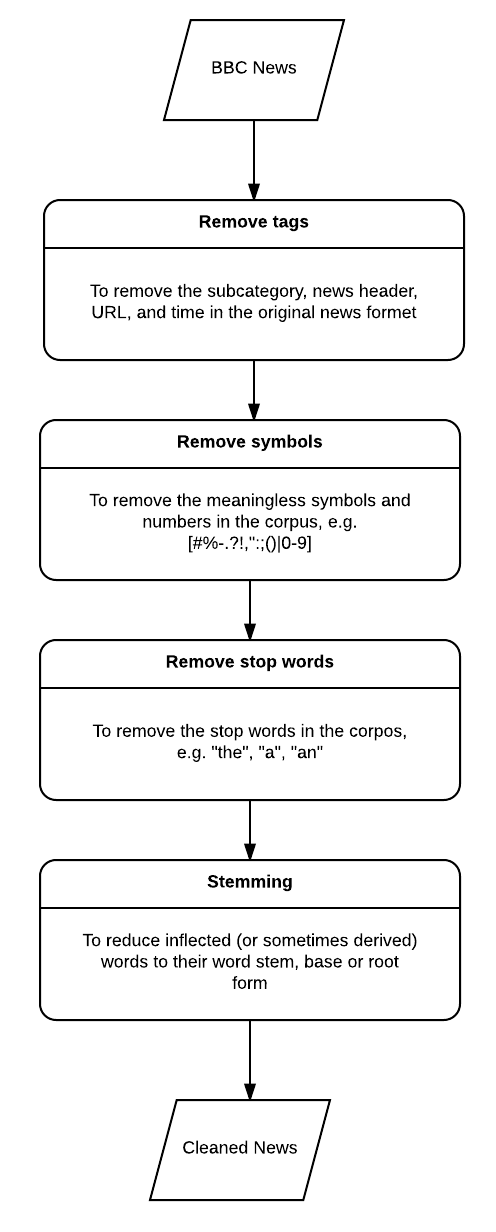
\includegraphics[width=0.5\textwidth]{figures/pipeline.png}
\caption{Preprocessing Pipeline for BBC News.}
\label{fig:pipeline}
\end{figure}

\begin{table}[h]
\centering
\begin{tabular}{l | p {10cm}}

Category & Subcategories examples\\
\hline \hline
1. UK & uk\_england;uk\_england\_essex;uk\_england\_nottingha\_shire;
uk\_scotland\_edinburgh\_east\_fife;uk\_wales\\
2. World & world\_asia\_china;world\_latin\_america;world\_us\_canada;
world\_radio\_and\_tv\\
3. Business & business\_your\_money;business \\
4. Politics & election\_england;election\_us \\
5. Tech & technology \\
6. Science & science\_environment\\
7. Heath & health  \\
8. Education & education \\
9. Entertainment \& Arts & entertainment\_arts \\
\hline
\end{tabular}
\caption{BBC News Category and examples of subcategories}
\label{tab:news_category}
\end{table}

Statistically, we have calculated the \textit{word count} , indicating how many times a certain word token appears in the whole news corpus, and also \textit{file count}, indicating a certain word token has occurred in how many different news. 
Both of \textit{word count} and \textit{file count} follow the long tail distribution \cite{feldmann1997fitting}. Specifically, for \textit{word count}, 51\% of the total word tokens appears less than 20 times in the whole corpus, with the top 10 popular words as shown in Table ~\ref{wordcount}.
\begin{table}[h!]
\centering
 \begin{tabular}{||c c||} 
 \hline
 Word & Word Count Occurrence \\ [0.5ex] 
 \hline\hline
  police	& 22587 \\
govern	& 	19257\\
work	& 	18185\\
could	& 	15619\\
uk	& 	15386\\
report		& 14995\\
first	& 	14555\\
told	& 	14213\\
bbc		& 14046\\
make	& 	13445 \\ [1ex] 
 \hline
 \end{tabular}
 \caption{Word Count Distribution: Top 10 Popular ones}
 \label{wordcount}
\end{table}

while for \textit{file count}, 60\% of the total word token appears in less than 20 different news. the top 10 popular words as shown in Table ~\ref{filecount},

\begin{table}[h!]
\centering
 \begin{tabular}{||c c||} 
 \hline
 Word & File Count Occurrence \\ [0.5ex] 
 \hline\hline
work &	9741 \\
could &		9341\\
first &		8835\\
take &		8675\\
told &		8669\\
police	 &	8576\\
include	 &	8479\\
make &		8475\\
bbc	 &	8395\\
report	 &	8192\\ [1ex] 
 \hline
 \end{tabular}
 \caption{File Count Distribution, Top 10 Popular Ones}
 \label{filecount}
\end{table}


\section{Baselines}
We have compared our DAT model with a number of baselines which are classical algorithms. 
\begin{itemize}
    \item \textbf{Latent Dirichlet Allocation Model}: The temporal factor is not taken into consideration when classifying the news corpus as well as the author information. Related works are discussed in Section ~\ref{lda} and mathematical details for experiments are presented in \ref{4lda}
     \item \textbf{Author Topic Model}: This is a hierarchical generative model where each word
$w$ in a news is associated with two latent variables author $x$ and topic $z$. Temporal factor is not considered here. Related works are discussed in Section ~\ref{2at} and experimental setups are shown in \ref{Author-Topic model}.
      \item \textbf{Topic Tracking Model}: This is a type of dynamic topic model with considering the dependency between news in the stream. We have discussed the related literature in Section ~\ref{2tot} and how we experiment on this model in \ref{4tot}. 
\end{itemize}
In the following sections we will briefly introduce the 3 baseline models in terms of model description and experimental setups. The notations we used here can be referred in Table ~\ref{tab:notation-des}
\subsection{Latent Dirichlet Allocation Model}\label{4lda}

LDA model can be viewed as a generative model, which can be described as follows.
\begin{enumerate}
   \item For each topic $k \in [1,K]$
   \begin{enumerate}
     \item Draw a multinomial $\vec{\phi_k}$ from a Dirichlet prior $\vec{\beta}$
    \end{enumerate}
    \item For each news $m \in [1,M]$
     \begin{enumerate}
     \item Draw a multinomial $\vec{\theta_m}$ from a Dirichlet prior $\vec{\alpha}$
     
     \item For each word $n \in [1,N_m]$ in document $m$
     \begin{enumerate}
            \item Draw a topic assignment $z_{m,n}$ from per-author multinomila distribution over topic $\vec{\theta}_{m}$ %$\vec{\theta_{x_{m,n}}}$
            \item Draw a word $w_{m,n}$ from multinomial $\vec{\phi}_{z_{m, n}}$
            %$\vec{\phi_{z_{m,n}}}$
    \end{enumerate}
    \end{enumerate}
        
\end{enumerate}

Therefore the posterior distribution of the topics depends on the information from the news corpus. The parameterization of the LDA model is as follows,

\begin{eqnarray*} \label{eq:lda}
\boldsymbol{\Theta}_m | \boldsymbol{\alpha} & \sim & \text{Dirichlet}(\boldsymbol{\alpha})\\
\boldsymbol{\Phi_{k}} | \boldsymbol{\beta} & \sim & \text{Dirichlet}(\boldsymbol{\beta})\\
z_{m,n} | \boldsymbol{\Theta_{m}} & \sim & \text{Multinomial}(\boldsymbol{\Theta_{m}})\\
w_{m,n} | \boldsymbol{\Phi_{z_{m,n}}} & \sim & \text{Multinomial}(\boldsymbol{\Phi_{z_{m,n}}})\\

\end{eqnarray*}
with its graphical model representation in Figure ~\ref{fig:lda}.

\begin{figure}[h]
\centering
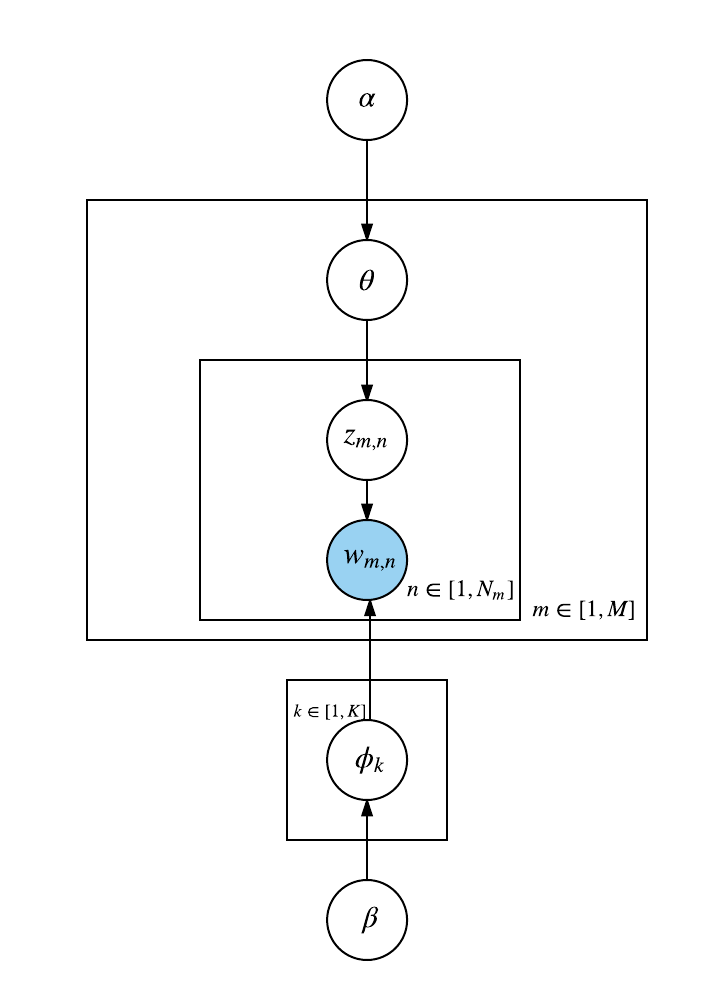
\includegraphics[width=0.6\textwidth]{figures/LDA.png}
\caption{Graphical representation of LDA topic model.}
\label{fig:lda}
\end{figure}

As discussed in ~\cite{newman2007distributed} the exact inference of LDA model is intractable, we can only employ the Gibbs sampling method as an approximate method \cite{griffiths2002gibbs}. Finally we can implement our experiments based on the way to calculate the conditional probability of the topic in ~\ref{\label{lda_z} to update the topics for each work token in each iteration. 

\begin{align}\label{lda_z}
\multicolumn{2} =   &  \math{P}({z}_{m, n}| \mathbf{w},\mathbf{z}_{\neg(m, n)},\alpha, \beta)  \nonumber
\displaybreak[3]\\ \nonumber
= & \quad \frac{\math{P}({w}_{m, n},{z}_{m, n}| \mathbf{w}_{\neg(m, n)},\mathbf{z}_{\neg(m, n)},\mathbf{x}, \alpha, \beta)}{\math{P}({w}_{m, n}| \mathbf{w}_{\neg(m, n)},\mathbf{z}_{\neg(m, n)},\mathbf{x}, \alpha, \beta)}
\displaybreak[3]\\ \nonumber
= & \quad \frac{P(\mathbf{w}, \mathbf{z} | \mathbf{x}, \alpha, \beta)}{P(\mathbf{w}, \mathbf{z}_{\neg(m,n)} |\mathbf{x}, \alpha, \beta)} \displaybreak[3]\\ \nonumber
= & \quad \frac{P(\mathbf{w}, \mathbf{z} | \mathbf{x}, \alpha, \beta)}{P(\mathbf{w}_{t,\neg(m,n)}, \mathbf{z}_{t,\neg(m,n)} | \mathbf{x},\alpha, \beta)P(w_{m,n} | \mathbf{x}, \alpha, \beta)} \displaybreak[3]\\ \nonumber
\propto & \quad \frac{P(\mathbf{w}, \mathbf{z} | \mathbf{x}, \alpha, \beta)}{P(\mathbf{w}_{\neg(m,n)}, \mathbf{z}_{\neg(m,n)} | \mathbf{x},\alpha, \beta)} \displaybreak[3]\\ \nonumber 
\propto & \quad  \left(\frac{n_{v,k}+\beta_{k,v}-1}{\sum_{v=1}^V \left(n_{v,k}+\beta_{v,k} \right)-1 } \right) \times   \left(\frac{n_{a,k}+\alpha_{k} -1}{\sum_{k=1}^K \left(n_{a,k}+\alpha_{k} \right)-1 } \right)
\displaybreak[3]\\
\end{align}

The parameter sets $\boldsymbol{\Theta}$ and $\boldsymbol{\Phi}$ can be obtained with Eqs. \ref{lda_phi} and \ref{lda_theta}.

\begin{equation}\label{lda_phi}
\phi_{k,v} = \frac{n_{k,v} + \beta_{v}}{\sum_{v=1}^V(n_{k,v} + \beta_v)}
\end{equation}

\begin{equation}\label{lda_theta}
\theta_{m,k} = \frac{n_{m,k} + \alpha_{k}}{\sum_{k=1}^K(n_{m,k} + \alpha_k)}
\end{equation}

The Gibbs sampling algorithm runs over the three periods of initialization, burn-in and sampling. The algorithm procedures that we have employed for our experiments is shown as Algorithm 2.
\begin{algorithm}\label{algo:lda}
\DontPrintSemicolon
\LinesNotNumbered
 
    \SetKwInOut{Input}{Input}
    \SetKwInOut{Output}{Output}
    \SetKwInOut{Parameter}{Global Data}

    \Input{word vector $\boldsymbol{w}$, $\alpha$,$\beta$, topic number $K$}
    \Parameter{count statistics $\{n_{m,k}\}$, $\{n_{k,v}\}$, and their sums $\{n_{m}\}$, $\{n_{k}\}$}
    \Output{topic associations $\boldsymbol{z}$, multinomila parameter $\boldsymbol{\Phi}$, and $\boldsymbol{\Theta}$}
    {// \textbf{Initialization}:}\;
    zero all count variables: $\{n_{m,k}\}$, $\{n_{k,v}\}$, $\{n_{m}\}$, $\{n_{k}\}$\;
    
    \For{all news $m \in [1,M]$ }{
      \For{all words $n \in [1,N_m]$ in news m }{
      sample topic index $z_{m,n} = k \sim \text{Multinomial}(1/K)$ \par
      increment author-topic count: $n_{m,k} += 1$\par
      increment author-topic sum: $n_{m} += 1$\par
      increment topic-word count: $n_{k,w_{m,n}} += 1$\par
      increment topic-word count: $n_{k} += 1$\par
      }
   }
   {// \textbf{Gibbs Sampling}:}\;
    sample over burn-in period and sampling period:\; 
    \caption{Inference for the LDA model using Gibbs sampling }
    \While{not finished}{
    \For{all news $m \in [1,M]$ }{
      \For{all words $n \in [1,N_m]$ in news m }{
      // For the current assignment of $k$ to the word token $w_{m,n}$ \par
      decrement author-topic count: $n_{m,k} -= 1$\par
      decrement author-topic sum: $n_{m} -= 1$\par
      decrement topic-word count: $n_{k,w_{m,n}} -= 1$\par
      decrement topic-word count: $n_{k} -= 1$\par
      sample topic index $\boldsymbol{z} \sim P(z_{m,n}|\boldsymbol{x},\boldsymbol{z}_{(\neg{m,n})},\boldsymbol{w},\boldsymbol{\alpha},\boldsymbol{\beta})$ according to Eq. \ref{lda_z}\par
      // For the new assignment of $k$ to the word token $w_{m,n}$ \par
      increment author-topic count: $n_{m,k} += 1$\par
      increment author-topic sum: $n_{m} += 1$\par
      increment topic-word count: $n_{k,w_{m,n}} += 1$\par
      increment topic-word count: $n_{k} += 1$\par
      
      }
   }
    }
    \If{converged}{
    read out parameter set $\boldsymbol{\Phi}$ according to Eq. \ref{lda_phi}\par
    read out parameter set $\boldsymbol{\Theta}$ according to Eq. \ref{lda_theta}\par
    }

\end{algorithm}


\subsection{Author-Topic Model} \label{Author-Topic model}

Author Topic model can be viewed as a hierarchical generative model, which can be described as follows,
\begin{enumerate}
   \item For each topic $k \in [1,K]$
   \begin{enumerate}
     \item Draw a multinomial $\vec{\phi_k}$ from a Dirichlet prior $\vec{\beta}$
    \end{enumerate}
   \item For each author $a \in [1,A]$
   \begin{enumerate}
     \item Draw a multinomial $\vec{\theta_a}$ from a Dirichlet prior $\vec{\alpha}$
    \end{enumerate}
    \item For each news $m \in [1,M]$
   \begin{enumerate}
     \item For each word $n \in [1,N_m]$ in document $m$
     \begin{enumerate}
            \item Draw an author $x_{m,n}$ uniformly from the group of authors $a_M$
            \item Draw a topic assignment $z_{m,n}$ from per-author multinomila distribution over topic $\vec{\theta}_{x_{m, n}}$ %$\vec{\theta_{x_{m,n}}}$
            \item Draw a word $w_{m,n}$ from multinomial $\vec{\phi}_{z_{m, n}}$
            %$\vec{\phi_{z_{m,n}}}$
    \end{enumerate}
    \end{enumerate}
        
\end{enumerate}

The posterior distribution of topics depends on the information from the news corpus and also the authors set, the parameterization of the Author-Topic model is 
\begin{eqnarray*} \label{eq:at}
\boldsymbol{\Theta}_a | \boldsymbol{\alpha} & \sim & \text{Dirichlet}(\boldsymbol{\alpha})\\
\boldsymbol{\Phi_{k}} | \boldsymbol{\beta} & \sim & \text{Dirichlet}(\boldsymbol{\beta})\\
z_{m,n} | \boldsymbol{\Theta_{x_{m,n}}} & \sim & \text{Multinomial}(\boldsymbol{\Theta_{x_{m,n}}})\\
w_{m,n} | \boldsymbol{\Phi_{z_{m,n}}} & \sim & \text{Multinomial}(\boldsymbol{\Phi_{z_{m,n}}})\\
x_{m,n} | A_m & \sim & \text{Multinomial}(1/A_m)\\

\end{eqnarray*}

Using the graphical model, the AT model can be shown as in Figure ~\ref{fig:at}. The inference of the model is done by Gibbs sampling.As dicussed in ~\cite{rosen2010learning}, the conditional probability of the topic and author for sampling in each iteration is shown in Eqs. ~\ref{at_x} and ~\ref{at_z}.
\begin{figure}[h]
\centering
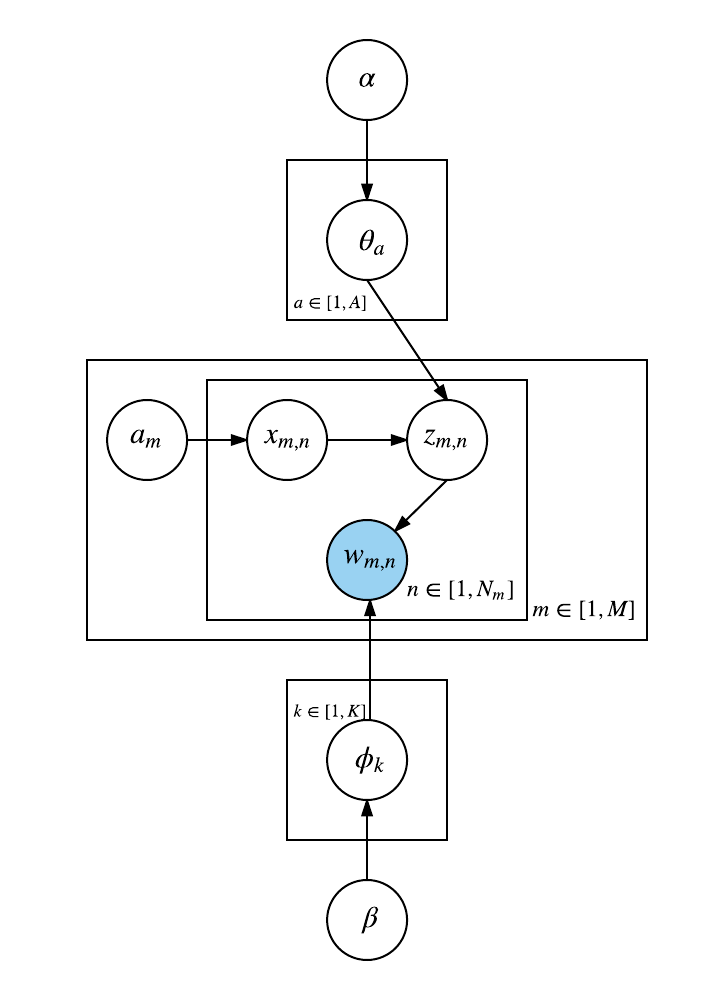
\includegraphics[width=0.6\textwidth]{figures/AT.png}
\caption{Graphical representation of Author-Topic model.}
\label{fig:at}
\end{figure}

\begin{align}\label{at_z}
\multicolumn{2} =   &  \math{P}({z}_{m, n}| \mathbf{w},\mathbf{z}_{\neg(m, n)},\mathbf{x},\alpha, \beta)  \nonumber
\displaybreak[3]\\ \nonumber
= & \quad \frac{\math{P}({w}_{m, n},{z}_{m, n}| \mathbf{w}_{\neg(m, n)},\mathbf{z}_{\neg(m, n)},\mathbf{x}, \alpha, \beta)}{\math{P}({w}_{m, n}| \mathbf{w}_{\neg(m, n)},\mathbf{z}_{\neg(m, n)},\mathbf{x}, \alpha, \beta)}
\displaybreak[3]\\ \nonumber
= & \quad \frac{P(\mathbf{w}, \mathbf{z} | \mathbf{x}, \alpha, \beta)}{P(\mathbf{w}, \mathbf{z}_{\neg(m,n)} |\mathbf{x}, \alpha, \beta)} \displaybreak[3]\\ \nonumber
= & \quad \frac{P(\mathbf{w}, \mathbf{z} | \mathbf{x}, \alpha, \beta)}{P(\mathbf{w}_{t,\neg(m,n)}, \mathbf{z}_{t,\neg(m,n)} | \mathbf{x},\alpha, \beta)P(w_{m,n} | \mathbf{x}, \alpha, \beta)} \displaybreak[3]\\ \nonumber
\propto & \quad \frac{P(\mathbf{w}, \mathbf{z} | \mathbf{x}, \alpha, \beta)}{P(\mathbf{w}_{\neg(m,n)}, \mathbf{z}_{\neg(m,n)} | \mathbf{x},\alpha, \beta)} \displaybreak[3]\\ \nonumber 
\propto & \quad  \left(\frac{n_{v,k}+\beta_{k,v}-1}{\sum_{v=1}^V \left(n_{v,k}+\beta_{v,k} \right)-1 } \right) \times   \left(\frac{n_{a,k}+\alpha_{k} -1}{\sum_{k=1}^K \left(n_{a,k}+\alpha_{k} \right)-1 } \right)
\displaybreak[3]\\
\end{align}
 
\begin{align}\label{at_x}
\multicolumn{2} =   &  \math{P}({x}_{m, n}| \mathbf{z},\mathbf{x}_{\neg(m, n)}, \mathbf{a},\alpha) \nonumber
\displaybreak[3]\\ \nonumber
= & \quad \frac{\math{P}({x}_{m, n},{z}_{m, n}| \mathbf{x}_{\neg(m, n)},\mathbf{z}_{\neg(m, n)}, \mathbf{a},\alpha)}{\math{P}({z}_{m, n}| \mathbf{x}_{\neg(m, n)},\mathbf{z}_{\neg(m, n)}, \mathbf{a},\alpha)}
\displaybreak[3]\\ \nonumber
= & \quad \frac{P(\mathbf{x}, \mathbf{z} | \mathbf{a}, \alpha)}{P(\mathbf{z}, \mathbf{x}_{\neg(m,n)} | \mathbf{a},\alpha)} \displaybreak[3]\\ \nonumber
= & \quad \frac{P(\mathbf{x}, \mathbf{z} | \mathbf{a}, \alpha)}{P(\mathbf{x}_{\neg(m,n)}, \mathbf{z}_{\neg(m,n)} | \alpha, \mathbf{a})P(z_{m,n} |  \alpha, \mathbf{a})} \displaybreak[3]\\ \nonumber
= & \quad \frac{P(\mathbf{x}, \mathbf{z} | \mathbf{a}, \alpha)}{P(\mathbf{x}_{\neg(m,n)}, \mathbf{z}_{\neg(m,n)} | \alpha, \mathbf{a})} \displaybreak[3]\\ \nonumber
%
\propto & \quad   \left(\frac{n_{a,k}+\alpha_{k} -1}{\sum_{k=1}^K \left(n_{a,k}+\alpha_{k} \right)-1 } \right)
\displaybreak[3]\\
\end{align}

By calculating the expectation of the Dirichlet distribution of $\boldsymbol{\Theta}$ and $\boldsymbol{\Phi}$ we can obtain the update rule as in Eqs. ~\ref{at_phi} and ~\ref{at_theta}:


\begin{equation}\label{at_phi}
\phi_{k,v} = \frac{n_{k,v} + \beta_{v}}{\sum_{v=1}^V(n_{k,v} + \beta_v)}
\end{equation}

\begin{equation}\label{at_theta}
\theta_{a,k} = \frac{n_{a,k} + \alpha_{k}}{\sum_{k=1}^K(n_{a,k} + \alpha_k)}
\end{equation}

In Algorithm 3 we show how we employ our inference algorithm for Author Topic model for the experiments. 


\begin{algorithm}\label{algo:AT}
\DontPrintSemicolon
\LinesNotNumbered
 
    \SetKwInOut{Input}{Input}
    \SetKwInOut{Output}{Output}
    \SetKwInOut{Parameter}{Global Data}

    \Input{word vector $\boldsymbol{w}$, author vector $\boldsymbol{a}$, $\alpha$,$\beta$, topic number $K$}
    \Parameter{count statistics $\{n_{a,k}\}$, $\{n_{k,v}\}$, and their sums $\{n_{a}\}$, $\{n_{k}\}$}
    \Output{topic associations $\boldsymbol{z}$, author associations $\boldsymbol{a}$, multinomila parameter $\boldsymbol{\Phi}$, and $\boldsymbol{\Theta}$}
    {// \textbf{Initialization}:}\;
    zero all count variables: $\{n_{a,k}\}$, $\{n_{k,v}\}$, $\{n_{a}\}$, $\{n_{k}\}$\;
    
    \For{all news $m \in [1,M]$ }{
      \For{all words $n \in [1,N_m]$ in news m }{
      sample topic index $z_{m,n} = k \sim \text{Multinomial}(1/K)$ \par
      sample author index $x_{m,n} = a \sim \text{Multinomial}(1/A_m)$ \par
      increment author-topic count: $n_{a,k} += 1$\par
      increment author-topic sum: $n_{a} += 1$\par
      increment topic-word count: $n_{k,w_{m,n}} += 1$\par
      increment topic-word count: $n_{k} += 1$\par
      }
   }
   {// \textbf{Gibbs Sampling}:}\;
    sample over burn-in period and sampling period:\; 
    \caption{Inference for the Author-Topic model using Gibbs sampling }
    \While{not finished}{
    \For{all news $m \in [1,M]$ }{
      \For{all words $n \in [1,N_m]$ in news m }{
      // For the current assignment of $k$ and $a$ to the word token $w_{m,n}$ \par
      decrement author-topic count: $n_{a,k} -= 1$\par
      decrement author-topic sum: $n_{a} -= 1$\par
      decrement topic-word count: $n_{k,w_{m,n}} -= 1$\par
      decrement topic-word count: $n_{k} -= 1$\par
      sample author index $\boldsymbol{a} \sim P(x_{m,n}|\boldsymbol{x}_{(\neg{m,n})},\boldsymbol{z},\boldsymbol{a},\boldsymbol{\alpha})$ according to Eq. \ref{at_x} \par
      sample topic index $\boldsymbol{z} \sim P(z_{m,n}|\boldsymbol{x},\boldsymbol{z}_{(\neg{m,n})},\boldsymbol{w},\boldsymbol{\alpha},\boldsymbol{\beta})$ according to Eq. \ref{at_z}\par
      // For the new assignment of $k$ and $a$ to the word token $w_{m,n}$ \par
      increment author-topic count: $n_{a,k} += 1$\par
      increment author-topic sum: $n_{a} += 1$\par
      increment topic-word count: $n_{k,w_{m,n}} += 1$\par
      increment topic-word count: $n_{k} += 1$\par
      
      }
   }
    }
    \If{converged}{
    read out parameter set $\boldsymbol{\Phi}$ according to Eq. \ref{at_phi}\par
    read out parameter set $\boldsymbol{\Theta}$ according to Eq. \ref{at_theta}\par
    }

\end{algorithm}


 
 
\subsection{Topic Tracking Model}\label{4tot}

The Topic Tracking model that we employed are based on the algorithms in \cite{liangdynamic} and \cite{iwata2009topic}. The difference of the TTM model with LDA and AT is that the news is regarded as a stream and time is taken into consideration. The generative model of TTM at time $t$ is,

\begin{enumerate}
   \item For each topic $k \in [1,K]$
   \begin{enumerate}
     \item Draw a multinomial $\vec{\phi_{t,k}}$ from a Dirichlet prior $\vec{\beta_{t,k}}\vec{\phi_{t-1,k}}$
    \end{enumerate}
    \item For each news $m \in [1,M]$
   \begin{enumerate}
   \item Draw a multinomial $\vec{\theta_{t,m}}$ from a Dirichlet prior $\vec{\alpha_t}\vec{{\theta_{t-1}}}$
     \item For each word $n \in [1,N_m]$ in document $m$
     \begin{enumerate}
            \item Draw a topic assignment $z_{m,n}$ from per-author multinomila distribution over topic $\vec{\theta_{m,t}}$ %$\vec{\theta_{x_{m,n},t}}$
            \item Draw a word $w_{m,n}$ from multinomial $\vec{\phi_{z_{m, n},t}}$
            %$\vec{\phi_{z_{m,n},t}}$
    \end{enumerate}
    \end{enumerate}
        
\end{enumerate}

The parameterization of the TTM model is as follows,
\begin{eqnarray*} \label{eq:dat}
\boldsymbol{\Theta}_{t} | \boldsymbol{\alpha_{t}}
\boldsymbol{\Theta}_{t-1}
& \sim & \text{Dirichlet}({\boldsymbol{\alpha_{a,t}}
\boldsymbol{\Theta}_{a,t-1}})\\
\boldsymbol{\Phi_{k,t}} | \boldsymbol{\beta_{k,t}}\boldsymbol{\Phi_{k,t-1}} & \sim & \text{Dirichlet}(\boldsymbol{\beta_{k,t}}\boldsymbol{\Phi_{k,t-1}})\\
z_{m,n} | \boldsymbol{\Theta_{t}} & \sim & \text{Multinomial}(\boldsymbol{\Theta_{t}})\\
w_{m,n} | \boldsymbol{\Phi_{z_{m,n},t}} & \sim & \text{Multinomial}(\boldsymbol{\Phi_{z_{m,n},t}})\\

\end{eqnarray*}

and the graphical model representation of TTM is in Figure ~\ref{fig:tot}.

\begin{figure}[h]
\centering
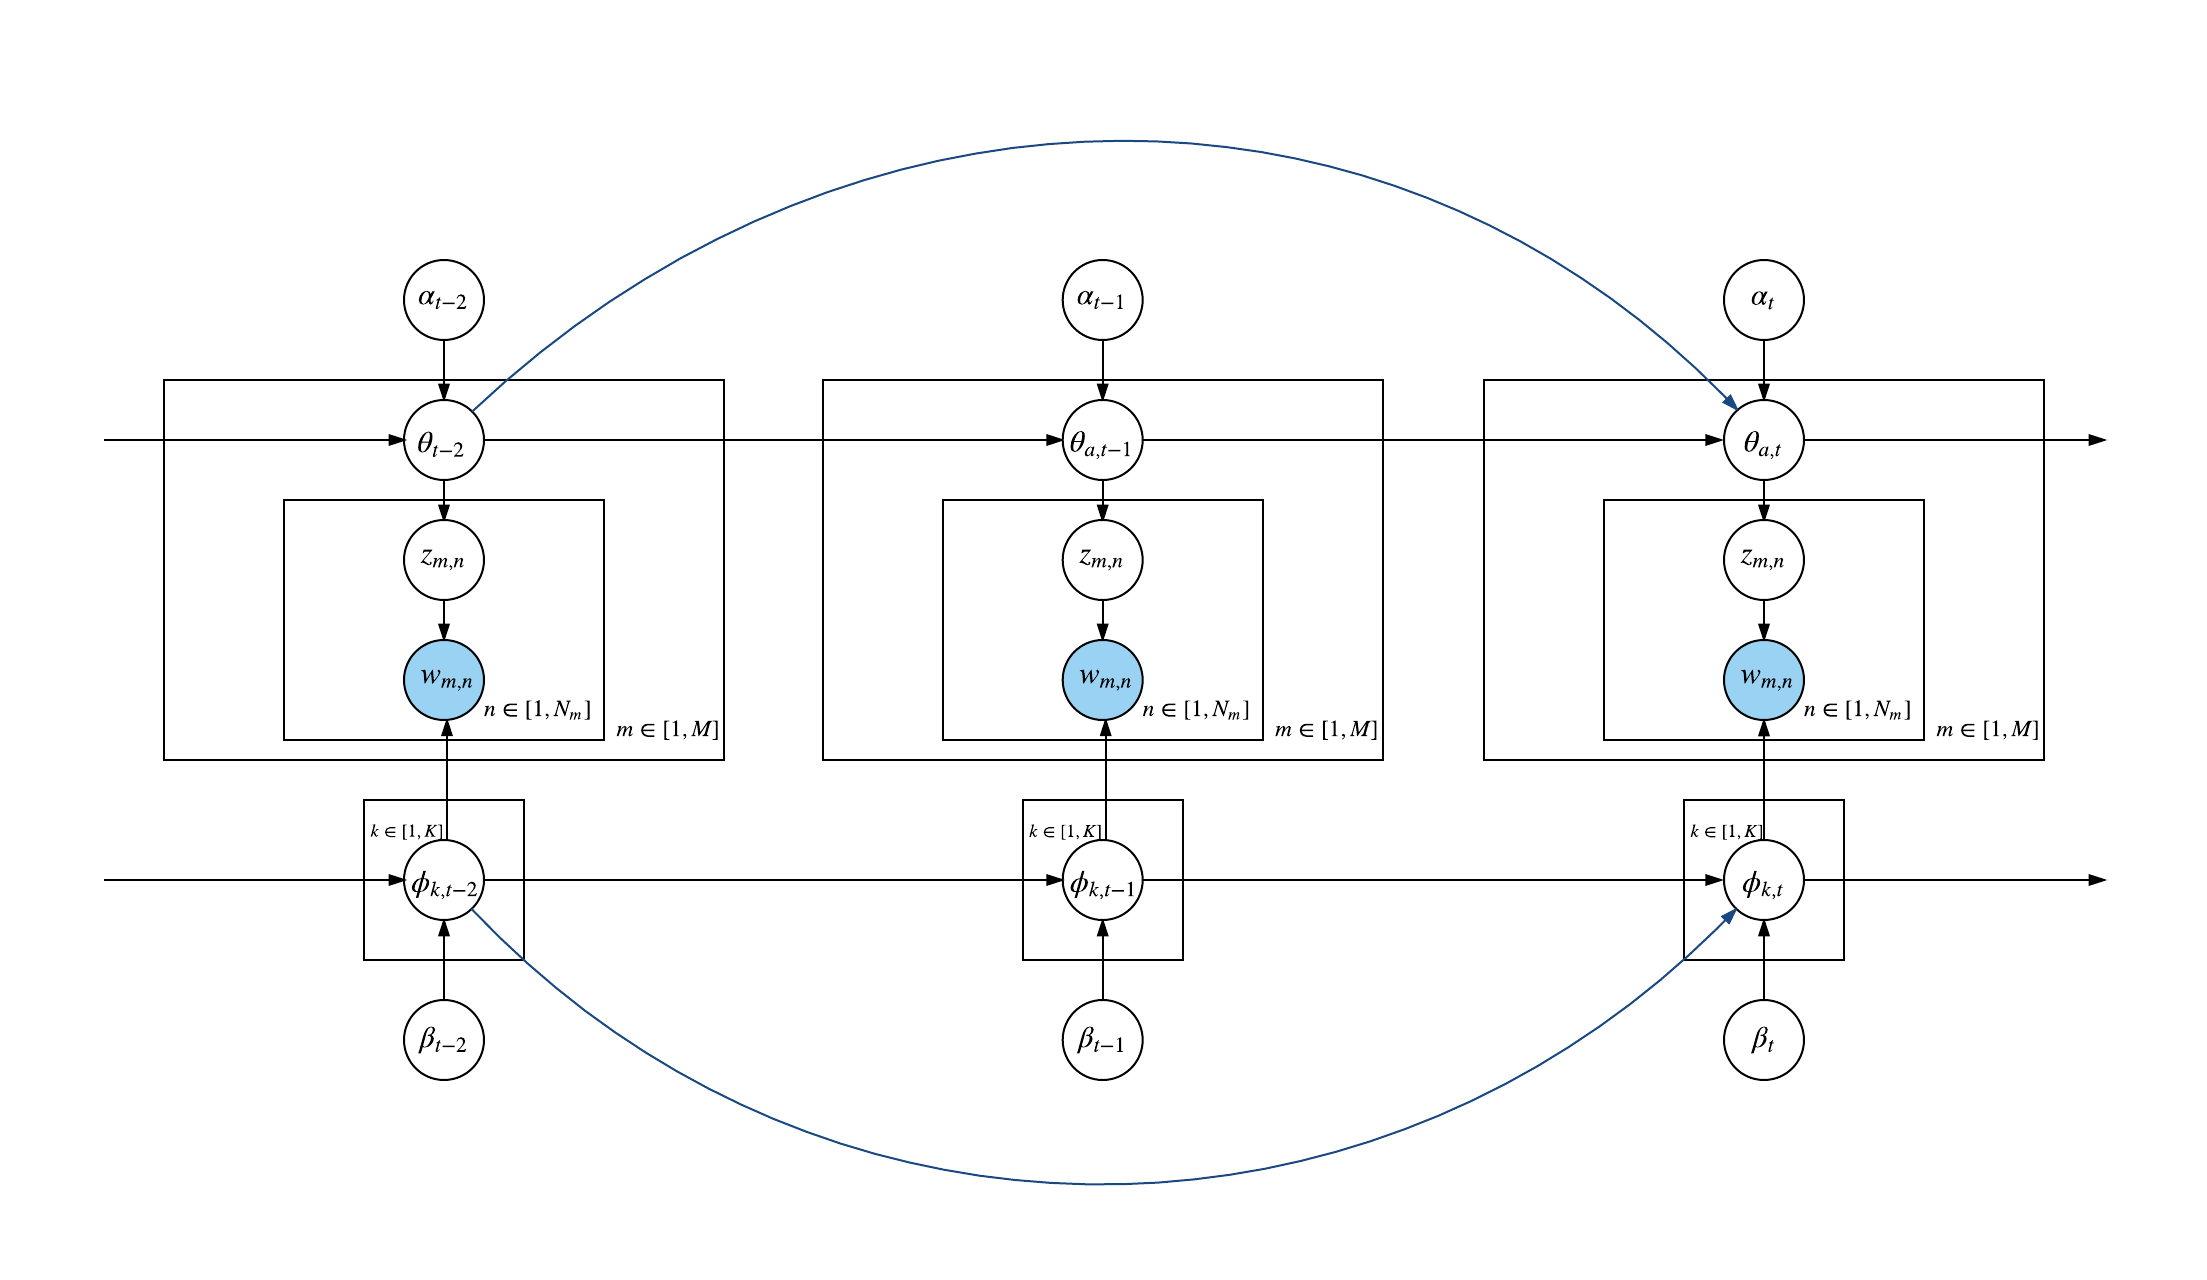
\includegraphics[width=\textwidth]{figures/TOT.png}
\caption{Graphical representation of Topic Tracking Model.}
\label{fig:tot}
\end{figure}

Similar to the inference of LDA model, the assignment of the latent topic at time $t$ can be estimated using Eqs.\ref{ttm_z}. 
\begin{align}\label{ttm_z}
\multicolumn{2} =   &  \math{P}({z}_{m, n, t}| \mathbf{w}_t,\mathbf{z}_{\neg(m, n, t)}, \alpha_t, \beta_t,\boldsymbol{\Phi}_{t-1}, \boldsymbol{\Theta}_{t-1}) \nonumber
\displaybreak[3]\\ \nonumber
\propto & \quad  \left(\frac{n_{t,v,k}+\beta_{t,k,v}\phi_{t-1}-1}{\sum_{v=1}^V \left(n_{t,v,k}+\beta_{t,v,k}\phi_{t-1} \right)-1 } \right) \times   \left(\frac{n_{t,m,k}+\alpha_{t,k} \Theta_{t-1}-1}{\sum_{k=1}^K \left(n_{t,m,k}+\alpha_{t,k}\theta_{t-1} \right)-1 } \right),
\displaybreak[3]\\
\end{align}

and by maximizing the joint distribution of topic $\boldsymbol{z}$ and word $\boldsymbol{w}$ as discussed in \cite{minka2000estimating}, we are able to obtain the update rules for the prevision values $\boldsymbol{\alpha}$ and $\boldsymbol{\beta}$ as shown in Eqs. ~\ref{tot_alpha} and \ref{tot_beta}.

\begin{equation}\label{tot_alpha}
\alpha_{t, z} \leftarrow \frac{\alpha_{t, z} \left( \Psi(m_{t, z} + \alpha_{t, z} \theta_{t-1, z}) - \Psi(\alpha_{t, z} \theta_{t-1, z}) \right)}{ \Psi(\sum_{z=1}^Z m_{t, z} + \alpha_{t, z} \theta_{t-1, z}) - \Psi(\sum_{z=1}^Z \alpha_{t, z} \theta_{t-1, z}) },
\end{equation}
%
where $\Psi(\cdot)$ defined by $\Psi(x)=\frac{\partial\log\Gamma(x)}{\partial x}$ is the digamma function; whereas the following update rule of $\beta_t$ is,
%
\begin{equation}\label{tot_beta}
\beta_{t, z, v} \leftarrow  \frac{\sum_{z=1}^Z \beta_{t, z, v} \phi_{t-1, z, v} \Psi(n_{t, z, v} +\beta_{t, z, v} \phi_{t-1, z, v}) - \Psi(\beta_{t, z, v} \phi_{t-1, z, v})}{ \sum_{z=1}^Z \phi_{t-1, z, v}  \Psi(\sum_{v=1}^V n_{t, z, v} + \beta_{t, z, v} \phi_{t-1, z, v}) - \Psi(\sum_{v=1}^V \beta_{t, z, v} \phi_{t-1, z, v})},
\end{equation}

After the iteration, the dynamic topic distribution at time $t$ can be inferred as \ref{eq:thetatz} and \ref{eq:phitzv}.

\begin{align}
\label{eq:thetatz}
\theta_{t, z}  = & \frac{ m_{t, z} + \alpha_{t, z}\theta_{t-1, z} }{ \sum_{z=1}^Z m_{t, z} + \alpha_{t, z} \theta_{t-1, z}} = \frac{ m_{t, z} + \alpha_{t, z}\theta_{t-1, z} }{ m_t + \sum_{z=1}^Z \alpha_{t, z}\theta_{t-1, z} },
%=& \frac{ m_{t, z} + \alpha_{t, z}\theta_{t-1, z} }{ m_t + \sum_z \alpha_{t, z}\theta_{t-1, z} }
\end{align}
where $m_t$ is the total number of documents in $\mathbf{d}_t$, and infer a multinomial distribution over words for topic $z$ at time $t$ as,
%
\begin{equation}
\label{eq:phitzv}
%\phi_{t, z, v} =  \frac{ n_{t, z,v } + \beta_{t, z, v} \phi_{t-1, z, v} }{ \sum_v n_{t, z, v} + \beta_{t, z, v} \phi_{t-1, z, v} } =  \frac{ n_{t, z,v } + \beta_{t, z, v} \phi_{t-1, z, v} }{ n_{t,z} + \sum_v \beta_{t, z, v} \phi_{t-1, z, v} },
\phi_{t, z, v} =  \frac{ n_{t, z,v } + \beta_{t, z, v} \phi_{t-1, z, v} }{ n_{t,z} + \sum_{v=1}^V \beta_{t, z, v} \phi_{t-1, z, v} },
%=& \frac{ n_{t, z,v } + \beta_{t, z, v} \phi_{t-1, z, v} }{ n_{t,z} + \sum_v \beta_{t, z, v} \phi_{t-1, z, v} }
\end{equation}

where $m_{t,z}$ is the number of words assigned to news $m$ at time t, $n_{t, z}$ is the number of words assigned to topic $z$ at time $t$. Whereas $m_t$ is the sum-up of $m_{t,z}$ over all topics and $n_{t, z}$ is the sum-up of $n_{t, z, v}$ over all word tokens in the news corpus. In Algorithm 4 we will show how we employ this model for our experiment.
\begin{algorithm}\label{algo:TOT}
\DontPrintSemicolon
\LinesNotNumbered
 
    \SetKwInOut{Input}{Input}
    \SetKwInOut{Output}{Output}
    \SetKwInOut{Parameter}{Global Data}

    \Input{word vector $\boldsymbol{w}$, $\alpha$,$\beta$, topic number $K$}
    \Parameter{count statistics $\{n_{m,k}\}$, $\{n_{k,v}\}$, and their sums $\{n_{m}\}$, $\{n_{k}\}$}
    \Output{topic associations $\boldsymbol{z}$, multinomila parameter $\boldsymbol{\Phi}$, and $\boldsymbol{\Theta}$}
    \If{$t=0$}{
    Set initial values for $\boldsymbol{\Theta}$ as $1/K$ and $\boldsymbol{\Phi}$ as $1/V$, also for $\boldsymbol{\alpha}$ and $\boldsymbol{\beta}$  
    }
    \For{time $t \in [1,T]$}{
    {//  
    \textbf{Initialization}:}\;
    zero all count variables: $\{n_{m,k}\}$, $\{n_{k,v}\}$, $\{n_{m}\}$, $\{n_{k}\}$\, 
    \For{all news $m \in [1,M_t]$ }{
      \For{all words $n \in [1,N_{m,t}]$ in news m }{
      sample topic index $z_{m,n} = k \sim \text{Multinomial}(1/K)$ \par
      
      increment author-topic count: $n_{m,k} += 1$\par
      increment author-topic sum: $n_{m} += 1$\par
      increment topic-word count: $n_{k,w_{m,n}} += 1$\par
      increment topic-word count: $n_{k} += 1$\par
      }
   }
   
  
   {// \textbf{Gibbs Sampling}:}\;
    sample over burn-in period and sampling period:\; 
    \caption{Inference for the Topic Tracking model model using Gibbs sampling }
    \While{not finished}{
    \For{all news $m \in [1,M_t]$ }{
      \For{all words $n \in [1,N_{m,t}]$ in news m }{
      // For the current assignment of $k$ to the word token $w_{m,n}$ \par
      decrement author-topic count: $n_{m,k} -= 1$\par
      decrement author-topic sum: $n_{m} -= 1$\par
      decrement topic-word count: $n_{k,w_{m,n}} -= 1$\par
      decrement topic-word count: $n_{k} -= 1$\par
      sample topic index $\boldsymbol{z} \sim \math{P}({z}_{m, n, t}| \mathbf{w}_t,\mathbf{z}_{\neg(m, n, t)}, \alpha_t, \beta_t,\boldsymbol{\Phi}_{t-1}, \boldsymbol{\Theta}_{t-1}) $ according to Eq. \ref{ttm_z}\par
      // For the new assignment of $k$ to the word token $w_{m,n}$ \par
      increment author-topic count: $n_{m,k} += 1$\par
      increment author-topic sum: $n_{m} += 1$\par
      increment topic-word count: $n_{k,w_{m,n}} += 1$\par
      increment topic-word count: $n_{k} += 1$\par
      
      }
   }
   Update prevision value $\boldsymbol{\alpha_t}$ according to Eq. \ref{tot_alpha}\par
    Update prevision value $\boldsymbol{\beta_t}$ according to Eq. \ref{tot_beta}\par
    }
    \If{converged}{
    Update parameter set $\boldsymbol{\Phi_t}$ according to Eq. \ref{eq:thetatz}\par
    Update parameter set $\boldsymbol{\Theta_t}$ according to Eq. \ref{eq:phitzv}\par
    
    $t= t + 1$
    }
    }
\end{algorithm}




\section{Evaluation Metrics}
\subsection{Perplexity}\label{sec:perpelexity}
Perplexity is a common  evaluation criterion for the performance of Gibbs sampler, namely when the performance of a model trained with sampling begins to level out, which means the Markov chain reaches its convergence. In our experiment we use perpelexity to assess when the performance of our model begins to stabilize, showing how good our classification of topics and authors are.
The perplexity of a set of words is defined as the exponential of negative normalized predictive likelihood under this model. Using our Dynamic Author-Topic model as an example, the perplexity of a news $m$
with length $N_m$ containing the set of the words $\boldsymbol{w_m}$ is conditioned on the known authors $\boldsymbol{a}$ of this news and also the time-frame $t$ since ours is a dynamic model. 

\begin{equation}\label{eq:perplexity0}
\mathcal L (\boldsymbol w)
    = \log p(\boldsymbol w | \boldsymbol a, t)
    = \sum_m \log p(\boldsymbol w_m | \boldsymbol a, t)
\end{equation}

Further, in our case we only have one author for each news, therefore if can be deducted as,
\begin{equation}\label{eq:perplexity0}
\begin{split}
\sum_m \log p(\boldsymbol w_m | \boldsymbol a, t)&=\sum_{t=1}^T\sum_{m=1}^{M_t} \log p(\boldsymbol w_m | \boldsymbol a, t)\displaybreak[1]\\
&=\sum_{m=1}^M \sum_{n=1}^{N_M}\log p(w | a_m, t)\displaybreak[1]\\
&=\sum_{m=1}^M \sum_{n=1}^{N_M}\log \sum_{k=1}^K p(w | t,k,a_m)p(k | t,a_m)\displaybreak[1]\\
\end{split}
\end{equation}

 In ~\ref{eq:perplexity0} it shows the log-likelihood of a set of news which contain the word sets $\boldsymbol{w}$ given the author of the news and the time if it is dynamic model. Likelihood of news can be used to compare models, higher likelihood implies a better model. Then the perplexity is traditionally used to measure the topic model, which is derived from \ref{eq:perplexity0}, as follows,
 \begin{equation}\label{eq:perplexity1}
 \text{perplexity}(\boldsymbol w) =
        \exp \left\{
        - \frac{\mathcal L(\boldsymbol w)}{\sum_{m=1}^M{N_m}}
        \right\}
\end{equation}
 
%\begin{equation}\label{eq:perplexity1}
%\text{Perplexity}(w_{m,n}|a_m) = exp(-\frac{\text{log} %p(w_{m,n}|a_m,M^\text{train})}{N_m})
%\end{equation}

From ~\ref{eq:perplexity1} we then drop the dependency of the hyperparameters $\alpha$ and $\beta$, we then approximate the integrals over $\boldsymbol{\theta}$ and $\boldsymbol{\phi}$ using the point estimation. By averaging over multiple samples we can finally obtain the probability $p(w_{m,n}|a_m,M^\text{train})$ as in formula ~\ref{eq:perplexity2},
\begin{equation}\label{eq:perplexity2}
p(w_{m,n}|a_m,M^\text{train}) \approx \frac{1}{S} \sum_{s=1}^{S}\prod_{n=1}^{N_m}[\frac{1}{A_m}\sum_{k}\theta_{a_m,k}\phi_{w_{m,n},k}|\boldsymbol{x^s},\boldsymbol{z^s},M^\text{train},\alpha,\beta]
\end{equation}

in which $A_m = 1$. 

To compute the perplexity for a whole corpus of news for Author-Topic model, based on ~\ref{eq:perplexity2} we can deduct that 

\begin{equation}\label{eq:perplexity2}
p(\boldsymbol{m}) \approx \frac{1}{S} \sum_{s=1}^{S}\prod_{n=1}^{N_m}[\frac{1}{A_m}\sum_{k}\theta_{a_m,k}\phi_{w_{m,n},k}|\boldsymbol{x^s},\boldsymbol{z^s},M^\text{train},\alpha,\beta]
\end{equation}

We will measure the perplexity based on the whole corpus, namely the collection of $\boldsymbol{w}$. Therefore, the general format of perplexity formula is inferred as follows, in which $\mathbf{m}_{\le T}$ is the collection of all news generated from time $1$ to $T$, 
\begin{equation}
\text{Perplexity}(\mathbf{m}_{\le T})=\exp\big(-\frac{ \mathcal L (\boldsymbol w)}{\sum_{t=1}^{T}\sum_{m=1}^{|\mathbf{m}_\le T|} N_{m,t}}\big)
\end{equation}

Then for different model the perplexity will be computed differently by changing $\mathcal L (\boldsymbol w)$. Specifically, for DAT model as discussed in \ref{eq:perplexity0}, it will be, 
\begin{equation}\label{p1}
\begin{split}
\mathcal L (\boldsymbol w)
    = \log p(\boldsymbol w | \boldsymbol a, t)
    = \sum_{t=1}^{T}\sum_{m=1}^{|\mathbf{m}_\le T|}\log \sum_{k=1}^K p(w | t,k,a_m)p(k | t,a_m),
\end{split}
\end{equation}
For TTM model is should be,
\begin{equation}\label{p2}
\begin{split}
\mathcal L (\boldsymbol w)
    = \log p(\boldsymbol w | \boldsymbol m, t)
    = \sum_{t=1}^{T}\sum_{m=1}^{|\mathbf{m}_\le T|}\log \sum_{k=1}^K p(w | t,k,m)p(k | t,m),
\end{split}
\end{equation}
If it is LDA model the temporal factor will not be considered, all the news in the corpus will be exchangeable, therefore we can simply ignore the time or set $T$ as 1. Then it will be, 

\begin{equation}\label{p2}
\begin{split}
\mathcal L (\boldsymbol w)
    = \log p(\boldsymbol w | \boldsymbol m)
    = \sum_{m=1}^{|\mathbf{m}|}\log \sum_{k=1}^K p(w | k,m)p(k | m),
\end{split}
\end{equation}
Similarly for AT model it is presented as follows,
\begin{equation}\label{p1}
\begin{split}
\mathcal L (\boldsymbol w)
    = \log p(\boldsymbol w | \boldsymbol a)
    = \sum_{m=1}^{|\mathbf{m}|}\log \sum_{k=1}^K p(w | k,a_m)p(k | a_m),
\end{split}
\end{equation}







\subsection{Topic Assignment}\label{sec:topicassignment}

Perplexity can be used to measure how well the word counts of the documents are represented by the word distributions represented by the topics. Perplexity is good for relative comparisons between models or parameter settings, but its real numerical value dose not have too much meaning. So intuitively we use the following methods to evaluate our model subjectively.

One obvious idea is that we can look at the news and based on the output from our result and see what topics the model assigns to them. Then we should inspect the news and the top words in the assigned topics manually. The question to answer is "Does it look like the topics really describe what the news are actually talking about?" And then we will look at the highest-likelihood words in each topic, and to answer the question, "Do they sound like they form a cohesive "topic" or just some random group of words?"

One advantage of our BBC news dataset is that as shown in ~\ref{apiformat} our raw data contains subcategory information which are strip away for model training purpose, but can be used as the label for the news to evaluate the accuracy for topic classification. 

That is, after training based on either our DAT model or the three baselines, for each news $m$ we will have a \textit{tag} which is a tuple, with a predefined category $c$, and topic obtained from the model training:
\begin{equation}
\{c_{m, i, 1 \leq i \leq 9}, z_{m, j, \leq j \leq K}\}, 
\end{equation}
in which $z_{m,j}$ is obtained by 
\begin{equation}
\max ({I_1{p(w_{m,1}|z_{m,1},m)}},{I_2{p(w_{m,2}|z_{m,2},m)}}, \ldots , {I_N{p(w_{m,N}|z_{m,N},m)}})
\end{equation}
where ${{p(w_{m,n}|z_{m,n},m)}}$ is the word distribution probability $w_{m,n}$ over topic $z_{m,n}$, and ${I_n}$ is the occurrence number of token $w_{m,n}$ in the whole news document $m$. We visualize that for each topic $z$ the category $c$ distribution in terms of articles frequecncy. This can be regarded a \textit{visual confusion matrix} is a histogram that can describe the performance of a classification model on our news data for which the category values are known \cite{townsend1971theoretical}. In order to show an even category distribution for each topic the article number actually is normalized by the minimum number of articles for the categories.


The idea is to select the topic associated the word which can mostly represent the substance of the news. Then we will investigate the co-occurrence of $c$ and $z$ on the basis of the whole news corpus, we will derive the category distribution for each topic and then select the prominence category, which should correspond to the real meaning of the topic we obtained.


\section{Setting}

The target of our experiments is to (a) evaluate the performance of Dynamic Author-Topic model with the other three baseline algorithms. (b) evaluate the performance of Dynamic Author-Topic model based on different term dependency. 

As the preparation work, the news data is processed using the pipeline introduce in Section 4.1. Our proposed model is developed based on Algorithm 1 in Section 3.3, and the other three models are implemented based on Algorithm 2,3,4 as discussed in Section 4.2. 

Then we compare the performance of DAT with each of the three baseline algorithm in terms of topic generalization and topic segmentation. Topic generalization is measured by perplexity as discussed in 4.3.1 lower perplexity means higher log-likelihood of the words over the topic, so the model is better. Topic segmentation is measured using our methodology proposed in 4.3.2. We check the co-occurrence of category and topic based on the visual confusion matrix and then manually interpret the topics based on its word distribution and double check with the news trends on BBC. 
For term dependency evaluation we have split the whole news dataset into subsets based on week, half month, and month respectively, our DAT model is running on all the three news stream, only topic distribution performance will be evaluated since the perplexities will not change a lot in the three different scenarios.

The research questions that we try to investigate in our experiment are:
\begin{description}
	\item On the basis of classification performance:
	\begin{description}
	\item[\textbf{RQ1}:] How does the proposed DAT model perform compared to baseline algorithms in terms of topic extraction? %(See Section~\ref{subsec:diversification})
	\item[\textbf{RQ2}:] How does the performance of the DAT model change with varying length of dependency time ?
	\item[\textbf{RQ3}:] How does the proposed DAT model perform in terms of topic evolution? %(See Section~\ref{})
	\item[\textbf{RQ4}:] How does the proposed DAT model perform in terms of preventing from confounding co-occurrence patterns for topic discovery? %(See Section~\ref{})
	\item[\textbf{RQ5}:] Is the performance of DAT model sensitive to the number of topics used in the model? %(See Section~\ref{}) 
	\end{description}
	\item On the basis of the generative model:
	\begin{description}
	\item[\textbf{RQ6}:] What is the performance of the generative DAT model compared to other baseline topic models in terms of the likelihood of generating the news document measured by perplexity as discussed in Section ~\ref{sec:perpelexity}?
	\end{description}
\end{description}

\chapter{Results and Analysis}
\label{chapterlabel5}
Chapter~\ref{chapterlabel4} introduces the layout of the experiment. In Chapter~\ref{chapterlabel5} the experimental results will be shown as well as the comparison with three baselines.

\section{Performance Comparison between Dynamic Author-Topic and LDA Models}\label{sec:ldadat}

In this section we will compare the performance of Dynamic Author-Topic (DAT) and LDA models. The parameters of LDA  model is set as $\alpha = 0.1$, $\beta = 0.01$.
Similarly, for DAT model the $\alpha$  is initialized as 0.1, and $\beta$ is initialized as 0.01. Besides, we set the number of author as 9.

\subsection{Perplexity}
The perplexity comparison between LDA and DAT models is shown in Figure~\ref{fig:lda_dat_perplexity}, to answer \textbf{RQ6}. A lower perplexity score indicates a better generalization performance of the model. Figure~\ref{fig:lda_dat_perplexity} shows that our DAT model performs poorer than LDA early on but with more prior information are introduced we see the cross-over point where DAT model adapts better to our news corpus. And with the increasing number of topic numbers, we observe that both model performs better while DAT is more adaptive which answers \textbf{RQ5}. The inferior performance of DAT with low number of topic number is that our author number is fixed as 9 which restrict the flexibility of topic assignment to the news, and author assignments become randomly in this case.

\begin{figure}[h]
\centering
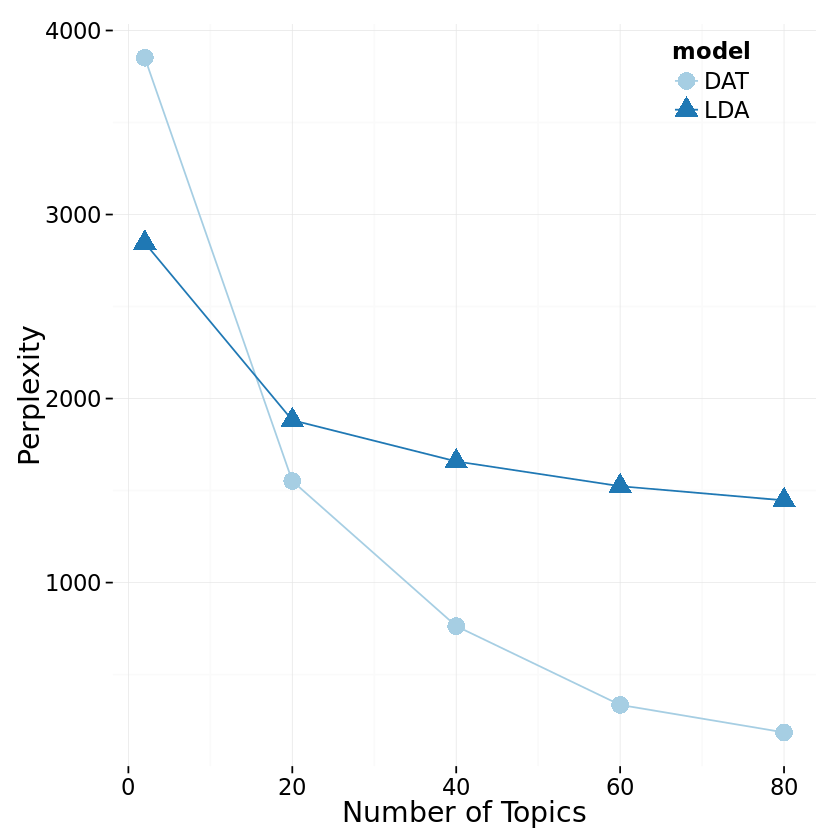
\includegraphics[width=0.7\textwidth]{figures/lda_dat_perplexity.png}
\caption{Mean perplexity of DAT and LDA with varying numbers of latent topics.}
\label{fig:lda_dat_perplexity}
\end{figure}

\subsection{Topic Distribution}\label{ldadat_td}
Here we try to evaluate the classification performance of the two model in order to answer \textbf{RQ1,3, 4}. The topic number $K$ is set as 20 here for expriment purpose. Topic- category distribution for LDA model is shown in Figure~\ref{fig:lda_with_weights} with the instruction in Section~\ref{sec:topicassignment} to evaluate the news segmentation, the facet wrap plot shows for each topic (1 to 20) how many articles are tagged with 1 of the 8 categories (the articles falling in category \textit{politics} are all also with category tag of \textit{UK} or \textit{world}, so articles with tag \textit{politics} are ignored here  ). From Figure~\ref{fig:lda_with_weights} we can observe that using LDA model the topic segmentation is prominent since for in most (18 our of 20) of the topics there is only one category dominating the tohers in terms of article number. For example, after training with LDA model, in total about 100 articles are assigned to \textit{Topic 4} which is on the upper right corner in Figure~\ref{fig:lda_with_weights}, where 62 articles are co-tagged with category \textit{entertainment} as predefined. This co-occurrence indicates that \textit{Topic 4} can be manually interpreted as \textit{entertainment}. This can be double-checked with viewing the most relevant words for each topic where appropriate shown in Table~\ref{table:ldatopicdistribution}.
\begin{figure}[h]
\centering
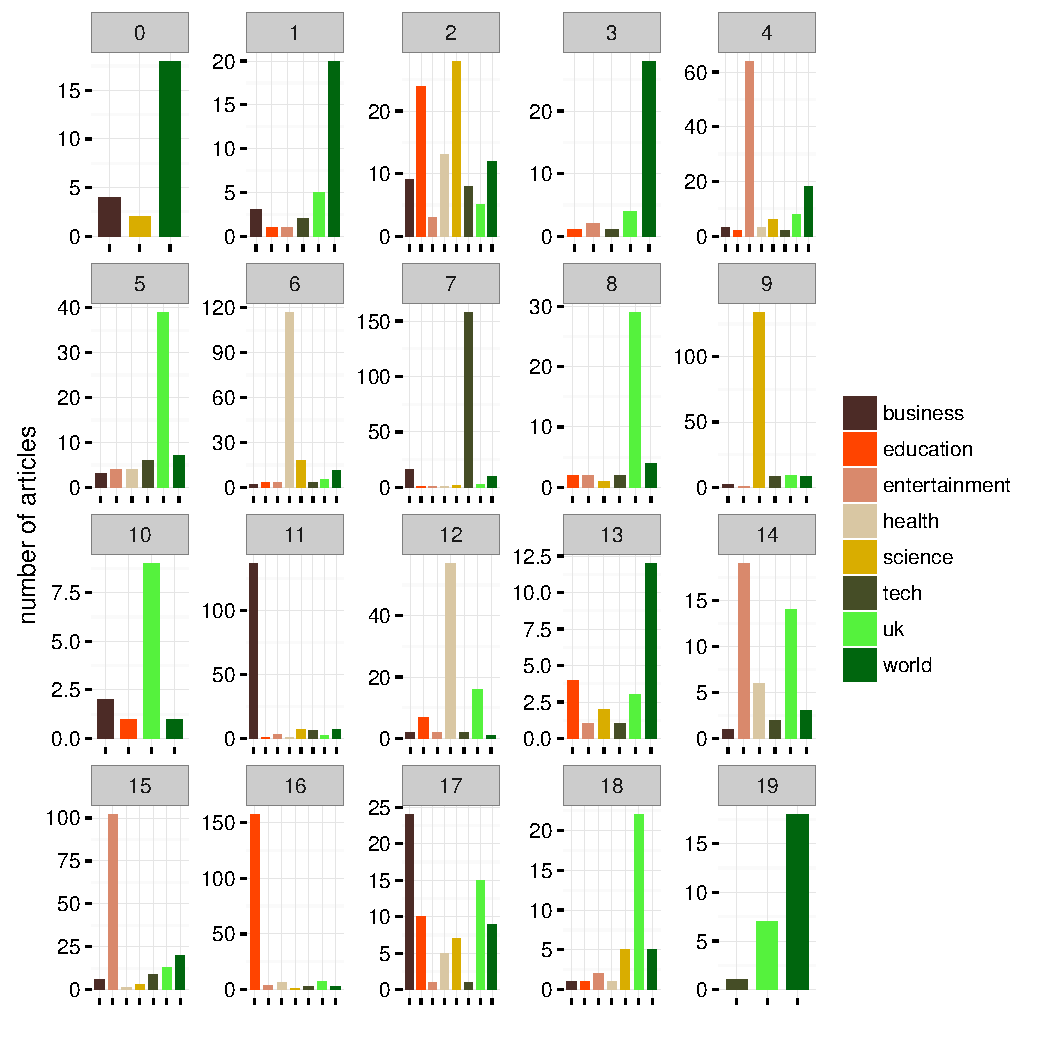
\includegraphics[width=1\textwidth]{figures/lda_with_weights.pdf}
\caption{Topic-categoy distribution of LDA model.}
\label{fig:lda_with_weights}
\end{figure}

\begin{table}[h!]
\centering
\begin{tabular}{|c c|} 
\hline
\multicolumn{2}{|c|}{\textbf{Topic 4 : Entertainment}} \\
\hline
 \textbf{WORD} & \textbf{PROB}.  \\ [0.3ex] 
 \hline
 	like  &   0.006608  \\ 
	go   &  0.004549  \\ 
	get   &  0.004535  \\ 
	bbc   &  0.004427  \\ 
	first   &  0.004388  \\ 
	show   &  0.004210  \\ 
	work   &  0.004058  \\ 
	music   &  0.003949  \\ 
	world   &  0.003945  \\ 
	day   &  0.003721  \\ 
	think  &   0.003566  \\ 
	story  &   0.003566  \\ 
	want   &  0.003407  \\ 
	many   &  0.003295  \\ 
	make   &  0.003272  \\ 
	play   &  0.003266  \\ 
	see   &  0.003152  \\ 
	look   &  0.003120  \\ 
	live   &  0.003073  \\ 
	thing  &   0.003016 \\ [1ex] 
 \hline
  
\end{tabular}
 \hfill
 \begin{tabular}{|c c|} 
\hline
\multicolumn{2}{|c|}{\textbf{Topic 6 : Health}} \\
\hline
 \textbf{WORD} & \textbf{PROB}.  \\ [0.3ex] 
 \hline
 health &   0.014923 \\
	hospital  &     0.010606 \\
	patient &      0.009591 \\
	cancer  &     0.007800 \\
	baby  &     0.006598 \\
	drug   &    0.006186 \\
	dry   &    0.006108 \\
	case   &    0.005651 \\
	medic  &     0.005632 \\
	treatment  &     0.005485 \\
	disease   &    0.005480 \\
	research   &    0.005440 \\
	women   &    0.004857 \\
	doctor  &     0.004646 \\
	risk   &    0.004567 \\
	death  &     0.004528 \\
	nhs  &     0.004405 \\
	zika  &     0.004332 \\
	cause   &    0.004243 \\
	virus   &    0.004239 \\ [1ex] 
 \hline
  
\end{tabular}
\hfill
\begin{tabular}{|c c|} 
\hline
\multicolumn{2}{|c|}{\textbf{Topic 7 : Tech}} \\
\hline
 \textbf{WORD} & \textbf{PROB}.  \\ [0.3ex] 
 \hline
 company &  0.009285 \\
	data  &   0.006523 \\
	firm   &  0.005587 \\
	could   &  0.005347 \\
	service  &   0.005159 \\
	inform  &   0.004911 \\
	bbc   &  0.004890 \\
	make   &  0.004840 \\
	user   &  0.004722 \\
	report  &   0.004550 \\
	phone  &   0.004487 \\
	online   &  0.004432 \\
	technology  &   0.004424 \\
	work   &  0.004378 \\
	secure  &   0.004328 \\
	system  &   0.004218 \\
	custom  &   0.003841 \\
	call  &   0.003841 \\
	compute  &   0.003841 \\
	facebook   &  0.003761 \\ [1ex] 
 \hline
 
 \end{tabular} 
\\[1cm]
 \begin{tabular}{|c c|} 
\hline
\multicolumn{2}{|c|}{\textbf{Topic 9 : Science}} \\
\hline
 \textbf{WORD} & \textbf{PROB}.  \\ [0.3ex] 
 \hline
 site  & 0.006374  \\ 
	project  &   0.005936  \\ 
	plan   &  0.005232  \\ 
	work   &  0.004813  \\ 
	build   &  0.004781  \\ 
	develop  &   0.004430  \\ 
	could &    0.004268  \\ 
	area  &   0.004226  \\ 
	space  &   0.004213  \\ 
	plant  &   0.003632  \\ 
	land   &  0.003531  \\ 
	first  &   0.003512  \\ 
	water   &  0.003401  \\ 
	uk   &  0.003226  \\ 
	part  &   0.003119  \\ 
	found  &   0.003074  \\ 
	animal  &  0.002915  \\ 
	energy  &   0.002863  \\ 
	world   &  0.002811  \\ 
	design   &  0.002781 \\ [1ex] 
 \hline
  
 \end{tabular}
 \hfill
 \begin{tabular}{|c c|} 
\hline
\multicolumn{2}{|c|}{\textbf{Topic 11 : Business}} \\
\hline
 \textbf{WORD} & \textbf{PROB}.  \\ [0.3ex] 
 \hline
 company  & 0.012396 \\
	price  &  0.011260\\
	market &   0.011054\\
	bank  &  0.009842\\
	business &   0.008478\\
	oil  &  0.007454\\
	share &   0.006968\\
	sale &   0.006634\\
	china &   0.006157\\
	firm  &  0.006066\\
	growth &   0.005923\\
	rate &   0.005726\\
	uk  &  0.005698\\
	economy &   0.005410\\
	month  &  0.005285\\
	report &   0.004745\\
	invest &   0.004720\\
	product &   0.004681\\
	trade &   0.004654 \\
	fall  & 0.004614 \\[1ex] 
 \hline
  
 \end{tabular}
 \hfill
 \begin{tabular}{|c c|} 
\hline
\multicolumn{2}{|c|}{\textbf{Topic 16 : Education}} \\
\hline
 \textbf{WORD} & \textbf{PROB}.  \\ [0.3ex] 
 \hline
 school  & 0.029979 \\
	children   &  0.012832 \\
	council    & 0.008763 \\
	educate    & 0.008570 \\
	teacher   &  0.008009 \\
	report   &  0.007690 \\
	pupil   &  0.007396 \\
	work   &  0.005670 \\
	parent   &  0.005087 \\
	need   &  0.005065 \\
	govern    & 0.004812 \\
	staff   &  0.004794 \\
	service  &  0.004671 \\
	support   &  0.004404 \\
	concern   &  0.004159 \\
	issue    & 0.003980 \\
	plan    & 0.003943 \\
	child   &  0.003765 \\
	primary   &  0.003743 \\
	improve   & 0.003702 \\ [1ex] 
 \hline
  
 \end{tabular}
\caption{The topic-word distribution of LDA model}
\label{table:ldatopicdistribution}
\end{table}

In Table~\ref{table:ldatopicdistribution} we have selected 6 topics to show its top 20 words with highest probabilities conditioned on the topics. The title of the topic is our manual interpretation based on Figure~\ref{fig:lda_with_weights}. It is easily to see that for each table the words are definitely relevant to the topic itself. For example, for \textit{Topic 6, health} we can see the words like \textit{hostipital, petient, cancer, drug, treatment, zika, NHS, virus}, etc. and for \textit{Topic 16, education}, we see words like \textit{school, children, teacher, staff, primary, improve}, etc, which are all type of words for \textit{education}. 

However, although the topics segmentation is clear for LDA model, we see two drawbacks with the model.
\begin{itemize}
    \item Firstly, we cannot see the trends of the news, namely how the topics rise and fall for a certain news event. Therefore we see the words for each topic is just general words spreading through the time, for example, if we look at the words for \textit{Topic 7, tech}, it is obviously that all the words are describing technology itself however it is hardly to speculate what kind of news is happening specifically.
    \item Secondly, LDA model will confound the topics between different news event. For example, for \textit{Topic 6, health}, the words \textit{drug, treatment, hospital} are related to the events that in May the NHS will not fund anti-HIV Prep drug plan~\footnote{http://www.bbc.co.uk/news/health-36421124}, while \textit{zika} and \textit{virus} are extracted from the news events of the devastating epidemic Zika virus in Africa~\footnote{http://www.bbc.co.uk/news/health-36379455}. It is not clear what news events are captured by LDA model exactly. 
\end{itemize}

Then for DAT model, we are now running the experiment based on short-term dependency with time-period as a week. In total there are 22 weeks spreading the whole corpus, we have selected 4 of them for investigation.
Topic category distribution for DAT model is shown in Figure~\ref{subfig:11dattopiccategory} (From Jan 1 to Jan 7), Figure~\ref{subfig:212dattopiccategory} (From Feb 12 to Feb 19), Figure~\ref{subfig:34dattopiccategory} (From Jan Mar 4 to Mar 11), and Figure~\ref{subfig:520dattopiccategory} (From May 20 to May 27).

Using the same way as for exploring LDA model as above, for the four different weeks we firstly find the prominence category for each topic which will be the topic's representative, and secondly we check the most relevant words associated with each topic to see whether they are valid to discover news events.


\begin{figure*}[!t]
  \centering
    \subfigure[2016.01.01 to 2016.01.07]{
    \label{subfig:11dattopiccategory} 
    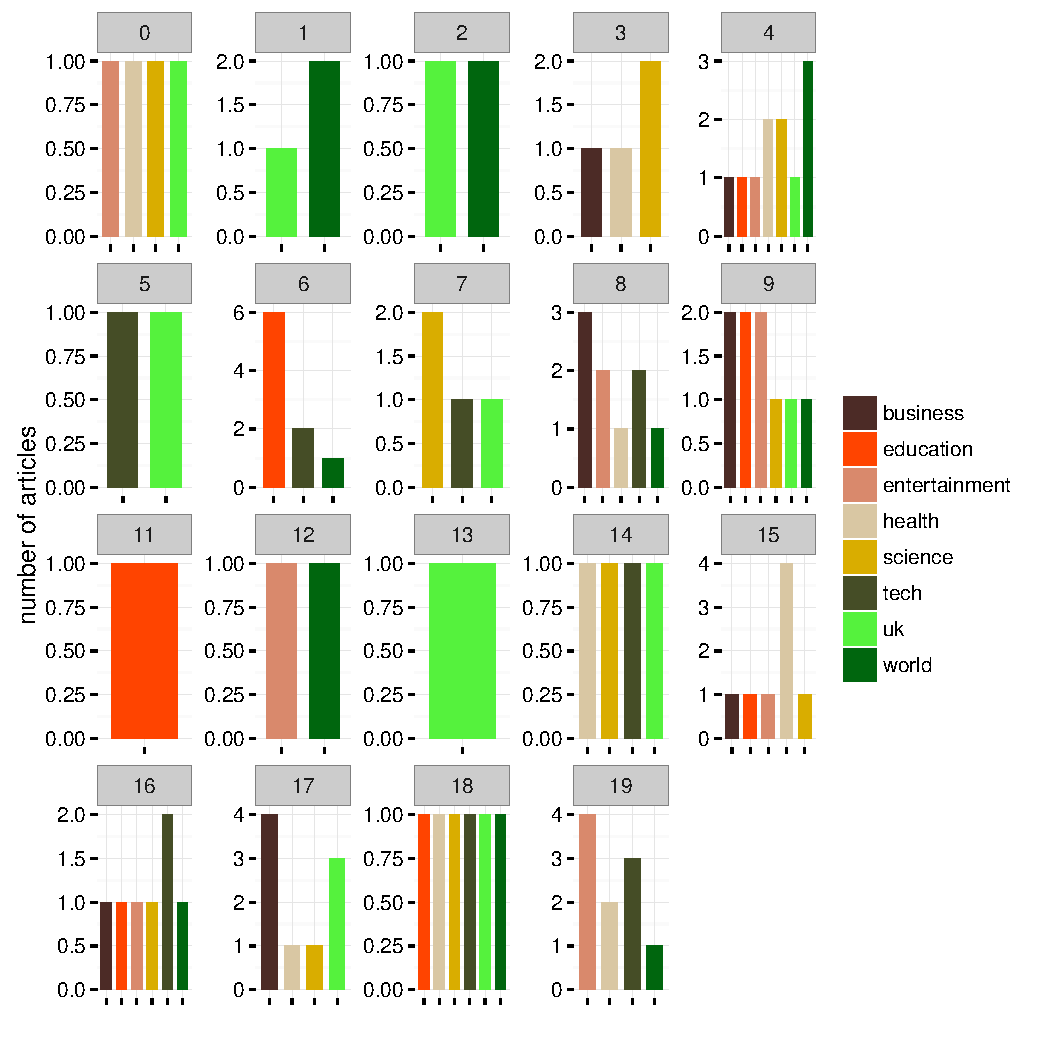
\includegraphics[width=.48\columnwidth]{figures/11datcatogery.pdf}}
    \subfigure[2016.02.12 to 2016.02.19]{
    \label{subfig:212dattopiccategory} 
    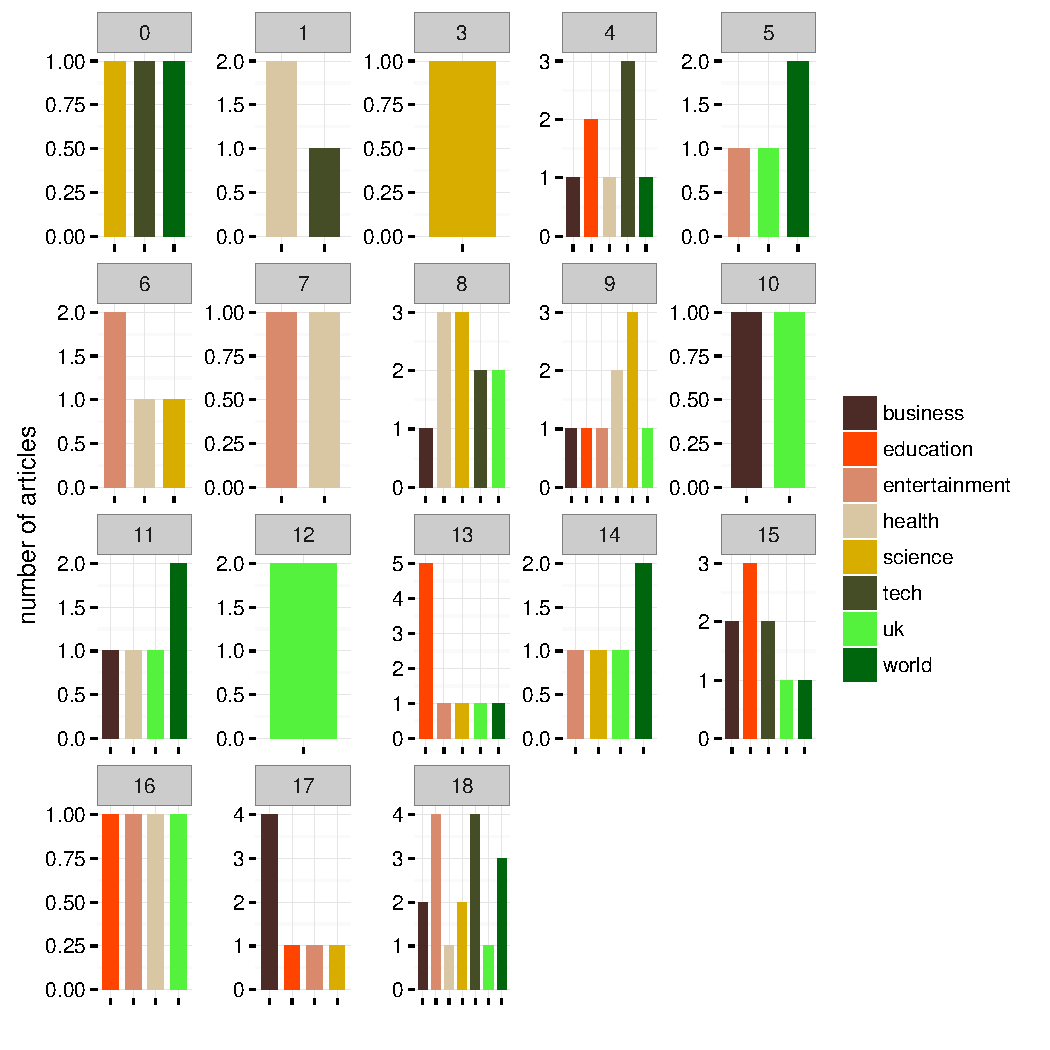
\includegraphics[width=.48\columnwidth]{figures/212datcatogery.pdf}}
    \vspace*{-.9\baselineskip}
    \subfigure[2016.03.04 to 2016.03.11]{
    \label{subfig:34dattopiccategory} 
    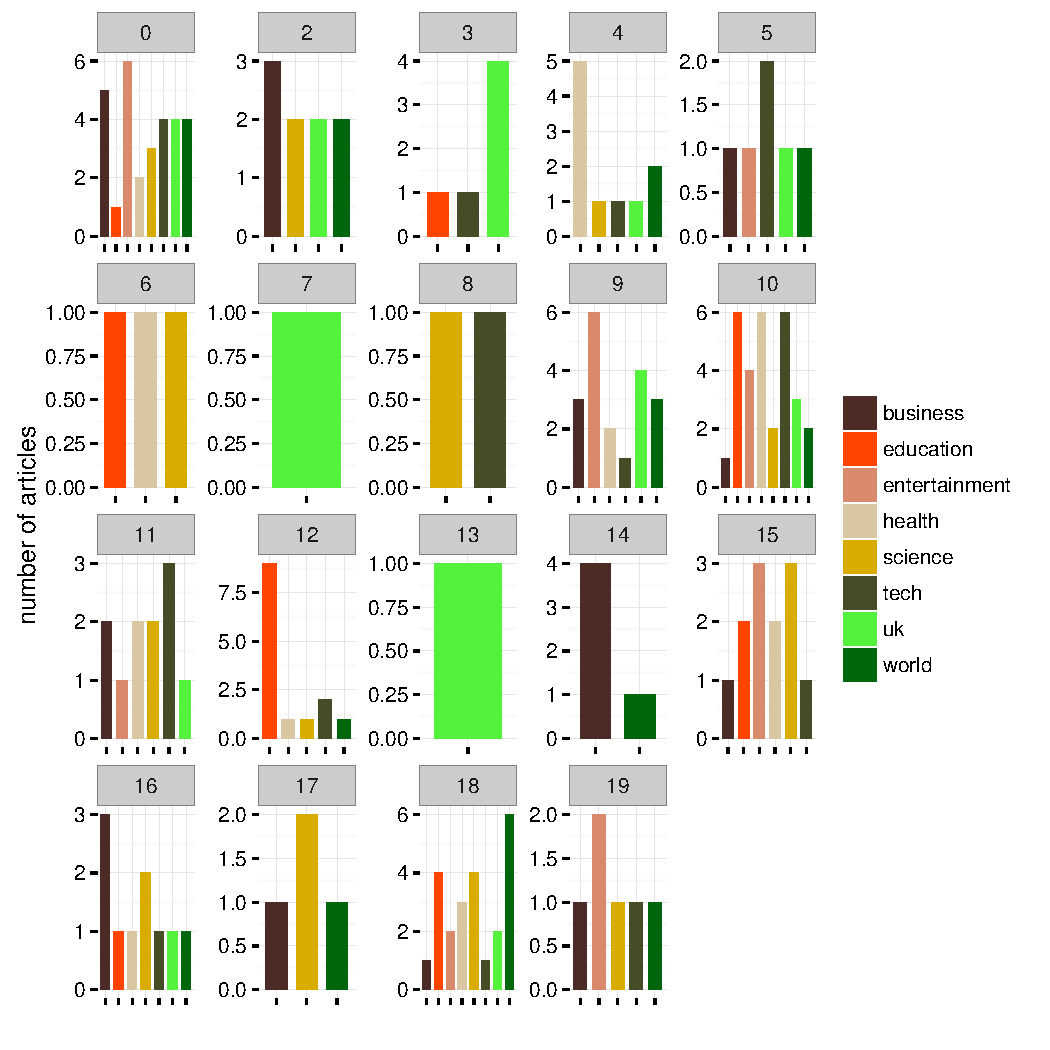
\includegraphics[width=.48\columnwidth]{figures/34datcatogery.pdf}}
    \subfigure[2016.05.20 to 2016.05.27]{
    \label{subfig:520dattopiccategory} 
    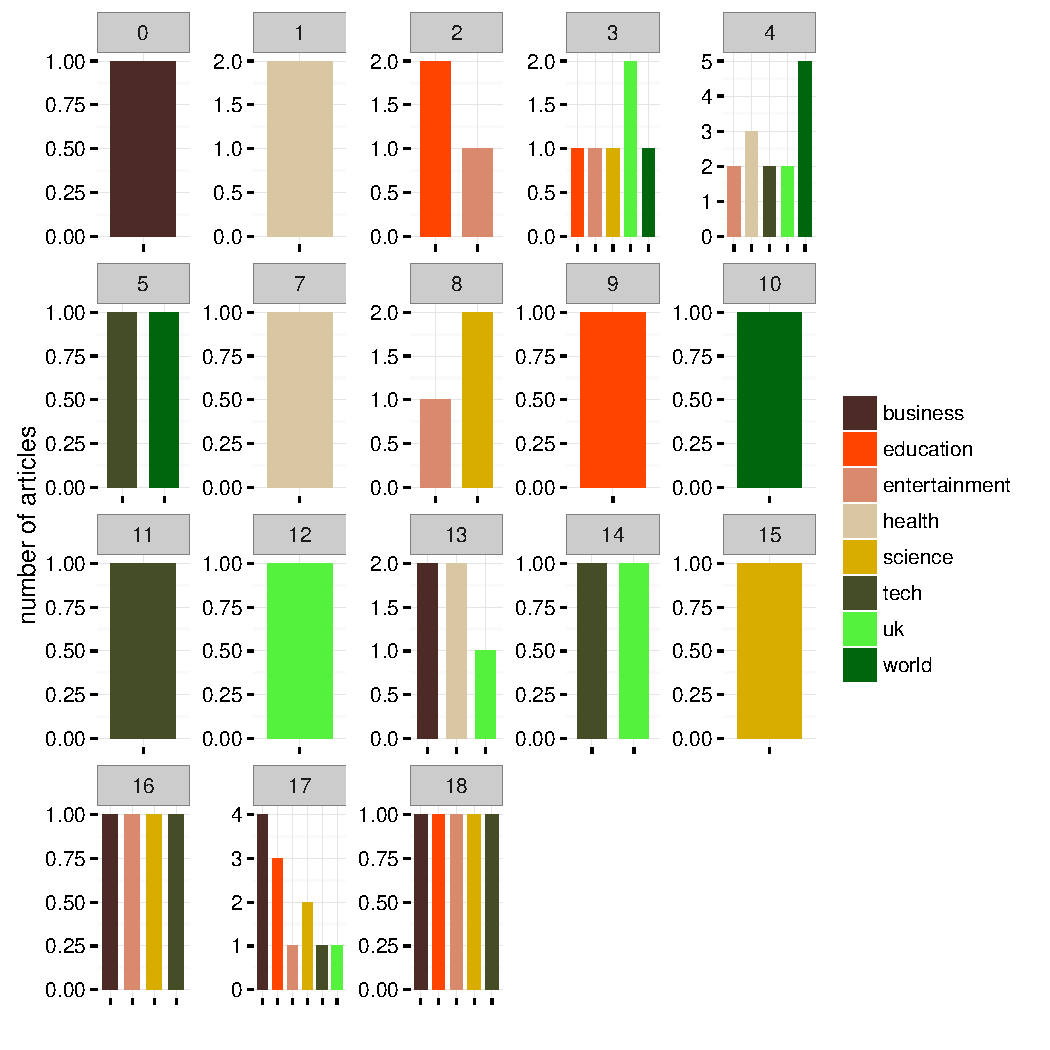
\includegraphics[width=.48\columnwidth]{figures/520datcatogery.pdf}}
\caption{\small Topic-category distribution of DAT model for 4 different weeks, which are between 2016.01.01 to 2016.01.07, between 2016.02.12 to 2016.02.19, between 2016.03.04 to 2016.03.11 and between 2016.05.20 to 2016.05.27}
\label{fig:dattopiccategory}
\end{figure*}

Let's start with the category \textit{education}, its association with different topics at different time can be interpreted with Figure~\ref{fig:dattopiccategory}. Its topic evolution can be shown as in Figure~\ref{fig:dat_education_tc}.

It shows that compared to LDA model the DAT topics are more neatly and time-related. In the week of Jan 1st, we see the words of \textit{school} which appears in most of the education news at that time. the words \textit{nation, need,expect, career} are there is due to the news that \textit{the National College of Teaching and Leadership is expecting a surge of interest in the profession of teachers}~\footnote{http://www.bbc.co.uk/news/education-35193600}. The reason you see \textit{islam} is because of the news that \textit{Trojan Horse scandal in Birmingham has been prohibited from teaching indefinitely}~\footnote{http://www.bbc.co.uk/news/education-35226482}. You see \textit{travel} and \textit{MP} because of the news that \textit{Pupils in a primary school in Yorkshire will have to travel to another school for part of each day because of difficulties in recruiting a teacher}~\footnote{http://www.bbc.co.uk/news/education-35242877}, and MPs on the Education Select Committee are warned of a deepening ``crisis" in recruiting and retaining teachers.

Then in the week of Feb 12th, we use the similar way to check DAT's performance to discover topics and prevent from confusing different event news. Since there are less than 10 news about education in this week, so it is easily to envision that the words around this topic are from the news that \textit{A flagship scheme to bring ex-servicemen and women to England's classrooms has seen 28 veterans qualify as teachers since it started}~\footnote{http://www.bbc.co.uk/news/education-35595424}, \textit{Teacher shortages mean classroom support staff are doing work normally done by qualified teachers}~\footnote{http://www.bbc.co.uk/news/education-35551009}, and some other news. 

Then in the week of Mar 4th, we can see from the words that the hot news event are \textit{Harvard Law School is to change its official seal, after a protest that it had links to slavery}~\footnote{http://www.bbc.co.uk/news/education-35726878}, and \textit{a proposal of national funding formula for schools, which would be introduced next year, would see budgets going straight to schools, removing local authorities from being a channel for funding}~\footnote{http://www.bbc.co.uk/news/education-35775458}. 

Lastly in the week of May 20th, some education news started to discuss on British EU referendum, and also the topic are also related to the news that \textit{Head teachers are calling on the education secretary to stop the publication of this year's primary school results in England.}~\footnote{http://www.bbc.co.uk/news/education-36372304}. 


\begin{figure}[h]
\centering
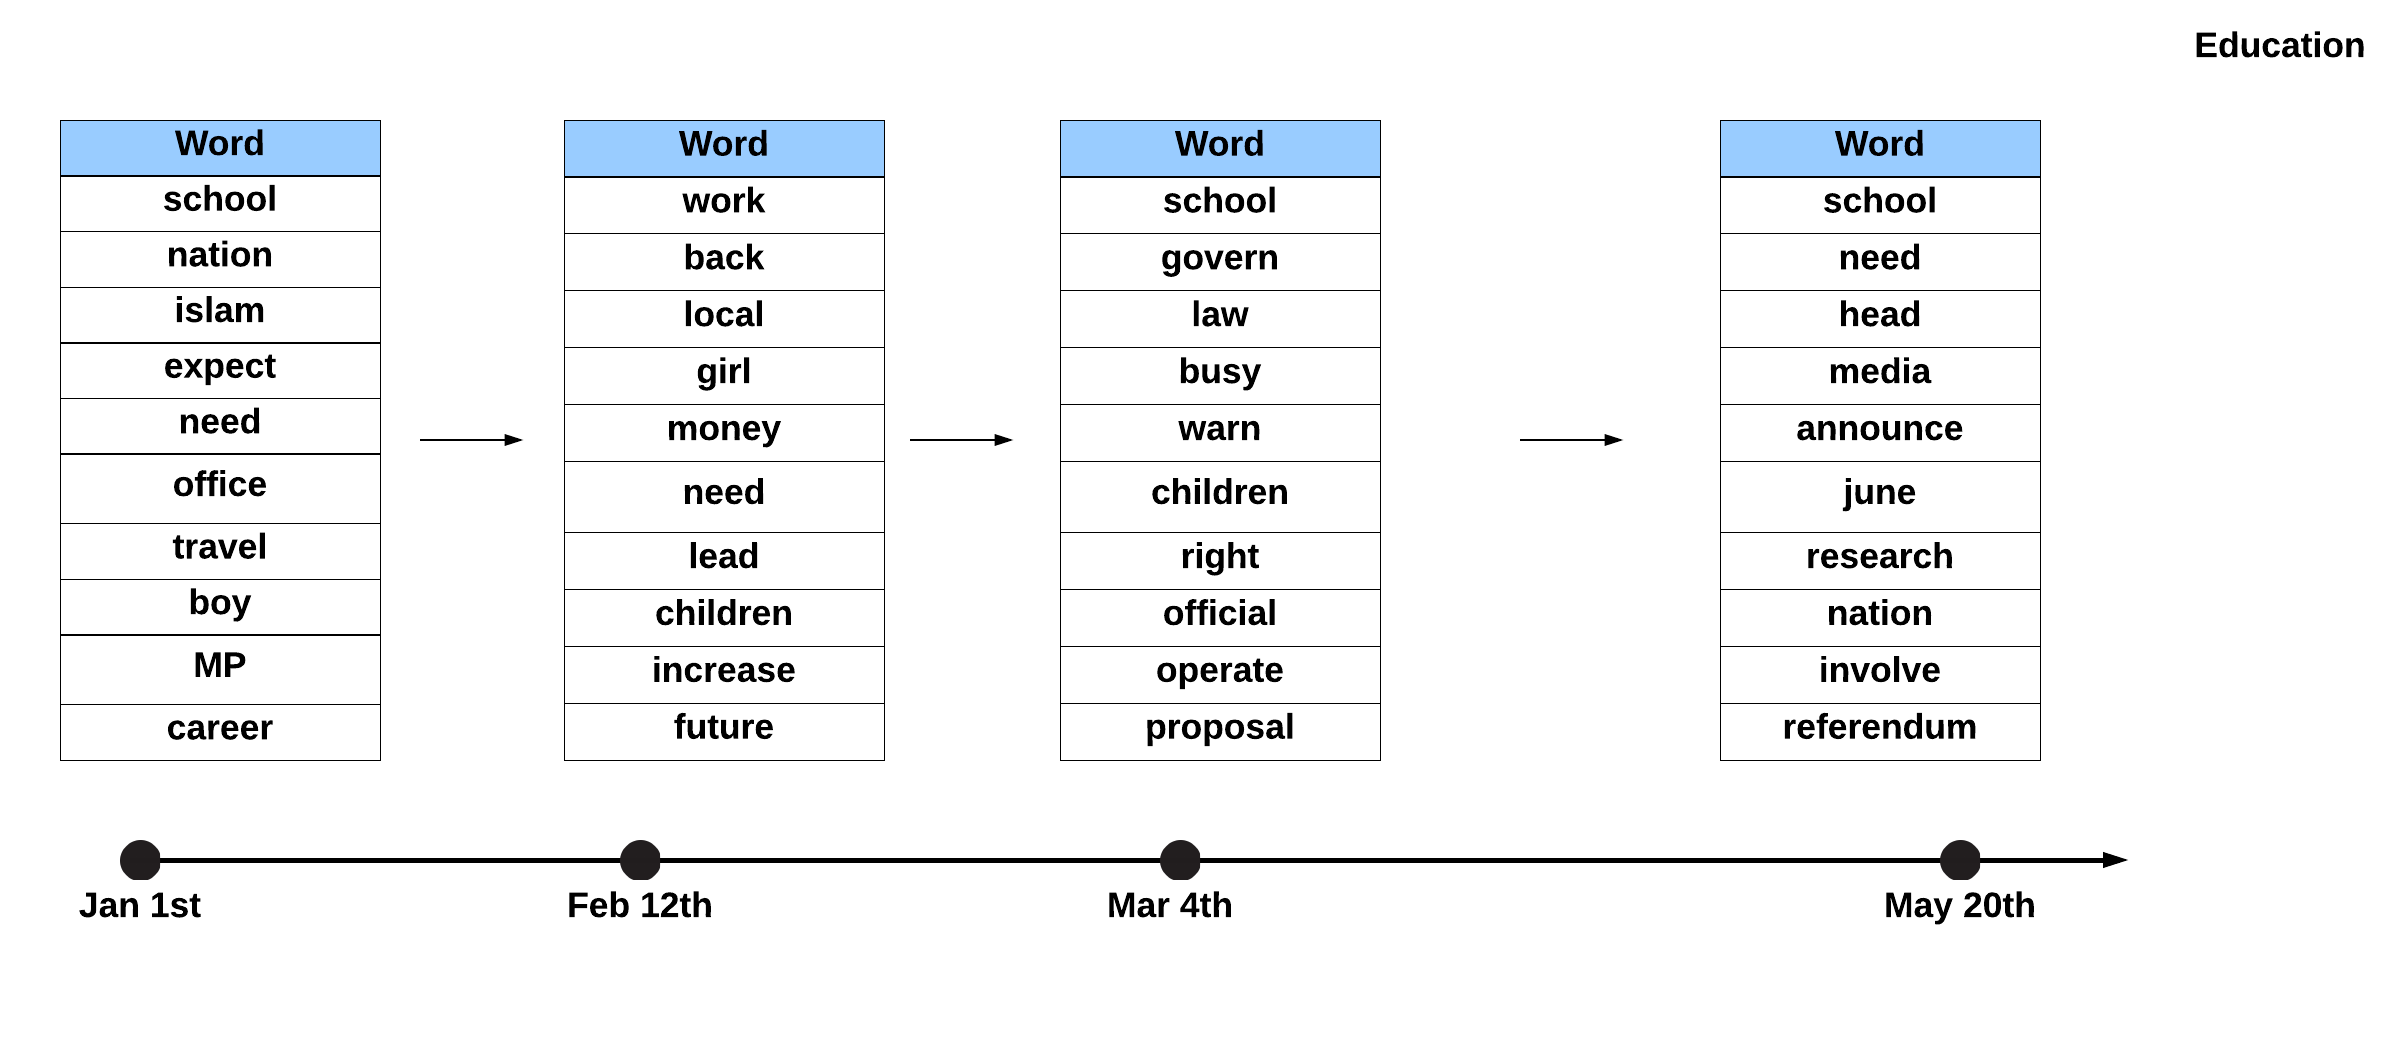
\includegraphics[width=1\textwidth]{figures/dat_education_tc.png}
\caption{Topic evolution of DAT model: use Education as an example}
\label{fig:dat_education_tc}
\end{figure}
\begin{figure}[h]
\centering
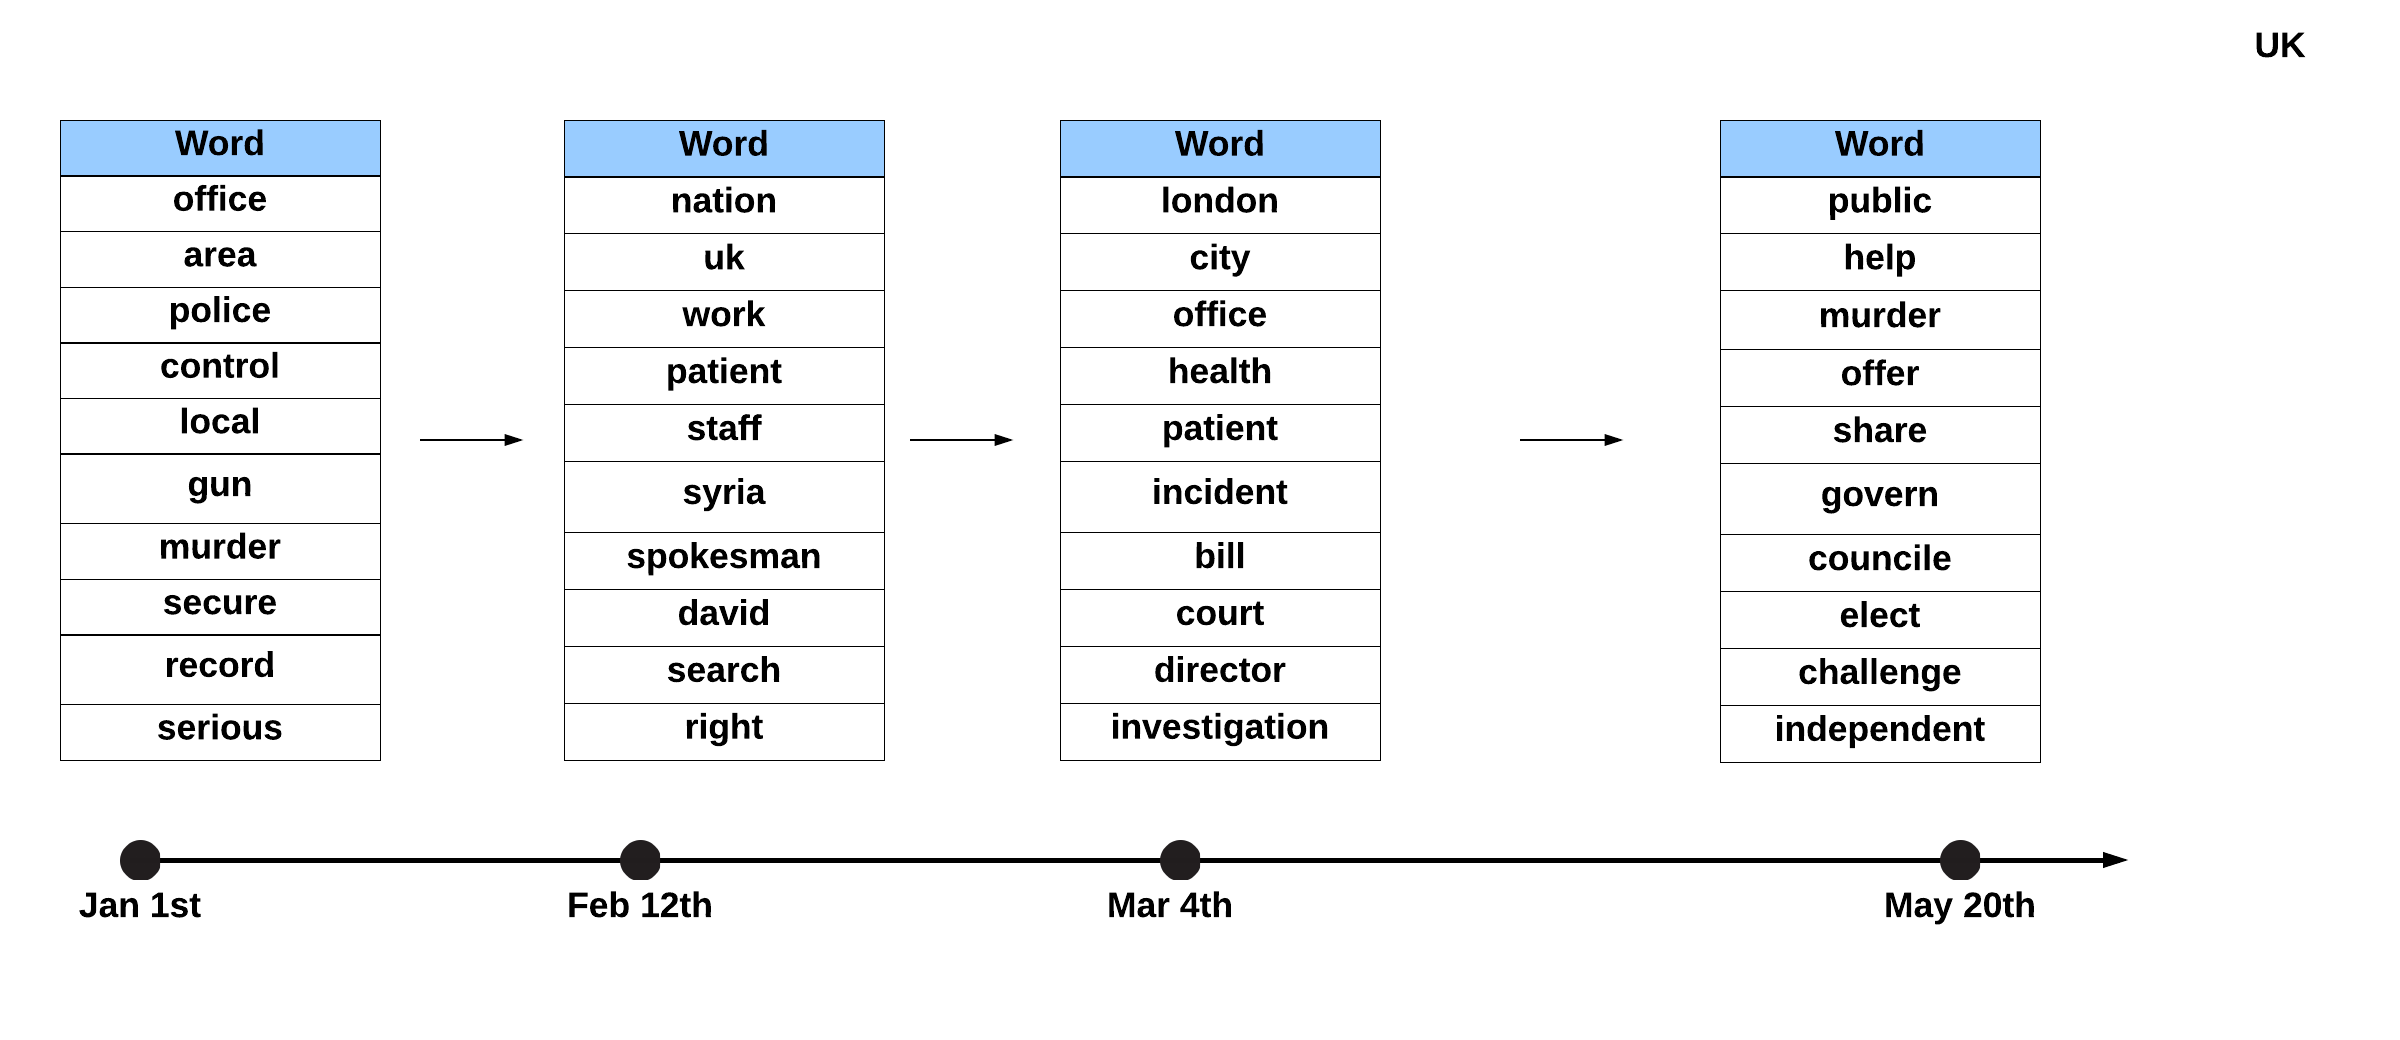
\includegraphics[width=1\textwidth]{figures/dat_uk_tc.png}
\caption{Topic evolution of DAT model: use UK as an example}
\label{fig:dat_uk_tc}
\end{figure}
\begin{figure}[h]
\centering
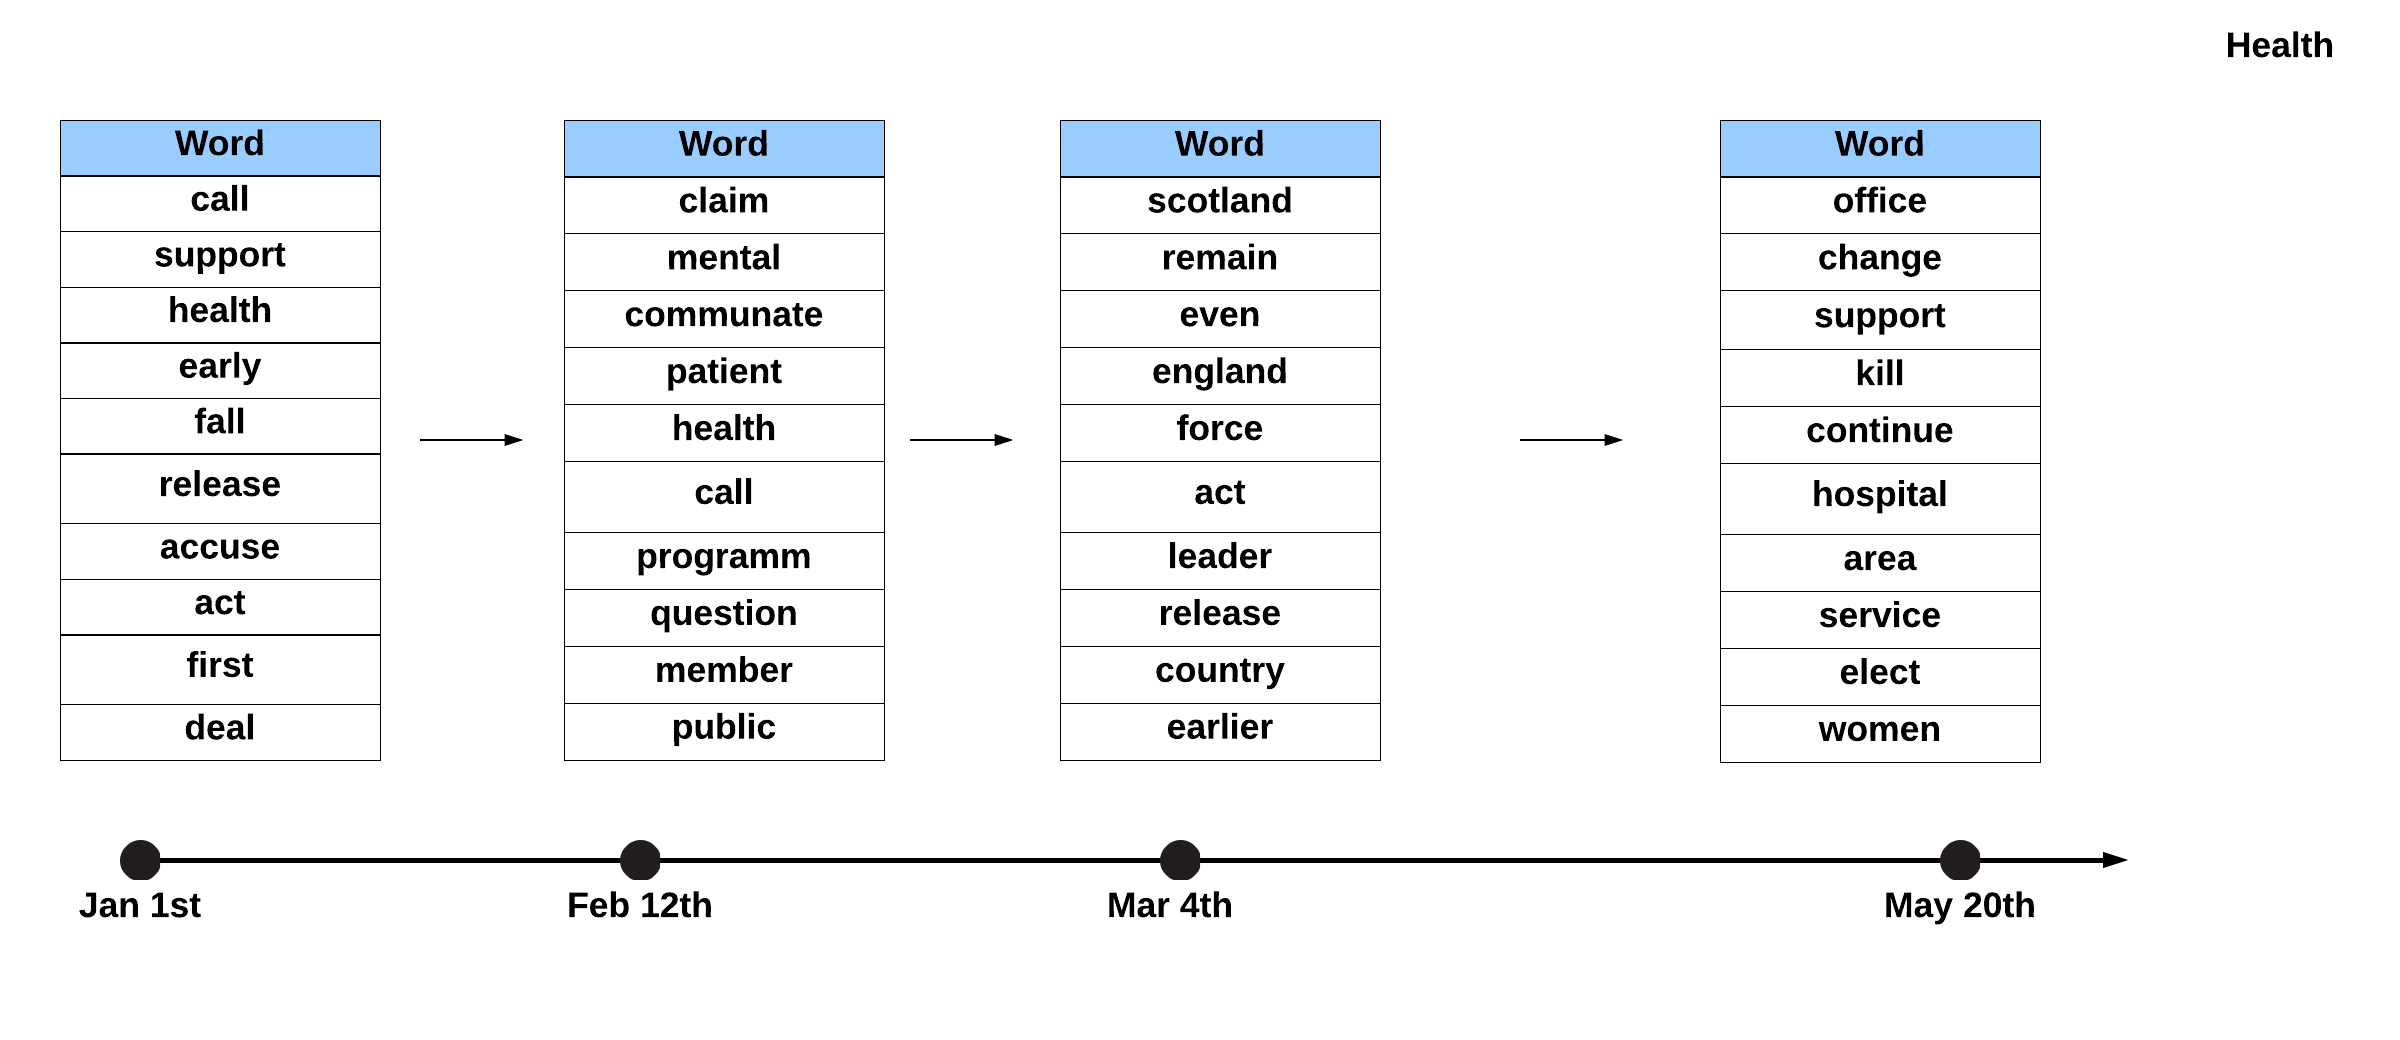
\includegraphics[width=1\textwidth]{figures/dat_health_tc.png}
\caption{Topic evolution of DAT model: use health as an example}
\label{fig:dat_health_tc}
\end{figure}

Another example we can show is for category \textit{UK}, which is presented in Figure~\ref{fig:dat_uk_tc}.

In the week of Jan 1st, quite a few news are about \textit{police, murder, secure}, such as \textit{Man arrested over murder of Daria Pionko in Leeds}~\footnote{http://www.bbc.co.uk/news/uk-england-leeds-35209489}, \textit{Pitsea stairwell death: Two men bailed by police}~\footnote{http://www.bbc.co.uk/news/uk-england-essex-35209578}, etc. Also we see record-breaking rainfall north-west England as the news discussed~\footnote{http://www.bbc.co.uk/news/uk-england-35222030}. Then in the week of Feb 12th, we see the news about \textit{UCL's research that a patient embodying themselves in a virtual reality avatar of a crying child could help with depression}~\footnote{http://www.bbc.co.uk/news/uk-35558447} and \textit{search on Ben Nevis for missing climbers}~\footnote{http://www.bbc.co.uk/news/uk-35594715} and mostly, the Syria crisis. Then when in the week of Mar 4th, one important UK news is that \textit{One of London mayoral hopeful Sadiq Khan's aides, Shueb Salar, has resigned following his suspension on Sunday}~\footnote{http://www.bbc.co.uk/news/uk-england-london-35744843}, the news that \textit{Clayton Williams tells court he `did not intend to kill officer'}~\footnote{http://www.bbc.co.uk/news/uk-35756062}, an incident at Hyder park gate~\footnote{http://www.bbc.co.uk/news/uk-england-london-35752992}, and a few investigation of criminals~\footnote{http://www.bbc.co.uk/news/uk-wales-south-east-wales-35747691}. While in the week of May 20th, we still see a few news about murder~\footnote{http://www.bbc.co.uk/news/uk-england-essex-36248166}~\footnote{http://www.bbc.co.uk/news/uk-england-36376555}~\footnote{http://www.bbc.co.uk/news/uk-england-manchester-36375040}, \textit{the news that European countries urged to improve data sharing to improve the way they gather and share information about firearms to cut gun crime}~\footnote{http://www.bbc.co.uk/news/uk-36371145}, and surely many news about election in May.

The last example is the category of \textit{health}, we only show the topic evolution here in Figure~\ref{fig:dat_health_tc}, which also uncovered the news trends among the 5 months.


The other topics also have the same pattern of changing and evolution which can indicate the rising and falling of the topics over time. Compared to LDA model, DAT's Topic-Category distribution is not as prominent as LDA model so the topic segmentation is less clear than LDA. However, DAT obviously has the advantages that it tracks the news trends and words to describe the topics are time and event specifically, unlike for LDA model the words are mostly general words which spread through the whole news corpus's time. Also DAT will not be confused by different events and is able to identify the event-specific words for the topics. An good example is that the word \textit{Islam} appears as the one of the most relevant words for topic \textit{education} on Jan 1st. Although there is no direct relation between them however since there is a news about prohibiting Trojan Horse scandal which is hotly discussed so \textit{Islam} becomes relevant to \textit{education} in this special case.

Therefore to answer \textbf{RQ1} LDA outperforms DAT, and DAT is better for \textbf{RQ3,4} and \textbf{6}.


\section{Performance Comparison between Dynamic Author-Topic and Author-Topic Models}

In this section we will compare the performance of static Author-Topic model and the Dynamic Author-Topic model. The parameters of Author-topic model is set as $\alpha = 0.1$, $\beta = 0.01$, $\text{Author Number} = 9$. For the experiment in Section~\ref{at_dat_td} the topic number is set as 20. The Dynamic Author-Topic model has exactly the same parameters as the static one.

\subsection{Perplexity}
The comparison of the perplexity of the two models with different number of topics is shown in Figure~\ref{fig:at_dat_perplexity}. To answer \textbf{RQ5}, Dynamic Author-Topic model's performance is improved with the increasing number of topics. However, the performance of Author-Topic (AT) model stay unchanged which is because the expectation that answer will match its previous output of its author limit its predictive power of the AT model since actually no two news are exactly the same. The authorship information does not contribute to the predictive capability of AT model in this case since we the nine authors we have are virtual ones with no valid meaning. The writing styles of the news from category \textit{UK} and \textit{education} are overlapped and confused between each other. So the authorship are somewhat randomly assigned to the word tokens for AT model. Our proposed model is adaptive to the changing writing styles of the news so that the randomness is removed to some extent. To answer \textbf{RQ6}, DAT has much better topic generalization performance than AT model.

\begin{figure}[h]
\centering
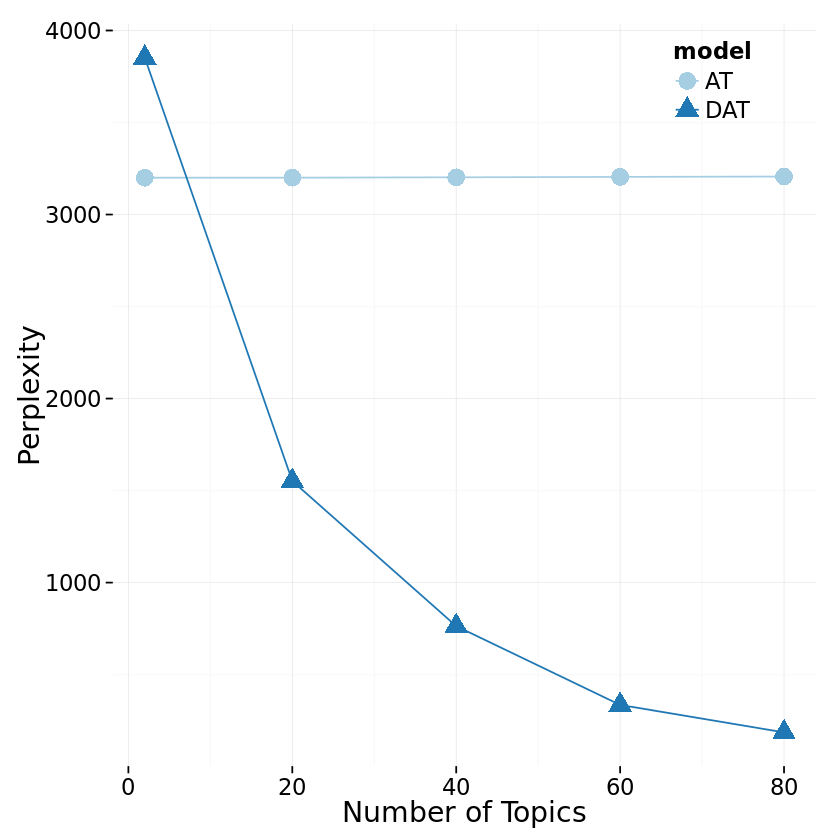
\includegraphics[width=0.7\textwidth]{figures/at_dat_perplexity.png}
\caption{Mean perplexity of DAT and AT with varying numbers of latent topics.}
\label{fig:at_dat_perplexity}
\end{figure}

\subsection{Topic Distribution}\label{at_dat_td}


Similar to Table~\ref{table:ldatopicdistribution}, here we have shown the examples of 6 topics with author information, but here due to space limitation we only show the top 10 most likely words to be generated conditioned on the topic, and 4 top most likely authors to have generated a word conditioned on the topic. The topic-category distribution of the Author-Topic model is shown in Figure~\ref{fig:at_topic_category}. And our interpreting of the topic as well its words distribution can be shown in Table~\ref{table:at_topic_distribution}. 

\begin{figure}[h]
\centering
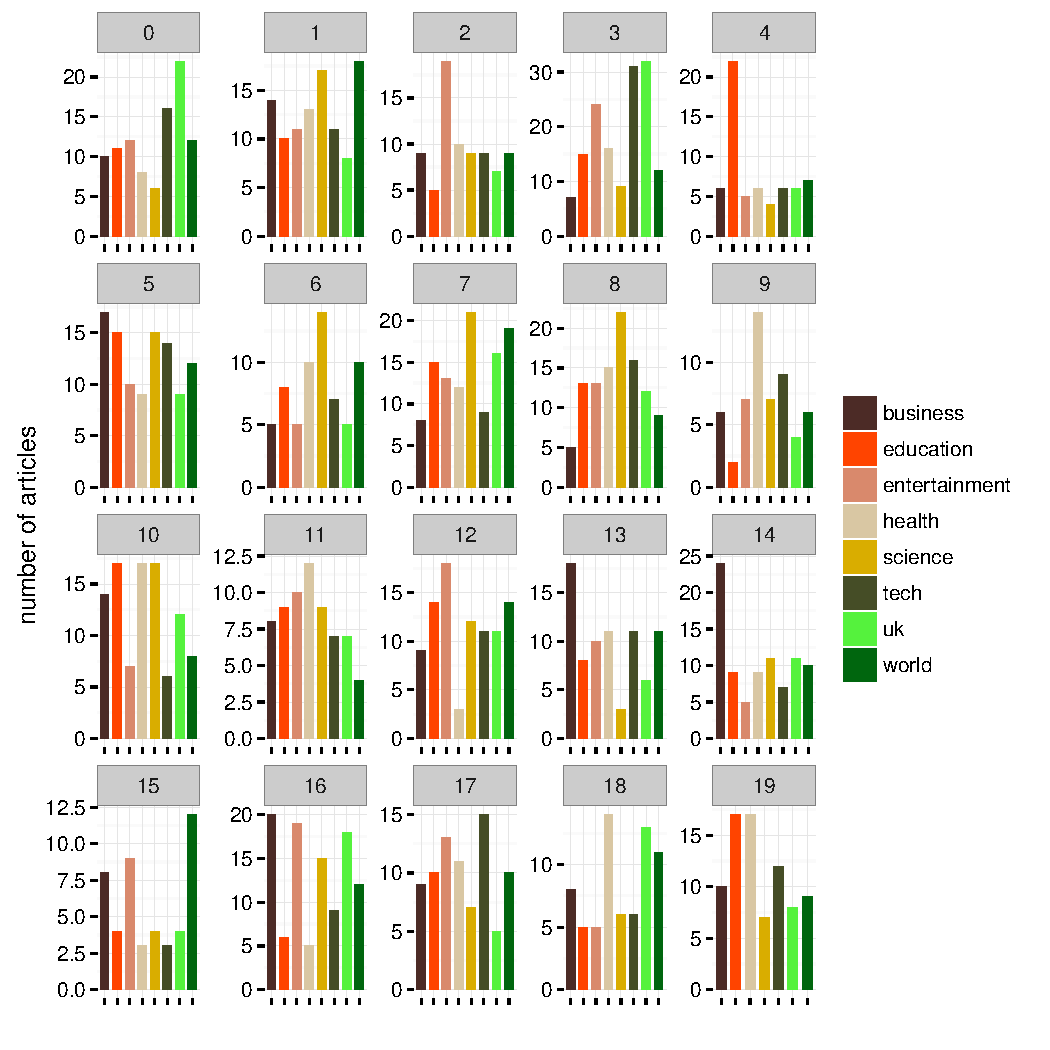
\includegraphics[width=1\textwidth]{figures/at_topic_category.pdf}
\caption{Topic-category distribution of Author-Topic model.}
\label{fig:at_topic_category}
\end{figure}


\begin{table}[h!]
\centering
\begin{tabular}{|c c|} 
\hline
\multicolumn{2}{|c|}{\textbf{Topic 0 : UK}} \\
\hline
 \textbf{WORD} & \textbf{PROB}.  \\ [0.3ex] 
 \hline
 	police  &   0.011306\\
	expect   &  0.007149\\
	attack  &   0.005665\\
	cause  &   0.005397\\
	site  &   0.004464\\
	put   &  0.004408\\
	road   &  0.004307\\
	country  &   0.004144\\
	investigation  &   0.004074\\
	foreign   &  0.003674\\[1ex] 
 \hline
  \textbf{AUTHOR} & \textbf{PROB}.  \\ [0.3ex] 
 \hline
 6  & 0.12136\\
8  &   0.11783\\
5  &   0.11711\\
3  &   0.11258\\
 \hline
\end{tabular}
 \hfill
\begin{tabular}{|c c|} 
\hline
\multicolumn{2}{|c|}{\textbf{Topic 2 : Entertainment}} \\
\hline
 \textbf{WORD} & \textbf{PROB}.  \\ [0.3ex] 
 \hline
 	place  & 0.004633 \\
 	shot   & 0.004466\\
	first  &  0.004243\\
	close  &  0.004184\\
	facebook  &  0.004080\\
	well   &    0.003947\\
	become    &   0.003857\\
	look   &    0.003819\\
	improve   &    0.003753\\
	side    &   0.003694\\[1ex] 
 \hline
  \textbf{AUTHOR} & \textbf{PROB}.  \\ [0.3ex] 
 \hline
 7  & 0.12367\\
4   &  0.11519\\
2  &   0.11368\\
3  &   0.11360\\
 \hline
\end{tabular}
 \hfill
 \begin{tabular}{|c c|} 
\hline
\multicolumn{2}{|c|}{\textbf{Topic 4 : Education}} \\
\hline
 \textbf{WORD} & \textbf{PROB}.  \\ [0.3ex] 
 \hline
 part  & 0.006973 \\
	girl  &  0.005364\\
	man   & 0.005104\\
	read  &  0.004729\\
	school  &  0.004672\\
	appeal   & 0.004640\\
	parent   & 0.004473\\
	reveal  &  0.004416\\
	go   & 0.004294\\
	public  &  0.004241 \\ [1ex] 
 \hline
  \textbf{AUTHOR} & \textbf{PROB}.  \\ [0.3ex] 
 \hline
 0  & 0.12073 \\ 
1   &  0.11673 \\ 
4  &   0.11618 \\ 
7  &   0.112373 \\ 
 \hline
\end{tabular}
\hfill
\\[1cm]
\begin{tabular}{|c c|} 
\hline
\multicolumn{2}{|c|}{\textbf{Topic 14 : Business}} \\
\hline
 \textbf{WORD} & \textbf{PROB}.  \\ [0.3ex] 
 \hline
 many &  0.005329 \\ 
	like  &    0.005039 \\ 
	need   &   0.004944 \\ 
	month  &    0.004247 \\ 
	made  &    0.004159 \\ 
	charge  &    0.004054 \\ 
	make  &    0.003994 \\ 
	price  &    0.003814 \\ 
	case  &    0.003686 \\ 
	union  &    0.003612 \\ [1ex] 
 \hline
  \textbf{AUTHOR} & \textbf{PROB}.  \\ [0.3ex] 
 \hline
 7 &  0.12653 \\
3 &   0.11960 \\
5 &   0.11089 \\
2 &   0.11010  \\
 \hline
 \end{tabular} 
\hfill
 \begin{tabular}{|c c|} 
\hline
\multicolumn{2}{|c|}{\textbf{Topic 15 : World}} \\
\hline
 \textbf{WORD} & \textbf{PROB}.  \\ [0.3ex] 
 \hline
 live  & 0.005703\\ 
	die   &  0.004945\\ 
	ahead  &   0.004934\\ 
	man   &  0.004902\\ 
	govern  &   0.004725\\ 
	tax   &  0.004625\\ 
	author  &   0.004103\\ 
	hope   &  0.004006\\ 
	member  &   0.003923\\ 
	conservative  &   0.003762\\ [1ex] 
 \hline
  \textbf{AUTHOR} & \textbf{PROB}.  \\ [0.3ex] 
 \hline
 3 &   0.11515 \\
4  &    0.11366 \\
5   &   0.11247 \\
0  &    0.11227  \\
 \hline
 \end{tabular} 
\hfill
\begin{tabular}{|c c|} 
\hline
\multicolumn{2}{|c|}{\textbf{Topic 18 : Health}} \\
\hline
 \textbf{WORD} & \textbf{PROB}.  \\ [0.3ex] 
 \hline
 state &  0.006794 \\ 
	announce  &   0.005624 \\ 
	head  &   0.004991 \\ 
	govern &    0.004573 \\ 
	case &    0.004527 \\ 
	health &    0.004502 \\ 
	number &    0.004211 \\ 
	country&    0.004123 \\ 
	shop  &   0.003961 \\ 
	council &  0.003655 \\ [1ex] 
 \hline
  \textbf{AUTHOR} & \textbf{PROB}.  \\ [0.3ex] 
 \hline
 7 &  0.12653 \\
3 &   0.11960 \\
5 &   0.11089 \\
2 &   0.11010  \\
 \hline
 \end{tabular} 
\hfill
\caption{The topic distribution of Author-Topic model}
\label{table:at_topic_distribution}
\end{table}

We can see that the authorship is evenly distributed over the topics which means the authorship information is not very useful in our case since the authors' contribution for each topic can not be differentiated easily. The reason is that our nine authors are virtually set and our expectation that the news in different categories are different has limited the flexibility of the topic assignment of the DAT model. To compare we have selected the BBC news published in the week of May 6th (which is different from the weeks in Section~\ref{sec:ldadat}). We can see that the word distribution for DAT model is more specific and the author distribution is more diverse than AT model.  


\begin{table}[h!]
\centering
\begin{tabular}{|c c|} 
\hline
\multicolumn{2}{|c|}{\textbf{Topic 0 : UK}} \\
\hline
 \textbf{WORD} & \textbf{PROB}.  \\ [0.3ex] 
 \hline
 	party &  0.029783\\
	conserve  &   0.020655\\
	chief  &   0.018636\\
	industry  &   0.018239\\
	parliament  &   0.014519\\
	role  &   0.013771\\
	allow  &   0.012798\\
	leave  &   0.012498\\
	challenge   &  0.012423\\
	secretary   &  0.012295\\[1ex] 
 \hline
  \textbf{AUTHOR} & \textbf{PROB}.  \\ [0.3ex] 
 \hline
 2 &  0.12066\\
1  & 0.11389\\
5  & 0.10803\\
6  & 0.098594\\
 \hline
\end{tabular}
 \hfill
\begin{tabular}{|c c|} 
\hline
\multicolumn{2}{|c|}{\textbf{Topic 4 : World}} \\
\hline
 \textbf{WORD} & \textbf{PROB}.  \\ [0.3ex] 
 \hline
 	police &  0.054837\\
	state &   0.025174\\
	area &   0.022276\\
	party &   0.018467\\
	elect &   0.016934\\
	trade &   0.015518\\
	trump &   0.014928\\
	power &   0.014887\\
	provide &   0.014036\\
	uk &   0.013866\\[1ex] 
 \hline
  \textbf{AUTHOR} & \textbf{PROB}.  \\ [0.3ex] 
 \hline
0 &  0.12009\\
2 &  0.11484\\
1 &  0.11441\\
5  & 0.10904\\
 \hline
\end{tabular}
 \hfill
 \begin{tabular}{|c c|} 
\hline
\multicolumn{2}{|c|}{\textbf{Topic 9 : Education}} \\
\hline
 \textbf{WORD} & \textbf{PROB}.  \\ [0.3ex] 
 \hline
 support &  0.023740\\
	make  &    0.022040\\
	family   &   0.016543\\
	assemble  &   0.015807\\
	school   &   0.015694\\
	children  &    0.015580\\
	site   &   0.015215\\
	injury   &   0.014731\\
	cost   &   0.013979\\
	help   &   0.013598\\ [1ex] 
 \hline
  \textbf{AUTHOR} & \textbf{PROB}.  \\ [0.3ex] 
 \hline
 6 &  0.11991 \\ 
4  &    0.11339\\
2  &    0.11301\\
8  &    0.11194 \\ 
 \hline
\end{tabular}
\hfill
\\[1cm]
\begin{tabular}{|c c|} 
\hline
\multicolumn{2}{|c|}{\textbf{Topic 15 : UK Politics}} \\
\hline
 \textbf{WORD} & \textbf{PROB}.  \\ [0.3ex] 
 \hline
	world &  0.023130\\
	london &   0.019875\\
	south &   0.019585\\
	product &   0.017882\\
	elect &   0.016504\\
	vote &   0.016387\\
	finance &   0.015132\\
	depart &   0.014511\\
	agency &   0.013886\\
	david &   0.012805\\ [1ex] 
 \hline
  \textbf{AUTHOR} & \textbf{PROB}.  \\ [0.3ex] 
 \hline

4 &  0.11802\\
8  &   0.11681\\
1   &  0.11148\\
2   &  0.11089\\
 \hline
 \end{tabular} 
\hfill
 \begin{tabular}{|c c|} 
\hline
\multicolumn{2}{|c|}{\textbf{Topic 16 : Health}} \\
\hline
 \textbf{WORD} & \textbf{PROB}.  \\ [0.3ex] 
 \hline
	health  & 0.020498\\
	change  &  0.020243\\
	company  &  0.019476\\
	road   & 0.017493\\
	care  &  0.01701\\
	woman &   0.014633\\
	import  &  0.014289\\
	england   & 0.014035\\
	hospital  &  0.013980\\
	claim  &  0.013552\\ [1ex] 
 \hline
  \textbf{AUTHOR} & \textbf{PROB}.  \\ [0.3ex] 
 \hline
 3 &  0.11886\\
5  &   0.11264\\
1  &   0.11230\\
8  &   0.10943  \\
 \hline
 \end{tabular} 
\hfill
\begin{tabular}{|c c|} 
\hline
\multicolumn{2}{|c|}{\textbf{Topic 18 : Business}} \\
\hline
 \textbf{WORD} & \textbf{PROB}.  \\ [0.3ex] 
 \hline
 service &  0.029095 \\
	issue &     0.025055 \\
	held   &   0.020426 \\
	help   &   0.020279 \\
	investigation &     0.017410 \\
	event   &   0.016605 \\
	ad   &   0.016459 \\
	former  &    0.016311 \\
	leave   &   0.016091 \\
	prime &     0.014764 \\ [1ex] 
 \hline
  \textbf{AUTHOR} & \textbf{PROB}.  \\ [0.3ex] 
 \hline
5  & 0.11912\\
0   &  0.11677 \\
3  &   0.11633\\
8  &   0.11203  \\
 \hline
 \end{tabular} 
\hfill
\caption{The topic distribution of Dynamic Author-Topic model on May 6th}
\label{table:datat_topic_distribution}
\end{table}


We also see that the words generated for each topic using AT model is also general as LDA model. To answer \textbf{RQ1,3,4}, by comparing with our experimental results in Section \ref{sec:ldadat} definitely DAT works much better than AT model.


\section{Performance Comparison between Dynamic Author-Topic and Topic Tracking models}
In this section we will compare the performance of Topic Tracking model and the Dynamic Author-Topic model. The parameters of TTM model is set as $\alpha = 0.1$, and $\beta = 0.01$. DAT model has the same parameter setup besides that its author number is 9. For both the model the topic numbers are set as 20 for the experiment in Section \ref{dat_ttm_td}.
\subsection{Perplexity}
\begin{figure}[h]
\centering
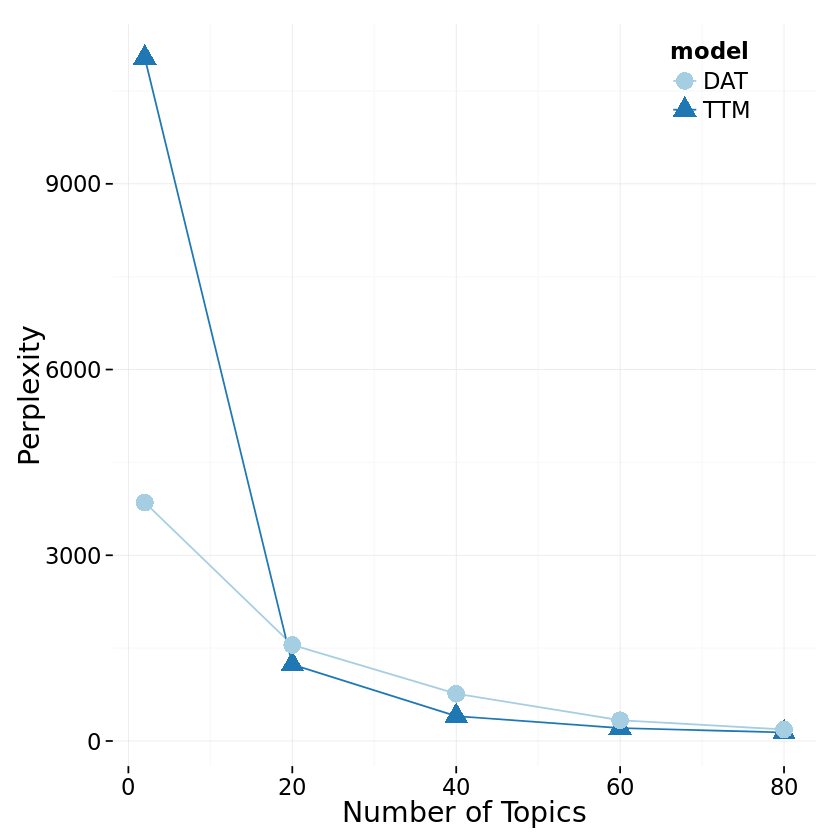
\includegraphics[width=0.7\textwidth]{figures/ttm_data_perplexity.png}
\caption{Mean perplexity of DAT and TTM with varying numbers of latent topics.}
\label{fig:ttm_dat_perplexity}
\end{figure}

The perplexity comparison between LDA and DAT model is shown in Figure~\ref{fig:ttm_dat_perplexity}, to answer \textbf{RQ6}, with small number of topics our DAT model performs better than TTM model, whereas with the increasing number of topics, the performances of the two models become to converge. Therefore with large number of topics the two models have a comparable generalization performance. For \textbf{RQ5} the performance of both models becomes better when the topic number is larger.


\subsection{Topic Distribution}\label{dat_ttm_td}

Again here we try to evaluate the classification performance of the two model in order to answer \textbf{RQ1, 3, 4} using the same methodology as in Section~\ref{ldadat_td}. In this section we will mainly show the experimental results of TTM model which will be compared with the results of DAT model as discussed in Section~\ref{ldadat_td}. We also use the same four weeks' data as those for DAT model in Section~\ref{ldadat_td}, which are the weeks from Jan 1 to Jan 7, from Feb 12 to Feb 19, from Jan Mar 4 to Mar 11, and from May 20 to May 27, so that the comparison of the experimental results of the two models are meaningful. 

\begin{figure*}[!t]
  \centering
    \subfigure[2016.01.01 to 2016.01.07]{
    \label{subfig:11ttmtopiccategory} 
    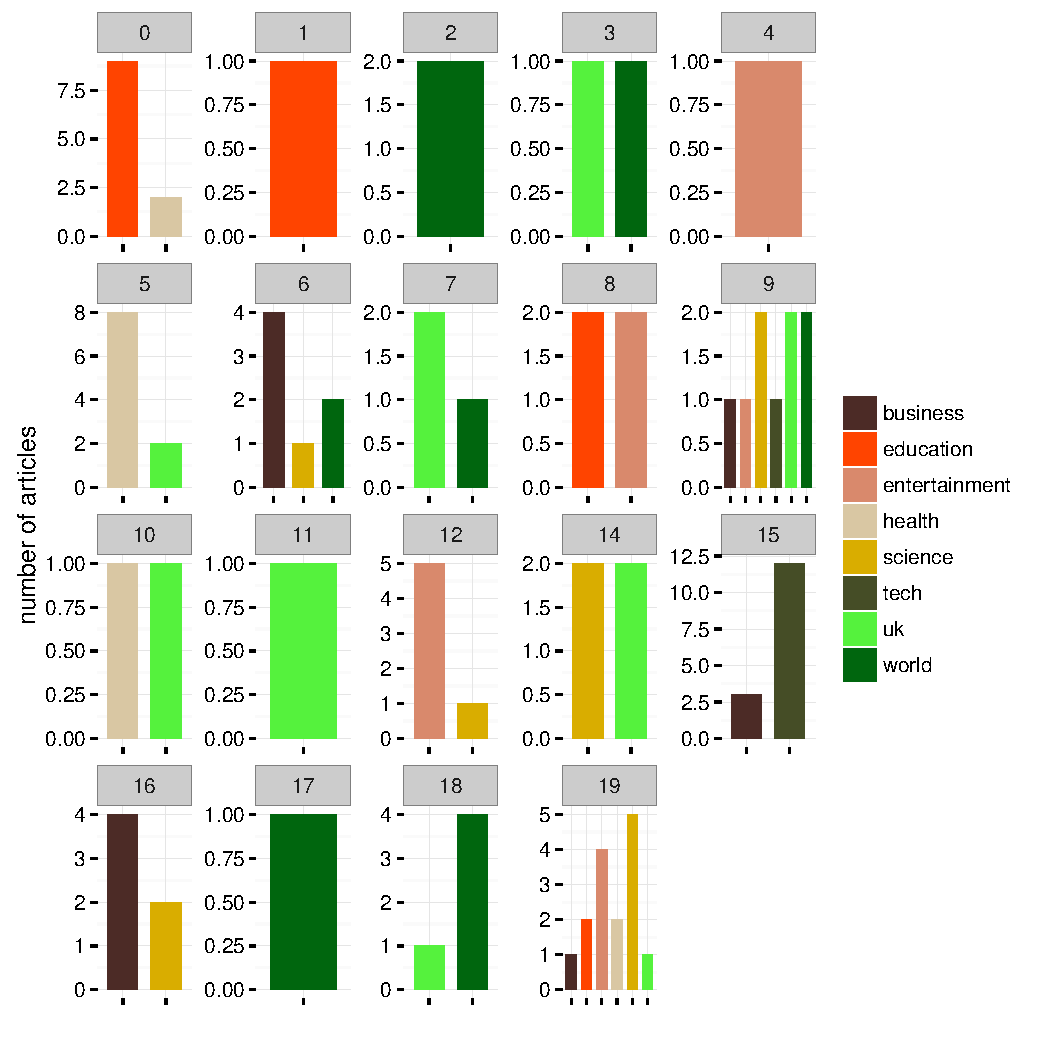
\includegraphics[width=.48\columnwidth]{figures/11ttmcatogery.pdf}}
    \subfigure[2016.02.12 to 2016.02.19]{
    \label{subfig:212ttmtopiccategory} 
    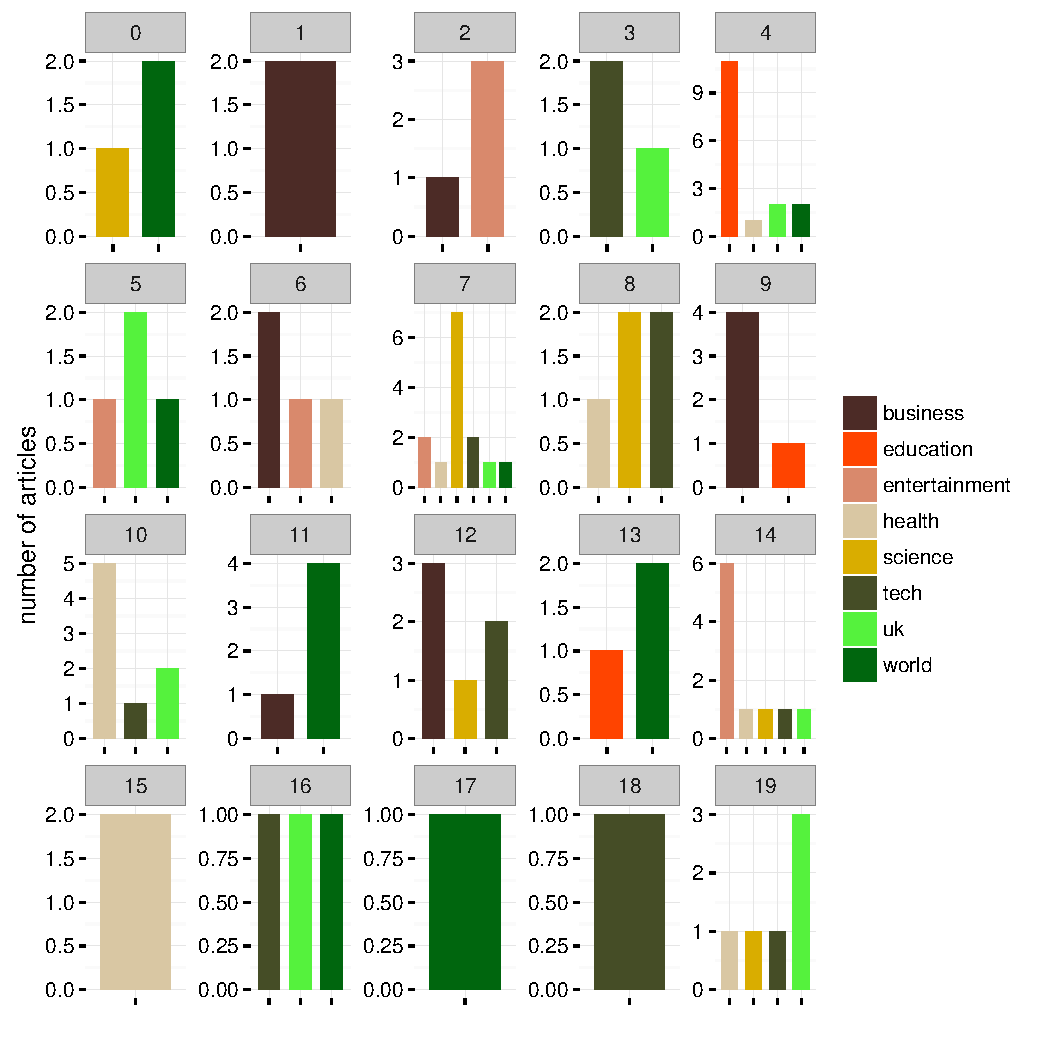
\includegraphics[width=.48\columnwidth]{figures/212ttmcatogery.pdf}}
    \vspace*{-.9\baselineskip}
    \subfigure[2016.03.04 to 2016.03.11]{
    \label{subfig:34ttmtopiccategory} 
    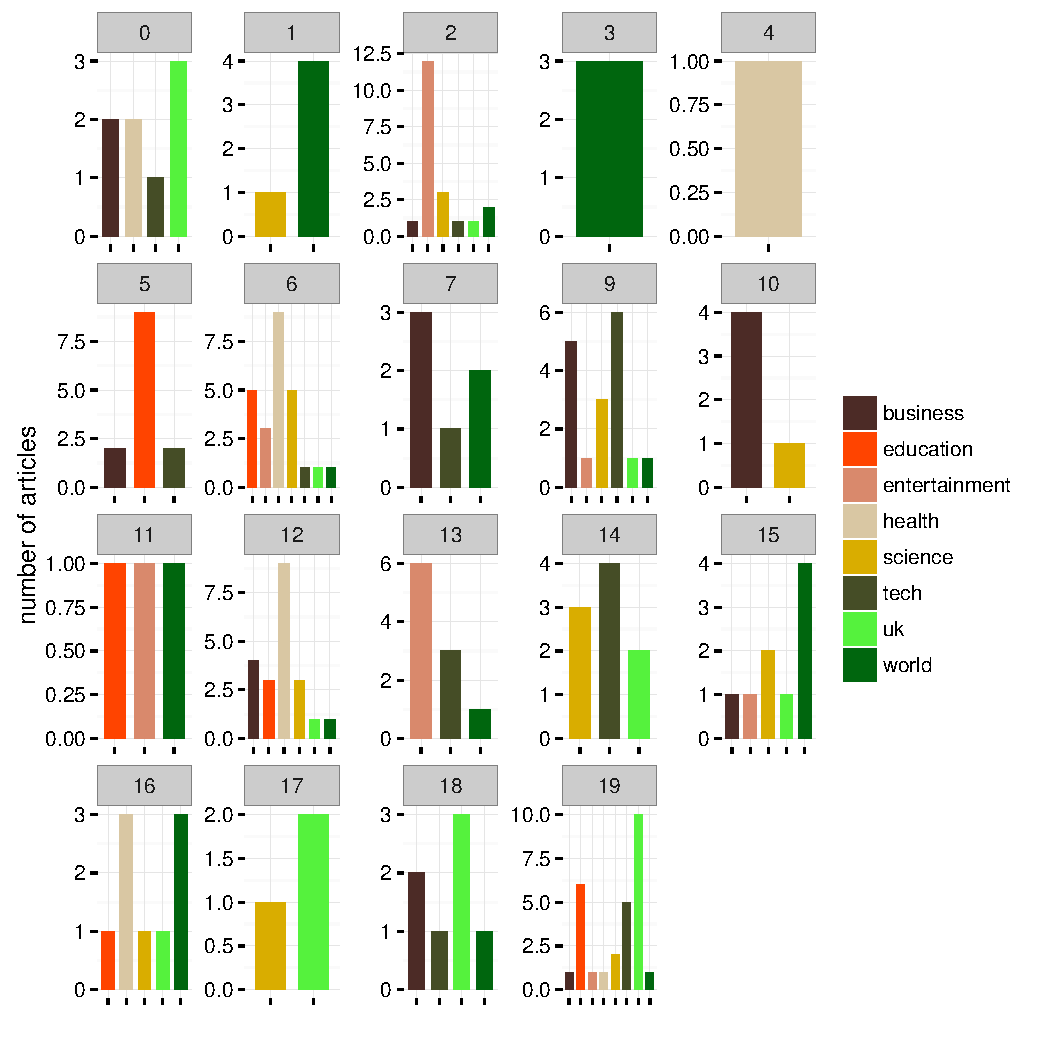
\includegraphics[width=.48\columnwidth]{figures/34ttmcatogery.pdf}}
    \subfigure[2016.05.20 to 2016.05.27]{
    \label{subfig:520ttmtopiccategory} 
    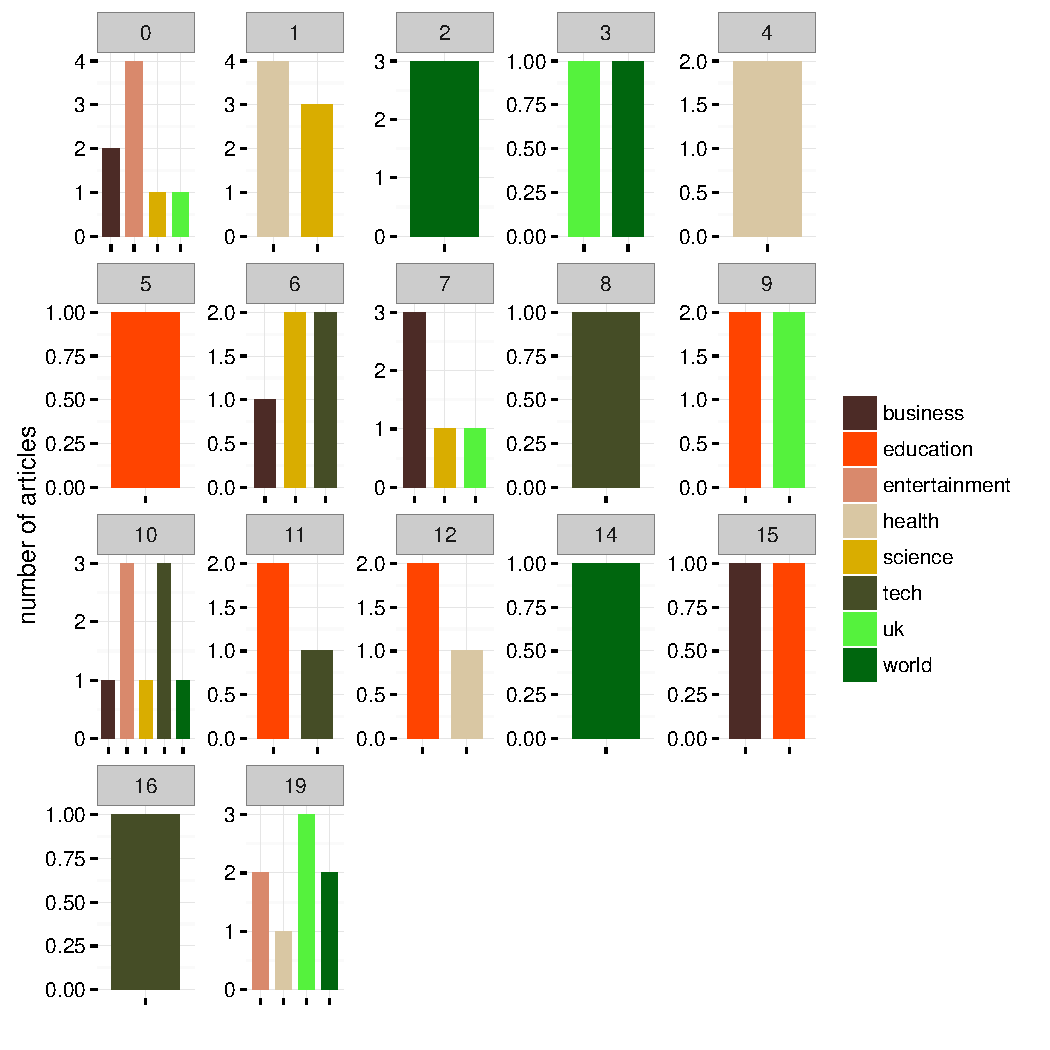
\includegraphics[width=.48\columnwidth]{figures/520ttmcatogery.pdf}}
\caption{\small Topic-category distribution of TTM model for 4 different weeks, which are between 2016.01.01 to 2016.01.07, between 2016.02.12 to 2016.02.19, between 2016.03.04 to 2016.03.11 and between 2016.05.20 to 2016.05.27.}
\label{fig:ttmtopiccategory}
\end{figure*}

In Figure~\ref{fig:ttmtopiccategory} we present the topic-category distribution for TTM model for the four weeks, based on which we will interpret the real meaning underlying these topics so that we can further discover the topic evolution for TTM model. Figure~\ref{fig:ttmtopiccategory} shows that TTM's topics are also neatly and time-related, which is also better than LDA model. Compared to DAT model the topics of TTM are more prominent and topic segmentation are more distinctive.  

Figure \ref{fig:ttm_education_tc}, Figure \ref{fig:ttm_uk_tc} and Figure \ref{fig:ttm_health_tc} here are used to show the evolution of the three topics, \textit{education, UK}, an \textit{health}, which can be respectively compared to the results of DAT model in Figure \ref{fig:dat_education_tc}, Figure~\ref{fig:dat_uk_tc} and Figure \ref{fig:dat_health_tc}.

In Figure~\ref{fig:ttm_education_tc} it shows the topic evolution of \textit{education} for TTM model, compared to the result of DAT in Figure~\ref{fig:dat_education_tc}, we can see the following difference:
\begin{itemize}
    \item In the week of Jan 1st, for TTM model, we see the word of \textit{pupil} because of the news \textit{Every pupil in England will be expected to have memorised their times tables before leaving primary school, under new government plans}~\footnote{http://www.bbc.co.uk/news/education-35216318}, all the other words are general words related to education with no surprise, in contrast to DAT model where we see the words like \textit{islam} due to some specific news event.
    \item In the week of Feb 12th, for TTM model it looks like it has confused between the topic of \textit{education} and \textit{UK}. Since words like \textit{party, Scotland} are obviously UK news related.
    \item In the week of Mar 4th, for TTM model, we see the word \textit{pay} due to the news that \textit{School results don't justify academy trust pay}~\footnote{http://www.bbc.co.uk/news/education-35775458}, and \textit{force} due to the discussion that \textit{Are cadets a force for good in schools}~\footnote{http://www.bbc.co.uk/news/education-35780633}, here we see that TTM and DAT have discovered hot news in this week.
    \item In the week of May 20th, we can see the topics discovered by TTM is quite different from DAT model. The news of \textit{A petition against government plans to freeze the salary threshold at which graduates must start paying back their student loans has topped 100,000 signatures}~\footnote{http://www.bbc.co.uk/news/education-36420790} and \textit{Scotland lags behind on poorer students}~\footnote{http://www.bbc.co.uk/news/education-36392685} are successfully discovered in the topic, while for DAT the topics is more focused on the news event like stopping publishing primary school students' score and some related to EU referendum.
\end{itemize}

In Figure~\ref{fig:ttm_uk_tc} it shows the topic evolution of \textit{UK} for TTM model, compared to the result of DAT in Figure~\ref{fig:dat_uk_tc}, we can see the following difference:
\begin{itemize}
    \item In the week of Jan 1st, for TTM model, we see the words are relative general compared to that of DAT model, and the news related to \textit{murder} is ignored by TTM model which could be hot news for that week. 
    \item In the week of Feb 12th, TTM model performs very well for discovering the Syria related UK news, such as \textit{UK's Syria air strikes killed or injured 'seven IS fighters'}~\footnote{http://www.bbc.co.uk/news/uk-35607446} in which \textit{missile} is mentinoed a lot of times. However we see the word \textit{Korea} due to the news about \textit{new North Korea sanctions} because of its missile launch, which is actually a \textit{world} news. Therefore TTM is confounding the UK news and world news because that \textit{missile} and \textit{Syria}, \textit{Korea} all co-occurred.
    \item In the week of Mar 4th, the TTM model also discovered the London mayor election, which is also found by DAT model. 
    \item In the week of May 20th, all the top five words of topic \textit{UK} for TTM model is election related which is exactly the hot news in these days. DAT also discovered the election but its word distribution is more diverse. In this case for TTM model its word distribution can describe the topic's content very well whereas DAT outperforms in terms  the discovery of specific and diverse hot news.
    \end{itemize}
    
In Figure~\ref{fig:ttm_health_tc} it shows the topic evolution of \textit{health} for TTM model, compared to the result of DAT in Figure~\ref{fig:dat_health_tc}, we can see the following difference:
\begin{itemize}
    \item In the week of Jan 1st, for TTM model, we see the words are general compared to that of DAT model, all the words are apparently health related.
    \item In the week of Feb 12th, TTM outperforms DAT for pinpointing the news about Zika virus~\footnote{http://www.bbc.co.uk/news/health-35597465}~\footnote{http://www.bbc.co.uk/news/health-35552340}. The word black is there is because of the news \textit{Mental health care for black men in England criticised}~\footnote{http://www.bbc.co.uk/news/uk-england-35606171}.
    \item In the week of Mar 4th, the word distribution for TTM model is similar to that of DAT model, the word \textit{Scotland} appears because of the discussion in a few news about the rise of the pay for health workers in Scotland.
    \item In the week of May 20th, it looks like TTM has confused about the topic of \textit{health} and \textit{UK politics}. DAT outperforms TTM for this week since DAT's words are more health related.
    \end{itemize}

\begin{figure}[h]
\centering
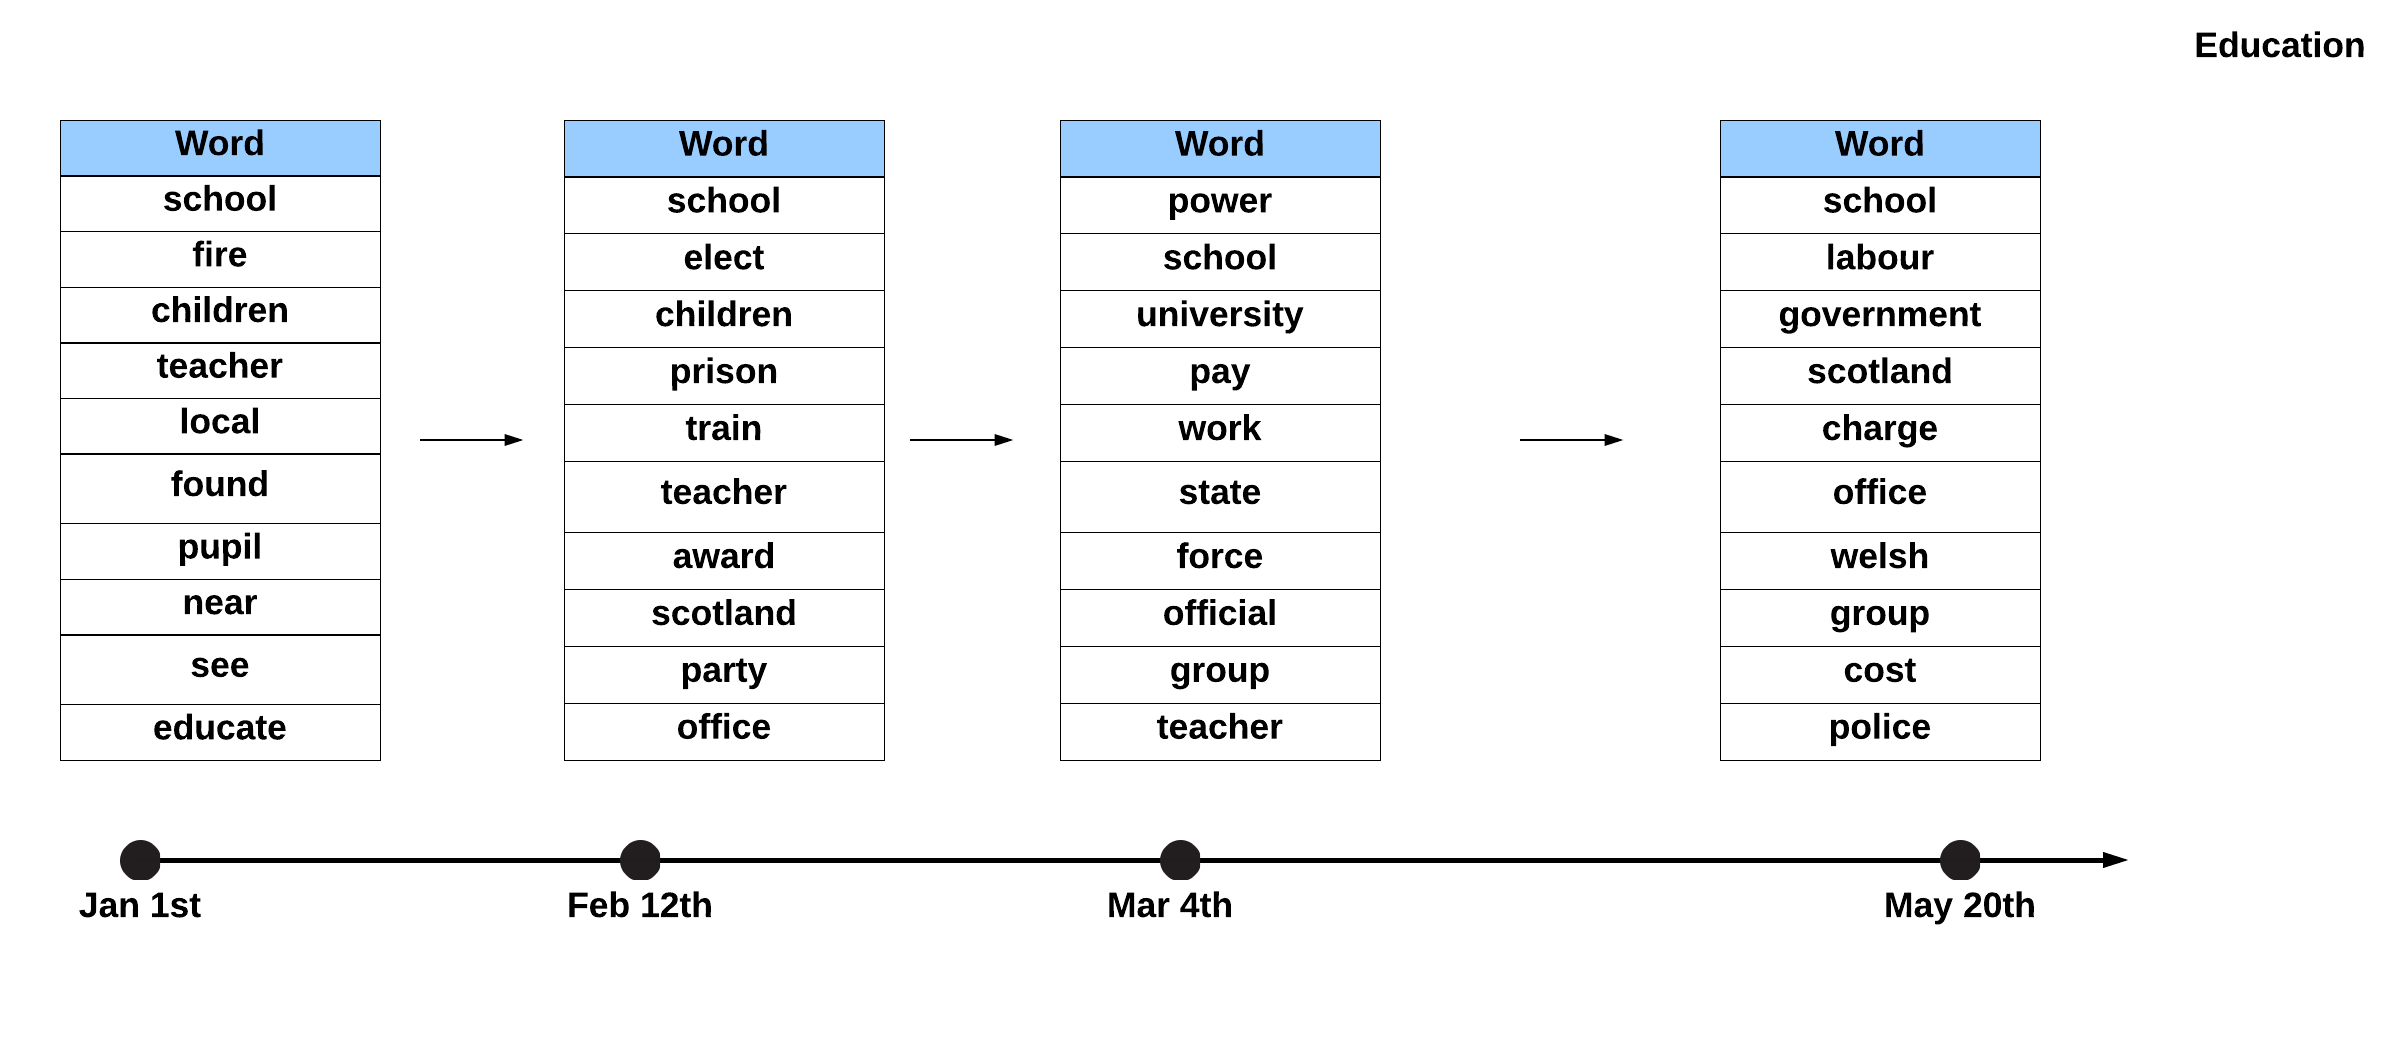
\includegraphics[width=1\textwidth]{figures/ttm_education_tc.png}
\caption{Topic evolution of TTM model: use Education as an example}
\label{fig:ttm_education_tc}
\end{figure}
\begin{figure}[h]
\centering
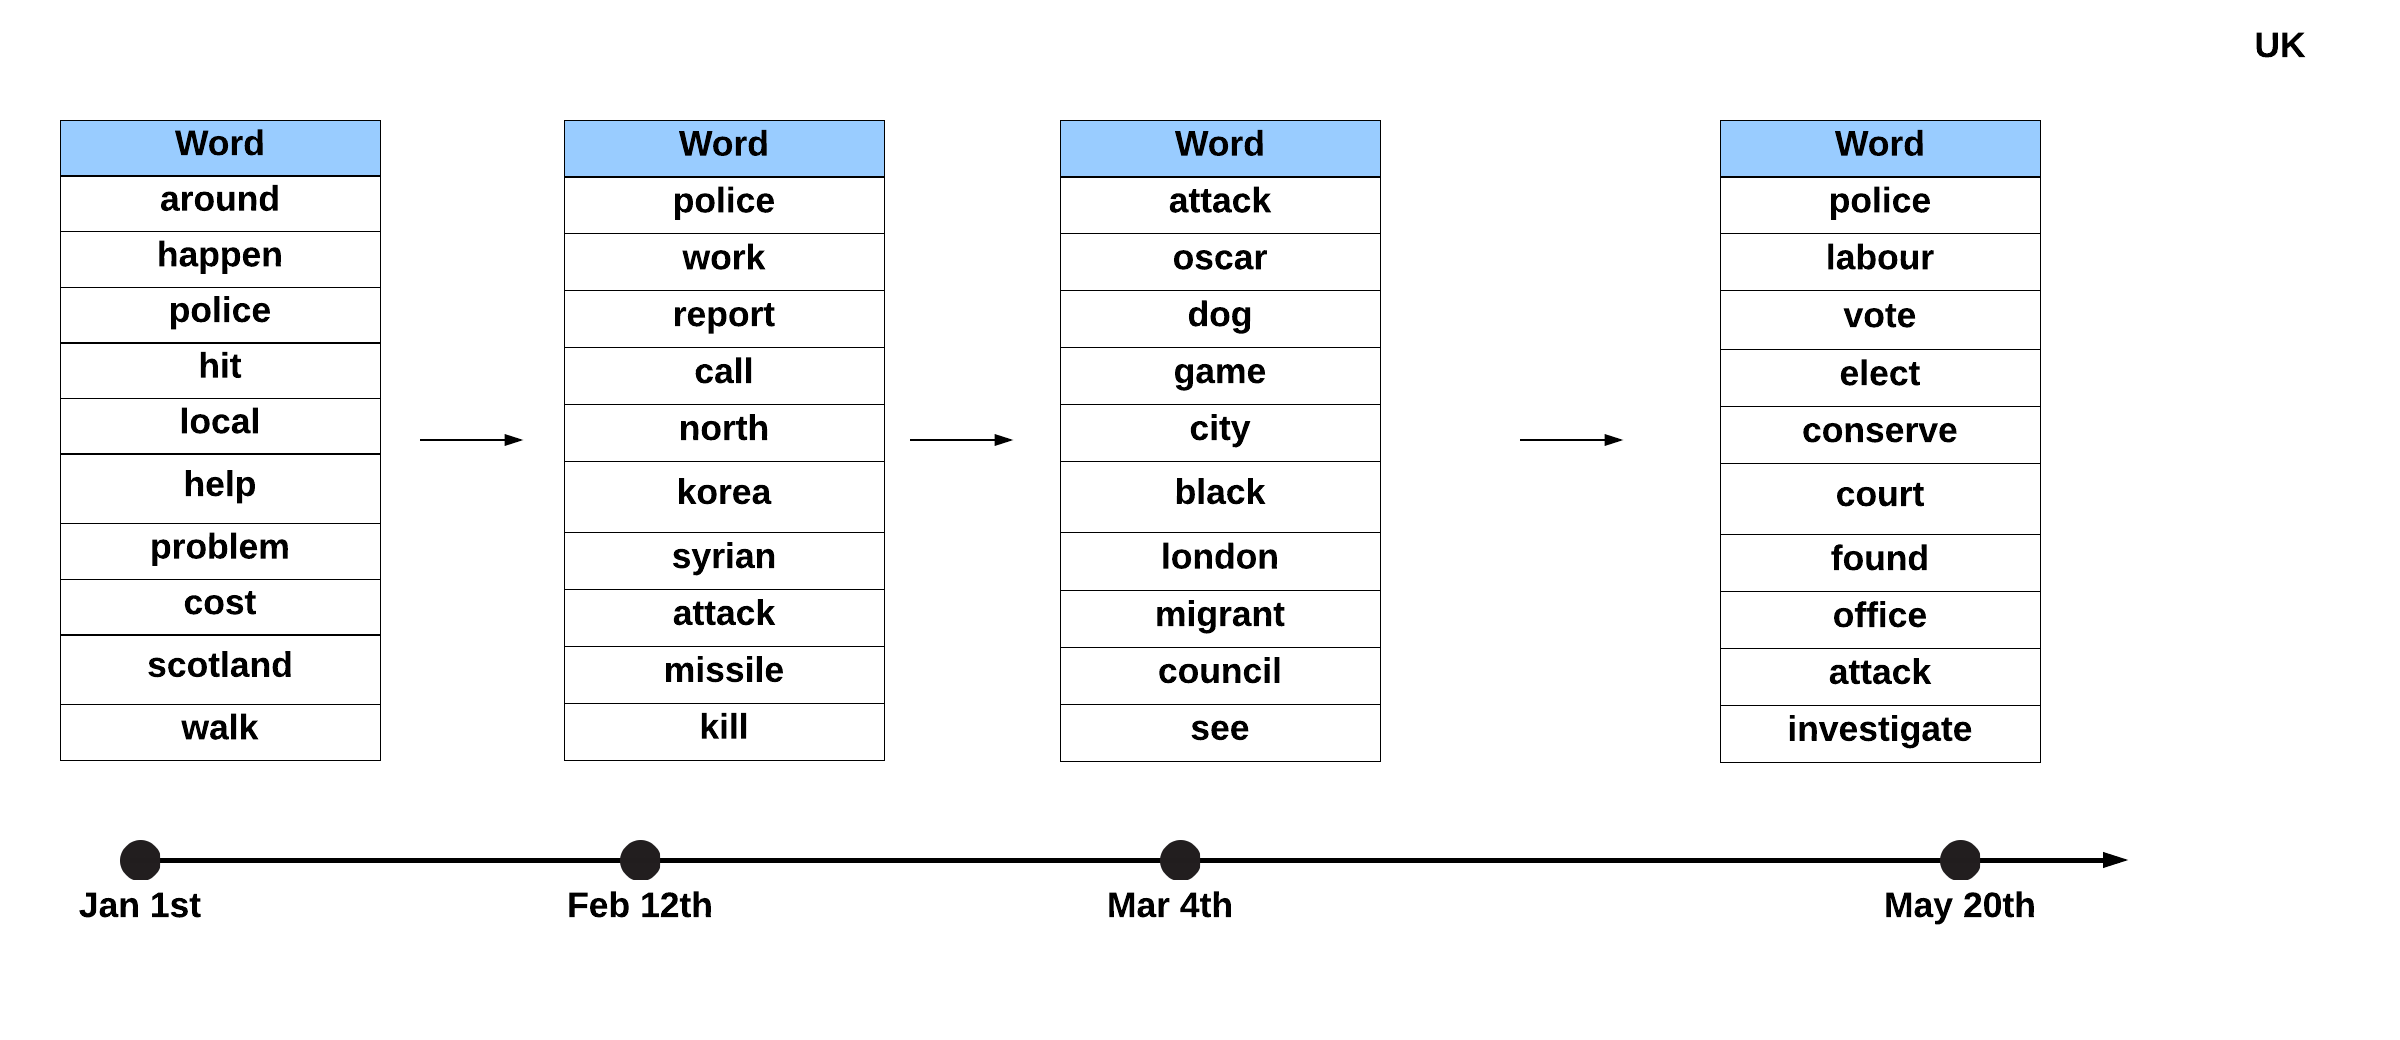
\includegraphics[width=1\textwidth]{figures/ttm_uk_tc.png}
\caption{Topic evolution of TTM model: use UK as an example}
\label{fig:ttm_uk_tc}
\end{figure}
\begin{figure}[h]
\centering
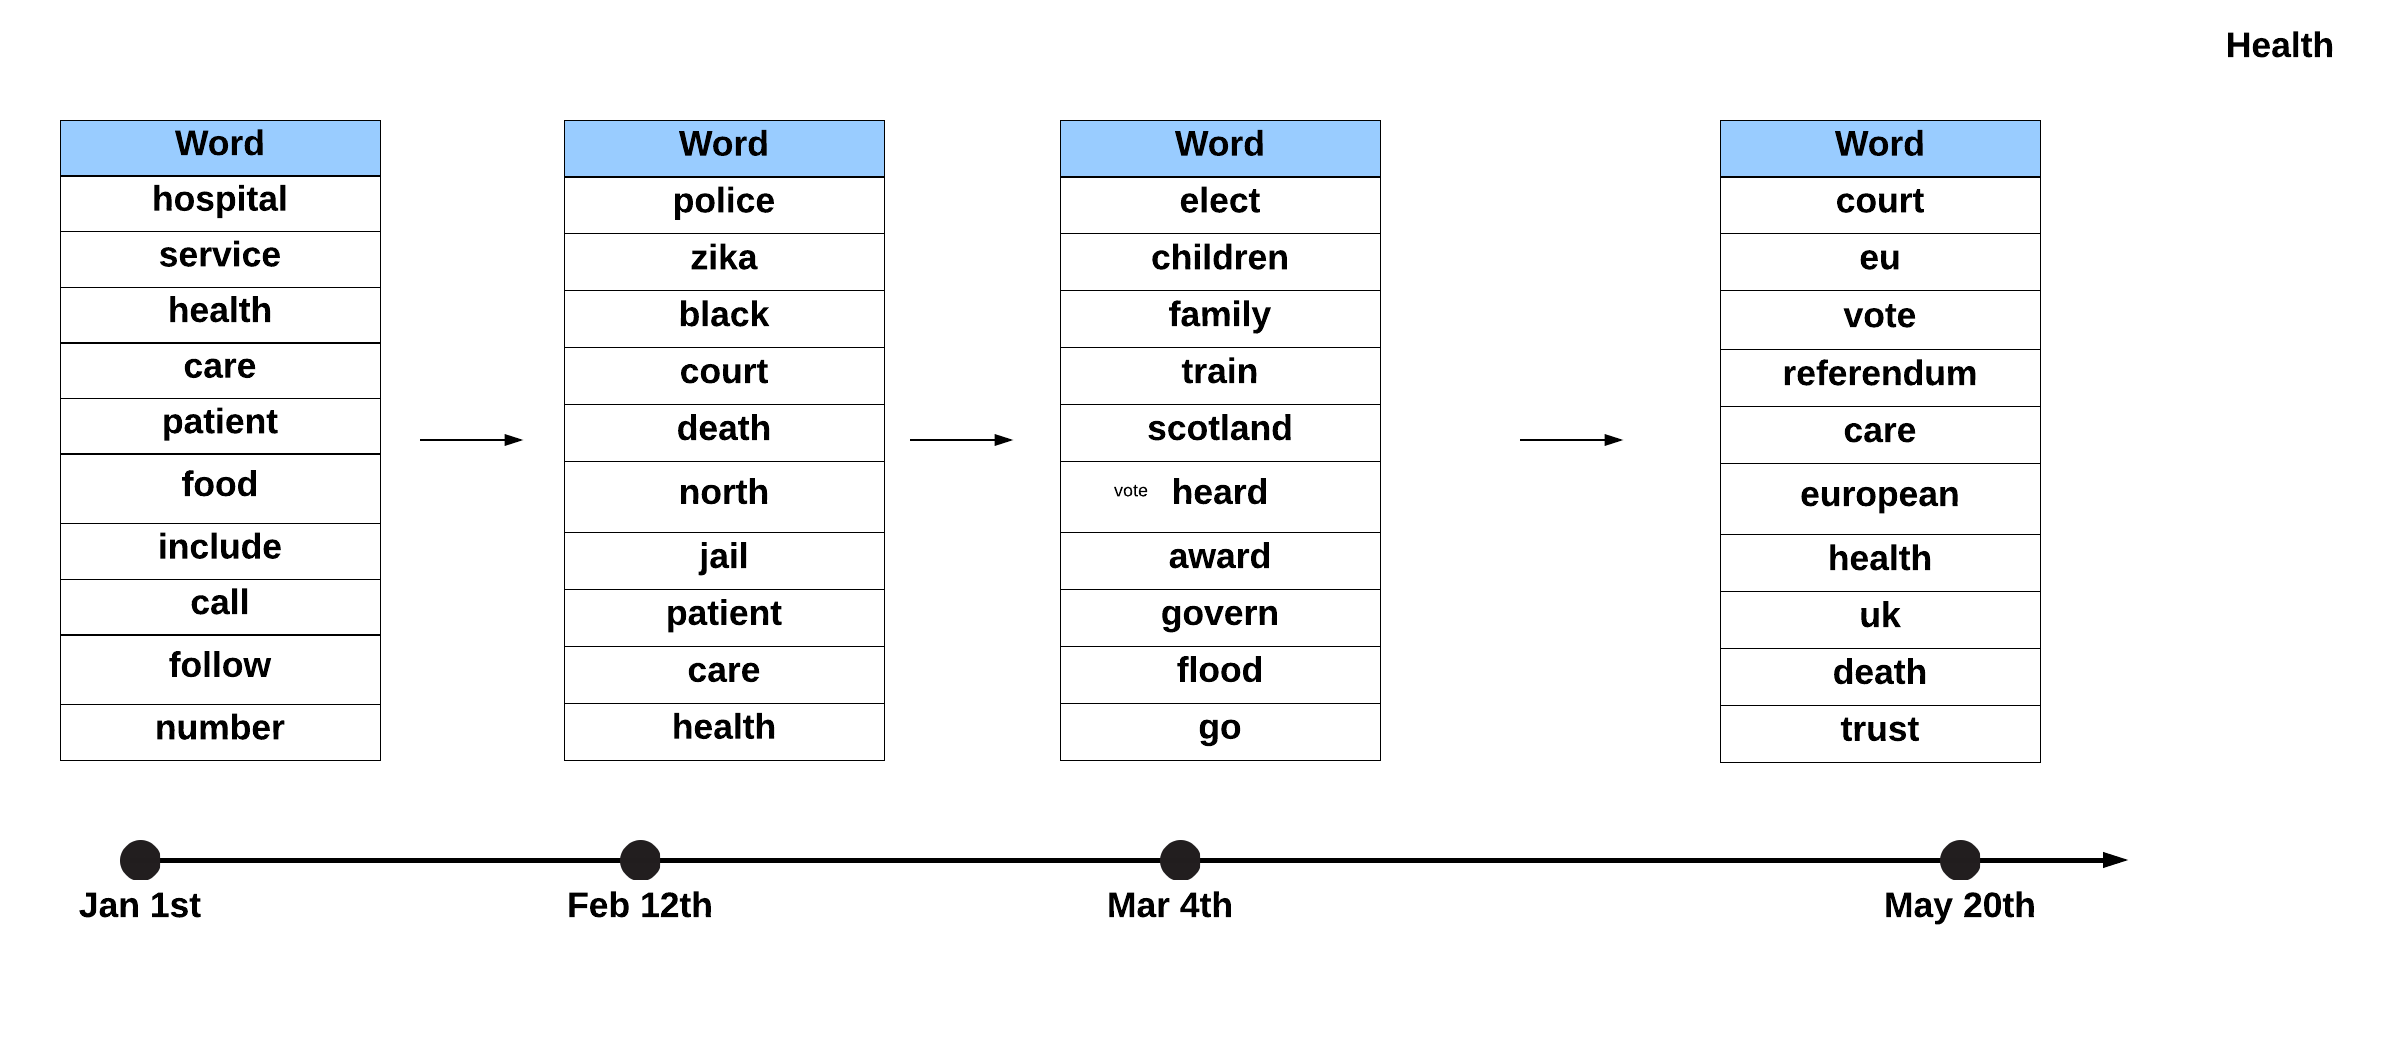
\includegraphics[width=1\textwidth]{figures/ttm_health_tc.png}
\caption{Topic evolution of TTM model: use Health as an example}
\label{fig:ttm_health_tc}
\end{figure}

In conclusion, to answer \textbf{RQ1}, TTM performs better than DAT in terms of segment topics, the topic-category distribution of TTM model is more prominent and distinctive than DAT model which means it is easy to tell the correspondence between category $c$ and topic $z$, however TTM has the drawback that its word description for a topic is always general and confounding on some news events with co-occurrence word patterns, its topic evolution is not as clear as DAT model. DAT model outperforms TTM model since (a) it is able to discover diverse and specific news event and (b) it is topic evolution successfully follow the rise and fall of the topic trending which is beneficial and more accurate to classify specific hot news. 



\section{Comprehensive Comparison}
Based on our experiments in Section 5.1 to 5.3, we can answer our research questions as follows,
\begin{description}
	\item On the basis of classification performance:
	\begin{description}
	\item[\textbf{RQ1}:] The performance of topic extraction is observed with the following order: $\text{DAT} \geq \text{TTM} > \text{LDA} > \text{AT}$. Both DAT and TTM are able to discover time-narrowed topics but the ones extracted by DAT is more diverse and is able to track the news event trends. AT is inferior to LDA our experiment because of the low number of authors, since we only use virtual author here so the authorship is somewhat randomly assigned which limits the predictive power of the AT model. DAT overcomes this drawback because its parameters are adaptive to the time and content of the news documents. 
	\item[\textbf{RQ3}:] The topic evolution of DAT model is better than TTM model as discussed in Section 5.3.
	\item[\textbf{RQ4}:] The order of the performances of the four models is  
	$\text{DAT} > \text{TTM} > \text{AT} = \text{LDA}$. Since AT and LDA models are both static so it is easily to confuse about the news events spreading through the time. The authorship information of DAT helps it to discover more specific and diverse hot news topic thanks to the knowledge which provides a better prior for the news document. 
	\item[\textbf{RQ5}:] Yes, with the increasing number of topics its performance is getting better.
	\end{description}
	\item On the basis of the generative model:
	\begin{description}
	\item[\textbf{RQ6}:] For a small number of topics, the performance order is	$\text{LDA} > \text{AT} > \text{DAT} > \text{TTM}$. While with the increasing number of topics DAT's performance becomes better and the order should be $\text{DAT} = \text{TTM} > \text{LDA} > \text{AT}$.
	\end{description}
\end{description}


\section{Performance with Different Time Slices}


% This just dumps some pseudolatin in so you can see some text in place.
\subsection{Topic Distribution}
In this part in order to compare to the results in Figure~\ref{fig:dat_health_tc},~\ref{fig:dat_uk_tc} and~\ref{fig:dat_education_tc}, we will show the topic evolution for topic \textit{health, education} and \textit{UK}. The topic number here is set as 20. 

When news dependency term is two week, namely half a month, we show the topic evolution of topic \textit{health} in Table~\ref{dat_2_health_evoluation}.

The topic evolution of topic \textit{UK} is in Table~\ref{dat_2_uk_evoluation}. 

The topic evolution of topic \textit{Education} is in Table~\ref{dat_2_educatoin_evoluation}.

When news dependency term is four weeks, namely a month, we show the topic evolution of topic \textit{health} in Table~\ref{dat_4_health_evoluation}.

The topic evolution of topic \textit{UK} is in Table~\ref{dat_4_uk_evoluation}. 

The topic evolution of topic \textit{Education} is in Table~\ref{dat_4_educatoin_evoluation}.

It can be obviously seen that with the increasing of the length of time dependency, the words to describe the topic becomes more general and the the model starts to confound the news event happening in one time period.

In this chapter the experimental results are shown in different rules as will as the performance comparison of other three baselines. In the next chapter we will give a conclusion of the thesis.

\begin{table}
\caption{Topic distribution evolution for topic Health (2 weeks as a time unit)}
\centering
\begin{tikzpicture}
\node (table) [inner sep=0pt] {
\begin{tabular}{c}
  {Jan 1 - Jan 14} \\
  \hline
  yearold\\
	record \\
	health  \\
	current  \\
	leave  \\
	manage \\
	case \\
	member \\
	system  \\
	damage \\
\end{tabular}  
};
\draw [rounded corners=.5em] (table.north west) rectangle (table.south east);
\end{tikzpicture}
\begin{tikzpicture}
\node (table) [inner sep=0pt] {
\begin{tabular}{c}
{Feb 12 - Feb 26} \\
  \hline
 home  \\
	offer  \\
	involve \\
	help   \\
	across   \\
	health   \\
	service  \\
	include   \\
	public   \\
	statement \\
\end{tabular}
};
\draw [rounded corners=.5em] (table.north west) rectangle (table.south east);
\end{tikzpicture}
\begin{tikzpicture}
\node (table) [inner sep=0pt] {
\begin{tabular}{c}
{Mar 11 - Mar 25} \\
  \hline
 world   \\
	die   \\
	risk  \\
	health   \\
	young   \\
	minister  \\
	investigation   \\
	develop   \\
	programm   \\
	complete   \\
	
\end{tabular}
};
\draw [rounded corners=.5em] (table.north west) rectangle (table.south east);
\end{tikzpicture}
\begin{tikzpicture}
\node (table) [inner sep=0pt] {
\begin{tabular}{c}
{May 5 - May 20} \\
  \hline
health  \\
	road   \\
	student  \\
	minister  \\
	cause  \\
	accord   \\
	incident  \\
	see   \\
	remain  \\
	hospital \\
\end{tabular}
};
\draw [rounded corners=.5em] (table.north west) rectangle (table.south east);
\end{tikzpicture}
\label{dat_2_health_evoluation}
\end{table}

\begin{table}
\caption{Topic distribution evolution for topic UK (2 weeks as a time unit)}
\centering
\begin{tikzpicture}
\node (table) [inner sep=0pt] {
\begin{tabular}{c}
  {Jan 1 - Jan 14} \\
  \hline
  want  \\
	next  \\
	west  \\
	record  \\
	age   \\
	reside  \\
	uk   \\
	rate  \\
	govern  \\
	spokesman   \\

\end{tabular}  
};
\draw [rounded corners=.5em] (table.north west) rectangle (table.south east);
\end{tikzpicture}
\begin{tikzpicture}
\node (table) [inner sep=0pt] {
\begin{tabular}{c}
{Feb 12 - Feb 26} \\
  \hline
 work  \\
	eu  \\
	britain  \\
	recent  \\
	death  \\
	campaign  \\
	differ  \\
	share  \\
	china \\
	syria  \\
\end{tabular}
};
\draw [rounded corners=.5em] (table.north west) rectangle (table.south east);
\end{tikzpicture}
\begin{tikzpicture}
\node (table) [inner sep=0pt] {
\begin{tabular}{c}
{Mar 11 - Mar 25} \\
  \hline
 world   \\
	die   \\
	risk  \\
	health   \\
	young   \\
	minister  \\
	investigation   \\
	develop   \\
	programm   \\
	complete   \\
	
\end{tabular}
};
\draw [rounded corners=.5em] (table.north west) rectangle (table.south east);
\end{tikzpicture}
\begin{tikzpicture}
\node (table) [inner sep=0pt] {
\begin{tabular}{c}
{May 5 - May 20} \\
  \hline
office   \\
	import  \\
	appear \\
	uk  \\
	referendum   \\
	elect  \\
	leave   \\
	ad   \\
	independent   \\
	economy \\
\end{tabular}
};
\draw [rounded corners=.5em] (table.north west) rectangle (table.south east);
\end{tikzpicture}
\label{dat_2_uk_evoluation}
\end{table}

\begin{table}
\caption{Topic distribution evolution for topic Education (2 weeks as a time unit)}
\centering
\begin{tikzpicture}
\node (table) [inner sep=0pt] {
\begin{tabular}{c}
  {Jan 1 - Jan 14} \\
  \hline
  take   \\
	man   \\
	rise  \\
	train  \\
	result \\
	london   \\
	become  \\
	group  \\
	name   \\
	appeal  \\

\end{tabular}  
};
\draw [rounded corners=.5em] (table.north west) rectangle (table.south east);
\end{tikzpicture}
\begin{tikzpicture}
\node (table) [inner sep=0pt] {
\begin{tabular}{c}
{Feb 12 - Feb 26} \\
  \hline
 follow   \\
	family  \\
	call   \\
	school  \\
	fund   \\
	first   \\
	lot   \\
	need  \\
	british  \\
	small  \\
\end{tabular}
};
\draw [rounded corners=.5em] (table.north west) rectangle (table.south east);
\end{tikzpicture}
\begin{tikzpicture}
\node (table) [inner sep=0pt] {
\begin{tabular}{c}
{Mar 11 - Mar 25} \\
  \hline
 back  \\
	like   \\
	school \\
	show  \\
	life \\
	women  \\
	make  \\
	referendum  \\
	polite  \\
	move  \\

\end{tabular}
};
\draw [rounded corners=.5em] (table.north west) rectangle (table.south east);
\end{tikzpicture}
\begin{tikzpicture}
\node (table) [inner sep=0pt] {
\begin{tabular}{c}
{May 5 - May 20} \\
  \hline
london   \\
	concern   \\
	gener  \\
	describe \\
	taken\\
	try  \\
	second   \\
	whether \\
	head   \\
	study   \\
\end{tabular}
};
\draw [rounded corners=.5em] (table.north west) rectangle (table.south east);
\end{tikzpicture}
\label{dat_2_educatoin_evoluation}
\end{table}

\begin{table}
\caption{Topic distribution evolution for topic Health (4 weeks as a time unit)}
\centering
\begin{tikzpicture}
\node (table) [inner sep=0pt] {
\begin{tabular}{c}
  {Jan} \\
  \hline
  care  \\
	team  \\
	nhs   \\
	gener  \\
	public  \\
	price   \\
	life   \\
chang e  \\
	get \\
	decide \\
\end{tabular}  
};
\draw [rounded corners=.5em] (table.north west) rectangle (table.south east);
\end{tikzpicture}
\begin{tikzpicture}
\node (table) [inner sep=0pt] {
\begin{tabular}{c}
{Feb} \\
  \hline
 health  \\
	leave  \\
	action  \\
	set   \\
	follow  \\
	know  \\
	think \\
	death  \\
	road  \\
	must  \\
\end{tabular}
};
\draw [rounded corners=.5em] (table.north west) rectangle (table.south east);
\end{tikzpicture}
\begin{tikzpicture}
\node (table) [inner sep=0pt] {
\begin{tabular}{c}
{Mar} \\
  \hline
 nation   \\
	want  \\
	help  \\
	children  \\
	call   \\
	result   \\
	service   \\
	reason   \\
	air   \\
	public   \\
	
\end{tabular}
};
\draw [rounded corners=.5em] (table.north west) rectangle (table.south east);
\end{tikzpicture}
\begin{tikzpicture}
\node (table) [inner sep=0pt] {
\begin{tabular}{c}
{May} \\
  \hline
	health   \\
	woman   \\
	govern   \\
	form   \\
	victim   \\
	home  \\
	know  \\
	even   \\
	good   \\
	proposal  \\
	
\end{tabular}
};
\draw [rounded corners=.5em] (table.north west) rectangle (table.south east);
\end{tikzpicture}
\label{dat_4_health_evoluation}
\end{table}

\begin{table}
\caption{Topic distribution evolution for topic UK (4 weeks as a time unit)}
\centering
\begin{tikzpicture}
\node (table) [inner sep=0pt] {
\begin{tabular}{c}
  {Jan} \\
  \hline
  police  \\
	office   \\
	staff  \\
	near  \\
	response \\
	rise  \\
	service   \\
	travel   \\
	decide   \\
	eu\\

\end{tabular}  
};
\draw [rounded corners=.5em] (table.north west) rectangle (table.south east);
\end{tikzpicture}
\begin{tikzpicture}
\node (table) [inner sep=0pt] {
\begin{tabular}{c}
{Feb} \\
  \hline
north   \\
	member   \\
	took   \\
	change  \\
	victim  \\
	inform  \\
	war   \\
	level  \\
	differ  \\
	men \\
\end{tabular}
};
\draw [rounded corners=.5em] (table.north west) rectangle (table.south east);
\end{tikzpicture}
\begin{tikzpicture}
\node (table) [inner sep=0pt] {
\begin{tabular}{c}
{Mar} \\
  \hline
 bbc   \\
	want \\
	claim  \\
	human   \\
	office  \\
	challenge \\
	british  \\
	campaign  \\
	admit   \\
	street  \\
	
\end{tabular}
};
\draw [rounded corners=.5em] (table.north west) rectangle (table.south east);
\end{tikzpicture}
\begin{tikzpicture}
\node (table) [inner sep=0pt] {
\begin{tabular}{c}
{May} \\
  \hline
tax \\
	call   \\
	north   \\
	media  \\
	case  \\
	follow  \\
	attack  \\
	minister  \\
	support \\
	police  \\
\end{tabular}
};
\draw [rounded corners=.5em] (table.north west) rectangle (table.south east);
\end{tikzpicture}
\label{dat_4_uk_evoluation}
\end{table}

\begin{table}
\caption{Topic distribution evolution for topic Education (4 weeks as a time unit)}
\centering
\begin{tikzpicture}
\node (table) [inner sep=0pt] {
\begin{tabular}{c}
  {Jan} \\
  \hline
 build  \\
	work  \\
	trust  \\
	carry  \\
	school   \\
	mp  \\
	make  \\
	still  \\
	girl  \\
	many  \\

\end{tabular}  
};
\draw [rounded corners=.5em] (table.north west) rectangle (table.south east);
\end{tikzpicture}
\begin{tikzpicture}
\node (table) [inner sep=0pt] {
\begin{tabular}{c}
{Feb} \\
  \hline
work  \\
	group   \\
	move  \\
	much \\
	part  \\
	cause  \\

	children  \\
	early  \\
	end  \\
	given  \\
\end{tabular}
};
\draw [rounded corners=.5em] (table.north west) rectangle (table.south east);
\end{tikzpicture}
\begin{tikzpicture}
\node (table) [inner sep=0pt] {
\begin{tabular}{c}
{Mar } \\
  \hline
secure  \\
	next  \\
	look   \\
	communicate  \\
	school   \\
	rate   \\
	group   \\
	country  \\
	price   \\
	need  \\


\end{tabular}
};
\draw [rounded corners=.5em] (table.north west) rectangle (table.south east);
\end{tikzpicture}
\begin{tikzpicture}
\node (table) [inner sep=0pt] {
\begin{tabular}{c}
{May} \\
  \hline
since  \\
	could   \\
	govern  \\
	claim   \\
	launch   \\
	school   \\
	turn   \\
	scottish   \\
	social   \\
	universe  \\
	\end{tabular}
};
\draw [rounded corners=.5em] (table.north west) rectangle (table.south east);
\end{tikzpicture}
\label{dat_4_educatoin_evoluation}
\end{table}
\chapter{Conclusions}
\label{chapterlabel6}

\section{Summary}
Topic modelling has been widely used in textual related application including document tagging, summarization and mining. In this project we have studied  the problem of topic extraction and evolution of news stream data and proposed a news Dynamic Author-Topic model which draws the strength of Author-Topic model for its hierarchical structure and Dynamic Topic model for its capability of leveraging temporal information. The dynamic nature of topics across time are perfectly discovered by our model proven by our effective experiment with the other three cutting-edge topic model algorithm, namely LDA, AT and TTM. We have implemented the in total four algorithms in the same environment and evaluate in terms of topic extraction, topic generalization and topic evolution. The results demonstrate that compared to LDA and TTM model which can only discover general words for a specific topic DAT is able to find time-related hot news topic and its word distribution over topic is much more diverse. Therefore it is beneficial to explore the buzz words for the news topic instead of the sight words. We also show that DAT is able to prevent itself from confounding between different events with co-occurrence patterns whereas TTM fail to do it. 

\section{Future Work}
The research of our work is far from over. In the future work we intent to spread Dynamic Author-Topic model into more in-depth area. There are some of my thoughts:
\begin{itemize}
    \item In this thesis, we apply DAT model on BBC news to compare the performance with other existed models. In future, we can apply DAT model on other areas, such as online document, blog text and digital library system for information discovery. 
    \item For the BBC news we only concern the effect of time for our work, however, there are many useful attributions which can be taken into consideration, like the location of the news. In the future we can address the location information into analysis which brings the new view for latent topic generation.
    \item The dataset we use this time is the BBC news, which is relatively long compared with messages in social network, like Twitter or instagram. DAT model can be used for the discover of role and connection in social networking, which can extract the related interaction among different people.
    \item Currently we are using Gibbs collapsed sampling method for model inference, however other methods, such as variation inference~\footnote{https://www.cs.princeton.edu/courses/archive/fall11/cos597C/lectures/variational-inference-i.pdf} can also be leveraged for the model inference. Since our target is to enable BBC news with automatic news classification and tagging we need to consider large-scale implementation using distributed system for which variation inference is more effective. 
    \item We take the five-month's BBC news as the data for performance analysis in different weeks. We can take more data in the future which can be used for researching the effect of DAT model in different ten years.
\end{itemize}

\addcontentsline{toc}{chapter}{Appendices}

% The \appendix command resets the chapter counter, and changes the chapter numbering scheme to capital letters.
%\chapter{Appendices}
\appendix
\chapter{Code}
\label{appendixlabel1}
The code is submitted separately due to space limit.

%\chapter{Another Appendix About Things}
%\label{appendixlabel2}
%(things)

%\chapter{Colophon}
%\label{appendixlabel3}
%\textit{This is a description of the tools you used to make your thesis. It helps people make future documents, reminds you, and looks good.}

%\textit{(example)} This document was set in the Times Roman typeface using \LaTeX\ and Bib\TeX , composed with a text editor. 
 % description of document, e.g. type faces, TeX used, TeXmaker, packages and things used for figures. Like a computational details section.
% e.g. http://tex.stackexchange.com/questions/63468/what-is-best-way-to-mention-that-a-document-has-been-typeset-with-tex#63503

% Side note:
%http://tex.stackexchange.com/questions/1319/showcase-of-beautiful-typography-done-in-tex-friends 
% You could separate these out into different files if you have
%  particularly large appendices.

% This line manually adds the Bibliography to the table of contents.
% The fact that \include is the last thing before this ensures that it
% is on a clear page, and adding it like this means that it doesn't
% get a chapter or appendix number.
\addcontentsline{toc}{chapter}{Bibliography}

% Actually generates your bibliography.
\bibliography{example}

% All done. \o/
\end{document}
